%% thesis.tex 2014/04/11
%
% Based on sample files of unknown authorship.
%
% The Current Maintainer of this work is Paul Vojta.

\documentclass{ucbthesis}

\usepackage{biblatex}
\usepackage{rotating} % provides sidewaystable and sidewaysfigure
\usepackage{url}
\usepackage{wrapfig}
\usepackage{subcaption}

\usepackage{epsfig}
\usepackage{graphicx}
\usepackage{amsmath}
\usepackage{amssymb}
\usepackage{enumitem}
\usepackage{xcolor}
\usepackage{multirow}
\usepackage{float}
\usepackage{hyperref}  

% convnext

\newlength\savewidth\newcommand\shline{\noalign{\global\savewidth\arrayrulewidth
  \global\arrayrulewidth 1pt}\hline\noalign{\global\arrayrulewidth\savewidth}}
\newcommand{\tablestyle}[2]{\setlength{\tabcolsep}{#1}\renewcommand{\arraystretch}{#2}\centering\footnotesize}
\renewcommand{\paragraph}[1]{\vspace{1.25mm}\noindent\textbf{#1}}
\newcommand\blfootnote[1]{\begingroup\renewcommand\thefootnote{}\footnote{#1}\addtocounter{footnote}{-1}\endgroup}

\newcolumntype{x}[1]{>{\centering\arraybackslash}p{#1pt}}
\newcolumntype{y}[1]{>{\raggedright\arraybackslash}p{#1pt}}
\newcolumntype{z}[1]{>{\raggedleft\arraybackslash}p{#1pt}}

\newcommand{\dt}[1]{\fontsize{8pt}{.1em}\selectfont \emph{#1}}
\makeatletter\renewcommand\paragraph{\@startsection{paragraph}{4}{\z@}
	{.5em \@plus1ex \@minus.2ex}{-.5em}{\normalfont\normalsize\bfseries}}\makeatother

\newcommand{\app}{\raise.17ex\hbox{$\scriptstyle\sim$}}
\newcommand{\mypm}[1]{\color{gray}{\tiny{$\pm$#1}}}
\newcommand{\x}{{\times}}
\definecolor{deemph}{gray}{0.6}
\newcommand{\gc}[1]{\textcolor{deemph}{#1}}
\definecolor{baselinecolor}{gray}{.92}
\newcommand{\baseline}[1]{\cellcolor{baselinecolor}{#1}}
\newcommand{\authorskip}{\hspace{2.5mm}}

\usepackage{graphicx, amsmath, amssymb, caption, subcaption, multirow, overpic}
% \usepackage[table]{xcolor}
\usepackage{booktabs}
% \usepackage[american]{babel}
\usepackage{textpos}
\usepackage{marvosym}
\usepackage{wasysym}

\usepackage{color}
\usepackage{nicefrac}       % compact symbols for 1/2, etc.
\usepackage{microtype}      % microtypography
\usepackage{multirow}
\usepackage{verbatim}
\usepackage{enumitem}
\usepackage{booktabs}
\usepackage{tabulary,multirow,overpic,xcolor}
\usepackage{makecell}
\usepackage{colortbl}
\usepackage{bm}
\usepackage{t1enc}
\usepackage{lipsum}  

\definecolor{convcolor}{HTML}{412F8A}
\definecolor{resnetcolor}{HTML}{8DA0CB}
\definecolor{vitcolor}{HTML}{fc8e62}


\newcommand{\convcolor}[1]{\textcolor{convcolor}{#1}}
\newcommand{\vitcolor}[1]{\textcolor{vitcolor}{#1}}
\newcommand{\cnn}{ConvNeXt}


\newcommand{\vb}{\vitcolor{$\mathbf{\circ}$\,}}
\newcommand{\cb}{\convcolor{$\bullet$\,}}
\newcommand{\gr}{\rowcolor[gray]{.95}}


% added from https://stackoverflow.com/questions/3282319/correct-way-to-define-macros-etc-ie-in-latex
\usepackage{xspace}

% Add a period to the end of an abbreviation unless there's one
% already, then \xspace.
\makeatletter
\DeclareRobustCommand\onedot{\futurelet\@let@token\@onedot}
\def\@onedot{\ifx\@let@token.\else.\null\fi\xspace}

\def\eg{\emph{e.g}\onedot} \def\Eg{\emph{E.g}\onedot}
\def\ie{\emph{i.e}\onedot} \def\Ie{\emph{I.e}\onedot}
\def\cf{\emph{c.f}\onedot} \def\Cf{\emph{C.f}\onedot}
\def\etc{\emph{etc}\onedot} \def\vs{\emph{vs}\onedot}
\def\wrt{w.r.t\onedot} \def\dof{d.o.f\onedot}
\def\etal{\emph{et al}\onedot}
\makeatother



% \renewcommand{\cite}{\citep}
% \renewcommand{\cite}{\citet}


% To compile this file, run "latex thesis", then "biber thesis"
% (or "bibtex thesis", if the output from latex asks for that instead),
% and then "latex thesis" (without the quotes in each case).

% Double spacing, if you want it.  Do not use for the final copy.
% \def\dsp{\def\baselinestretch{2.0}\large\normalsize}
% \dsp

% If the Grad. Division insists that the first paragraph of a section
% be indented (like the others), then include this line:
% \usepackage{indentfirst}

\addtolength{\abovecaptionskip}{\baselineskip}

% \newtheorem{theorem}{Jibberish} 
% \bibliography{ref.bib}
% https://tex.stackexchange.com/questions/226137/bibliographystyle-invalid-what-am-i-doing-wrong-in-my-latex-file-or-bibtex-file
\addbibresource{ref.bib}


\hyphenation{mar-gin-al-ia}
\hyphenation{bra-va-do}

\begin{document}

% Declarations for Front Matter

\title{Efficient and Scalable Neural Architectures for Visual Recognition}
\author{Zhuang Liu}
\degreesemester{Summer}
\degreeyear{2022}
\degree{Doctor of Philosophy}
\chair{Professor Trevor Darrell}
\othermembers{Professor Joseph Gonzalez  \\
  Professor Jiantao Jiao \\
  Dr. Saining Xie}
% For a co-chair who is subordinate to the \chair listed above
% \cochair{Professor Benedict Francis Pope}
% For two co-chairs of equal standing (do not use \chair with this one)
% \cochairs{Professor Richard Francis Sony}{Professor Benedict Francis Pope}
\numberofmembers{4}
% Previous degrees are no longer to be listed on the title page.
% \prevdegrees{B.A. (University of Northern South Dakota at Hoople) 1978 \\
%   M.S. (Ed's School of Quantum Mechanics and Muffler Repair) 1989}
\field{Computer Science}
% Designated Emphasis -- this is optional, and rare
% \emphasis{Colloidal Telemetry}
% This is optional, and rare
% \jointinstitution{University of Western Maryland}
% This is optional (default is Berkeley)
% \campus{Berkeley}

% For a masters thesis, replace the above \documentclass line with
% \documentclass[masters]{ucbthesis}
% This affects the title and approval pages, which by default calls this
% document a "dissertation", not a "thesis".

\maketitle
% Delete (or comment out) the \approvalpage line for the final version.
% \approvalpage
\copyrightpage

\setcounter{tocdepth}{3}
\setcounter{secnumdepth}{3}

% (This file is included by thesis.tex; you do not latex it by itself.)

\begin{abstract}

% The text of the abstract goes here.  If you need to use a \section
% command you will need to use \section*, \subsection*, etc. so that
% you don't get any numbering.  You probably won't be using any of
% these commands in the abstract anyway.

The successful application of ConvNets and other neural architectures to computer vision is central to the AI revolution seen in the past decade. There have been strong needs for scaling vision architectures to be both smaller and larger. Small models represent the demand for efficiency, as the deployment of visual recognition systems is often on edge devices; large models highlight the pursuit for scalability - the ability to utilize increasingly abundant compute and data to achieve ever-higher accuracy. Research in both directions are fruitful, producing many useful design principles, and the quest for more performant models never stops. Meanwhile, the very fast development pace in the literature can sometimes obscure the main mechanism responsible for certain methods' favorable results.

In this dissertation, we will present our research from two aspects in this area: (1) developing intuitive algorithms for efficient and flexible ConvNet model inference; (2) studying baseline approaches to reveal what is behind popular scaling methods' success. First, we will introduce our work on one of the first anytime algorithm for  dense prediction. We will then examine the effectiveness of model pruning algorithms by comparing them with an extremely simple baseline, and argue their true value may lie in learning architectures. Finally, We present our work on questioning whether self-attention is responsible for Transformer's recent exceptional scalability in vision, by modernizing a traditional ConvNet with design techniques adapted from Transformers.
\end{abstract}


\begin{frontmatter}

\begin{dedication}
\null\vfil
\begin{center}
To my parents, Lilin Miao and Qing Liu
% To Ossie Bernosky\\\vspace{12pt}
% And exposition? Of go. No upstairs do fingering. Or obstructive, or purposeful.
% In the glitter. For so talented. Which is confines cocoa accomplished.
% Masterpiece as devoted. My primal the narcotic. For cine? To by recollection
% bleeding. That calf are infant. In clause. Be a popularly. A as midnight
% transcript alike. Washable an acre. To canned, silence in foreign.
\end{center}
\vfil\null
\end{dedication}

% You can delete the \clearpage lines if you don't want these to start on
% separate pages.

\tableofcontents
\clearpage
\listoffigures
\clearpage
\listoftables

\begin{acknowledgements}
I want to thank all people who have helped or supported me during my Ph.D. journey. First, I would like to express my sincere gratitude to my advisor Prof. Trevor Darrell. Trevor has continued to guide me on how to do quality and impactful research, while also giving me the freedom to work on research topics that I'm interested in. His advices on both high-level research directions and execution plans have always been helpful. He would not withhold critical opinions either, which pushed me to distill and refine my work until it is above the high standard he sets and can withstand challenges. Of course, the help and lessons from Trevor are more than on research. When I was having a hard time getting my papers accepted, Trevor always expressed his strongest support and reassured me the value of my research. The career advices from him are also invaluable. I would also like to thank Prof. Joseph Gonzalez, Prof. Jiantao Jiao, and Dr. Saining Xie for being on my dissertation committee, who gave me lots of useful advices in delivering my dissertation talk and writing this thesis.

I was fortunate enough to have other excellent mentors during my Ph.D. study. I would like to thank Vladlen Koltun for supervising me during my internship at Intel Labs, where I worked with wonderful colleagues John Lambert and Ozan Sener. I want to thank Evan Shelhamer, who mentored me during my internship at Adobe Research, and has been giving continued support throughout the rest of my Ph.D. I am also grateful to Saining Xie for giving me the opportunity for an internship at Facebook AI Research and guided me through the research project. I want to thank Hanzi Mao for her crucial help in this project too. Additionally, I am thankful to Junyan Zhu and Tinghui Zhou who mentored me as senior students in my earlier Ph.D. years. 
% , which also led to my first full-time job as a Research Scentist at FAIR after my Ph.D. journey.

I am also grateful to my research mentors and collaborators before I came to Berkeley. It was in Prof. Kilian Weinberger's group at Cornell University that I started my journey in the field of deep learning, during my visit there in 2016. I want to thank Gao Huang, Yu Sun and Shuang Li who helped me learn the basics of deep learning research there. I would like to thank Jianguo Li for taking me as a research intern at Intel Labs China when I was a senior undergraduate, and the great mentorship he gave. I'm also grateful to Prof. Andrew Yao, who built the undergraduate program at Tsinghua that led me into the world of computer science. I want to thank Shiquan Wang, Farong Zhou, Huijuan Wang, Niya Wei and all my other teachers since childhood who committed their lives into the education of next generations.

My gratitude goes to my other collaborators, colleagues and friends, at Berkeley or otherwise. I want to thank Bingyi Kang, Chubai Chen, Guanhua Wang, Zhiqiang Shen, Xiang Gao, 
Xuanlin Li, Mingjie Sun, Hung-Ju Wang, Zhiqiu Xu, Joseph Jin, Maolin Mao, Yinbo Chen, Brandon Hsieh, 
Yi Wu, Yang Gao, Yang You, Bichen Wu, Dequan Wang, Huazhe Xu, Xin Wang, Xiangyu Yue, Shizhan Zhu, Zhe Cao, Haozhi Qi, Hang Gao, Wenlong Mou, Zihao Chen, 
Xingyi Zhou, Hexiang Hu, Hengshuang Zhao, Zhipeng Cai, Yixing Lao, Ji Lin, Linnan Wang, 
Christoph Feichtenhofer, Chao-Yuan Wu, Chuan Guo, Huijuan Xu, Xiaolong Wang, Fisher Yu, Deepak Pathak,
 Kai Jin, Lihan Zhu, Rui Li, Cheng Zhu and Zijing Xia.
 I am thankful to Jiashi Feng, Qixing Huang, Jingdong Wang, Xiaoming Liu, Zhuowen Tu, Ng Teck Khim, who as senior members of the research community gave me many advices. I want to thank other members of Prof. Trevor Darrell's lab for building such a wonderful and supportive group.

 I would like to thank my partner Chen Zhang, who has been the source of happiness, comfort and encouragement in my life. I look forward to starting the next chapter of my life with you.


Finally, I would like to thank my parents Lilin Miao and Qing Liu, and my grandparents, Fangcui Wang and Nengyuan Miao. You gave me myself, my life, and a family with love. Without your support all the way since my birth and childhood, I could not imagine myself getting a Ph.D.

% values  Of courses, the lessons are more than just on academic research. He encouraged me when there 

% During my Ph.D., I am also for


\end{acknowledgements}

\end{frontmatter}

\pagestyle{headings}

\chapter{Introduction}

% history of deep learning

% briefly computer vision and visual recognition
% moving from hand crafted features to deep learning

% architectures: important. steady stream of architecture research:

% what do people care about architecture.

% briefly mention NAS

% Transformers: resurgence of architecture research.

% Deep learning architecture is fundamental. 


\section{Thesis Organization}
% organization layout


\graphicspath{ {./anytime_figures/} }
\chapter{Anytime Dense Prediction by Confidence}
\label{chap:anytime}

\section{Overview}
In this chapter, we introduce a method for anytime dense visual recognition, which allows neural networks inference to be more flexible. Anytime inference requires a model to make a progression of predictions which might be halted at any time. Prior research on anytime visual recognition has mostly focused on image classification. We propose the first unified and end-to-end approach for anytime dense prediction. A cascade of ``exits'' is attached to the model to make multiple predictions. We redesign the exits to account for the depth and spatial resolution of the features for each exit. To reduce total computation, and make full use of prior predictions, we develop a novel spatially adaptive approach to avoid further computation on regions where early predictions are already sufficiently confident. Our full method, named anytime dense prediction with confidence (ADP-C), achieves the same level of final accuracy as the base model, and meanwhile significantly reduces total computation. We evaluate our method on Cityscapes semantic segmentation and MPII human pose estimation: ADP-C enables anytime inference without sacrificing accuracy while also reducing the total FLOPs of its base models by 44.4\% and 59.1\%. We compare with anytime inference by deep equilibrium networks and feature-based stochastic sampling, showing that ADP-C dominates both across the accuracy-computation curve. This chapter also serves as an example for typical efficient neural network inference methods, so that we are ready to present our work on examining scaling methods' mechanisms in next chapters. Our code is available at \url{https://github.com/liuzhuang13/anytime}.

\section{Introduction}
Deep convolutional networks \cite{alexnet,resnet} achieve high accuracy but at significant computational cost.
Their computational burden hinders deployment, especially for time-critical or low-resource use cases that for instance require interactivity or inference on a mobile device.
This efficiency problem is tackled by special-purpose libraries \cite{chetlur2014cudnn}, compression by network pruning
\cite{han2015learning,li2016pruning,liu2019rethinking}, quantization \cite{xnornet,jacob2018quantization}, and distillation \cite{hinton2015distilling,fitnet}.
These solutions accelerate network computation but the entire network must still be computed; however, a prediction may be needed sooner.
Time constraints vary, but the inference time of a standard deep network does not.


\begin{figure}
   \begin{center}
    \includegraphics[width=0.68\textwidth]{teaser-crop.pdf}
   \end{center}
    \caption{%
    Anytime inference produces a progression of outputs.
    }
    \label{fig:teaser}
\end{figure}

\emph{Anytime} inference (Figure~\ref{fig:teaser}) mitigates this issue by bringing flexibility to model computation.
An anytime algorithm \cite{dean1988analysis} gradually improves its results as more computation time is given.
It can be interrupted at any point during its computation to return a result as system or user requirements demand.
In this way, the time to the first output is reduced while the quality of the last output is preserved.

An anytime model makes a progression of predictions between the first and last.
This progression continues if time remains, or halts if it is either already satisfactory or out of time.
For example, consider a user on a mobile device: an approximate result could be returned earlier if there is urgency, or the user could monitor the sequence of predictions as time goes by and stop the model once it is good enough.
Note that anytime inference differs from \emph{adaptive} or \emph{dynamic} inference \cite{veit2018convolutional,Wu2018BlockDropDI,wang2018skipnet} where the \emph{model} decides how much to compute instead of an \emph{external} decision. 


Prior research has explored anytime inference by feature selection \cite{karayev2014anytime} or ensembling models through boosting \cite{grubb2012speedboost}.
For end-to-end neural network models, research has focused on classification for anytime inference or adaptive inference.
In particular, the multi-scale dense network \cite{huang2017multi} is an architecture for resource-efficient classification.
The attraction of anytime inference is not limited to classification however, and the additional computation required for dense prediction tasks makes it even more desirable.
For instance, an autonomous driving system may demand swifter reaction time for safety in the presence of pedestrians, and so an anytime semantic segmentor might sooner recognize their presence.
In addition to urgency, an anytime segmentor could help efficiency, by not further processing already confident predictions of street pixels and therefore save power.

In this work, we develop the first single-model anytime approach for dense prediction tasks.
We adopt an early exiting framework, where multiple predictors branch off from the intermediate stages of the model.
The exits are trained end-to-end (both the original exit and intermediate exits), and during inference each provides a prediction in turn.
To compensate for differences in depth and spatial dimensions across stages, we redesign the predictors for earlier exits.
For each exit, we choose an encoder-decoder architecture to enlarge receptive fields and smooth spatial noise.

Exits might suffice for anytime image classification, but dense prediction tasks have spatial structures.
Simple regions may need less processing while complex ones need more.
Standard inference applies an equal amount of computation at every pixel without taking advantage of spatial structure.
Our spatially adaptive anytime inference scheme decides whether or not to continue computation at each exit and position.
We mask the output of each exit by thresholding the confidence of its predictions: the remaining computation for sufficiently confident pixels is then reduced (Figure~\ref{fig:fig1}).
For each masked pixel, its prediction will be persisted in the following exits, as it is already sufficiently confident.
In the following layers, the features for the masked pixel will be interpolated, rather than convolved, and therefore reduce computation.
The confidence measure can depend on the task, e.g., in segmentation, it could be the entropy of class predictions.
This \emph{confidence adaptivity} can substantially reduce the total computation while maintaining accuracy. 


We experiment with two dense prediction tasks: Cityscapes semantic segmentation and MPII human pose estimation. 
Redesigning the exits and including confidence adaptivity significantly improves across accuracy-efficiency operating points.
Our full approach, named anytime dense prediction with confidence (ADP-C), not only makes anytime predictions, but its final predictions achieve the same level of accuracy as the base model, with 40-60\% \emph{less} total computation.
For analysis, we visualize predictions and confidence adaptivity across exits, and ablate design choices for the exits and masking.


\section{Approach}
\label{sec:approach}

\subsection{Anytime Setting}
% \paragraph{Anytime Setting.}
\label{sec:anytime}
In an anytime inference setting, the user can stop the inference process based on the input or a current event.
Thus the computation budget for each instance $x$ could be time or input-dependent.
We use $B(x, t)$ to denote the computation budget assigned for instance $x$ at time $t$, where the time variable $t$ models events that can change the budget.
$B(x, t)$ could be independent of $x$, i.e., the budget only depends on the time $t$, for example if a model on a server is asked to make predictions with less budget during high-traffic hours; $B(x, t)$ can also be independent of $t$, meaning the budget is only decided by input $x$, regardless of external events.
The output of the anytime model depends on the budget given, and we denote it as $f(x, B(x, t))$.
Assuming $L$ is the task loss and $y$ is the ground truth, the per-instance loss is $L(f\left(x, B\left(x, t\right)\right), y)$.
This leads to the expected training loss to be $\mathop{\mathbb{E}}_{(x,y)\sim (X, Y), t\sim T}[L(f\left(x, B\left(x, t\right)\right), y)]$, where $(X, Y)$ is the input-output joint distribution and $T$ is the distribution modeling the time or event variable.

\begin{figure}[!htbp]
\includegraphics[width=\textwidth]{fig1.pdf}
\caption{%
Proposed anytime dense prediction with confidence (ADP-C) approach. 
We equip the model with intermediate exits for anytime inference.
We redesign each exit with encoder-decoder architecture to compensate for spatial resolution across model stages.
At each exit's output, sufficiently confident predictions (green squares) are identified to skip further computation in the following layers.
}
\label{fig:fig1}
\end{figure}
\subsection{Early Exiting}
Next, we introduce the early exiting framework which has been used in prior works \cite{huang2017multi,teerapittayanon2016branchynet} for anytime prediction. Standard convolutional networks only have one prediction ``head'' at its final stage.
The network takes the input $x$, forwards it through intermediate layers, and finally outputs the prediction at its head.
The concrete form of the head depends on the task. 
For dense prediction, the head is usually one or multiple convolutions that output spatial maps representing pixel-wise predictions. 

To obtain an anytime model, we attach multiple heads to the network, branching from its intermediate features (Figure~\ref{fig:fig1}).
We call these additional heads \emph{early exits}, since they allow the network to give early predictions and stop the inference at the current layer.
Suppose we add $k$ early exits at intermediate layers with layer indices $l_1 \dots, l_k$.
We denote the intermediate features at these layers $F_{l_1}(x) \dots, F_{l_k}(x)$, and the functions represented by the early exits $E_1 \dots$, $E_k$. 
Note that $E_i$s may be of the same form but they do not share weights.
The early prediction maps can be denoted as $\hat{y_i} = E_i(F_{l_i}(x)), i = 1 \dots k$.
Together with the original final prediction $\hat{y}_{k+1}$, the total loss is: 
\begin{equation}
L_{total} = \sum_{i=1}^{k+1} {w_i}L(\hat{y}_i, y)
\end{equation}
where $w_i$ is the weight coefficient at exit $i$.
The original network, together with the added exits, will be trained end-to-end to optimize this total loss function.
In experiments, we set all weights equal to 1.
This corresponds to the minimization of the expected loss in Section~\ref{sec:anytime} when the exiting probabilities at all exits are equal.
We find this to be a simple yet effective scheme.

For anytime inference, as the network propagates features through its layers, if the computation budget is reached or the user asks the model to stop, it will output the latest $\hat{y}_{i}$ that is already computed.
Similar early exiting strategies have been used in  resource-efficient image classification \cite{teerapittayanon2016branchynet,huang2017multi}, but dense prediction tasks require further steps detailed in the following subsections.

\subsection{Head Redesign}
% \paragraph{Head Redesign.}
\label{sec:rh}
Typical convolutional networks have a hierarchical structure that begins with shallow, fine, and more local features and ends with deep, coarse, and more global features.
These deeper features represent more image content by their larger receptive fields.
For dense prediction, upsampling is done within the network to restore lost resolution during downsampling, and ensure precise spatial correspondence between the input and the output. 
This upsampling can be accomplished in a few \cite{fcn} or many \cite{zhao2017pyramid} layers, but no matter the architecture, the network learns its most local features in its earliest layers.
This presents a challenge for the earliest exits, since these features are limited in depth and receptive field.
Making direct predictions at these exits 
with the typical 1$\times$1 convolution head
produces spatially noisy and inaccurate results.

To compensate for these lacking early features, we redesign the prediction heads for the exits $E_i$.
Each $E_i$ first downsamples its input features $F_{l_i}(x)$, through a series of pooling and $1\times1$ convolution layers.
Each pooling operation halves the spatial resolution, increasing its output's receptive fields.
The following convolution provides the opportunity to learn new coarser-level features, specifically for that exit's prediction.  
After several (denoting this number as $D$) ``pool-conv'' layers, we upsample the features back to the original output resolution, with an equal number ($D$) of bilinear interpolation and $1\times1$ convolution layers.
The output of this ``interpolate-conv'' sequence will be the prediction $\hat{y}_i$ at this exit.
This is important for ensuring spatial accuracy for pixel-level dense prediction tasks.
Our redesigned exits are essentially small ``encoder-decoder'' modules (Figure~\ref{fig:fig1}), where the encoder downsamples the features, the decoder upsamples them back.

The downsampling ratio at each exit is determined by $D$, the number of consecutive ``pool-conv'' layers.
Intuitively, features at earlier layers are more fine-level, and the exit branching from them can potentially benefit from more downsampling.
In experiments, we use an encoder with $D=N-i$ downsampling operations at exit $i$, where $N$ is the total number of exits, including the original last exit.
Empirically we find this strategy works well, and alternative strategies are compared in Section~\ref{sec:analysis}. 

Finally, in all early exits, the first convolution will transform the number of channels to a fixed number for all exits.
By setting the channel width relatively small, we can still save computation while adding layers with this redesigned encoder-decoder head structure.

% \paragraph{Confidence Adaptivity.}
\subsection{Confidence Adaptivity}
For dense prediction tasks, any early prediction $\hat{y}_i$ is a spatial map consisting of pixel-wise predictions at each position.
While most convolution networks spend an equal amount of computation at each input position, it is likely that recognition at some regions are easier than others, where the network can make predictions with high confidence even at earlier exits.
For instance, the inner part of a large sky segment may be easy to recognize, whereas the boundary between the bicycle and the person riding it may need more careful delineation.

Once an early prediction is made, we can inspect the ``confidence'' at each position.
As an example, for semantic segmentation, the maximum probability over all classes can serve as a confidence measure.
If the confidence has passed a pre-defined threshold at certain positions (green squares on predictions in Figure~\ref{fig:fig1}), we may decide these predictions are likely to be correct, and not continue the computation of further layers at this position.
Suppose the pixels of the early prediction $\hat{y}_i$ are indexed by $p$, we form a mask $M_i$:
\begin{equation}
\label{eqn:mask}
M_i(p) = 
\begin{cases}
    0, & \text{if Confidence}(\hat{y}_i (p)) \geq \text{Threshold} \\
    1,              & \text{otherwise}
\end{cases}
\end{equation}
For any convolution layer between exit $i$ ($E_i$) and the next exit $i+1$ ($E_{i+1}$), we could choose whether to perform or skip computation at position $p$ based on the mask (Figure~\ref{fig:fig1}).
Assuming $C$ is a convolution layer with input $f_{in}$, then by applying the mask, the output $f_{out}$ at position $p$ becomes:
\begin{equation}
\label{eqn:mask_conv}
f_{out}(p)  = 
\begin{cases}
    C(f_{in})(p), & \text{if } M_i(p) = 1, \\
    0,  & \text{if } M_i(p) = 0.
\end{cases}
\end{equation}
If $C$'s output and the mask $M_i$ do not share the same spatial size, we interpolate $\hat{y}_i$ in Eqn.~\ref{eqn:mask} to the size of $C$'s output, so that the mask $M_i$ is compatible with $C$ in Eqn.~\ref{eqn:mask_conv}.

The output $f_{out}$ could be sparse, with many positions being $0$. 
This could potentially harm further convolutional computation.
To compensate for this, we spatially interpolate these positions from their neighbors across all channels, using a similar approach as in \cite{xie2020spatially}.
Denoting the interpolation operation as $I$, the final output feature $f^*_{out}$ is 
\begin{equation}
% \label{eqn:mask_conv}
f^*_{out}(p)  = 
\begin{cases}
    f_{out}(p), & \text{if } M_i(p) = 1, \\
    I(f_{out})(p),  & \text{if } M_i(p) = 0.
\end{cases}
\end{equation}
Here, the value of $I(f_{out})(p)$ is a weighted average of all the neighboring pixels centered at $p$ within a radius $r$:
\begin{equation}
I(f_{out})(p) = \frac{\sum_{s\in{\Omega(p)}} W_{(p, s)} f_{out}(s)}{\sum_{s\in{\Omega(p)}} W_{(p, s)}}
\end{equation}
where $s$ indexes $p$'s neighboring pixels and $\Omega(p) = \{s | \Vert s-p\Vert_{\infty} \leq r, s \neq p\}$, the neighborhood of $p$. We set radius $r=7$ in our experiments. $W_{(p,s)}$ is the weight assigned to point $s$ for interpolating at $p$, for which we use the RBF kernel, a distance-based exponential decaying weighting scheme:
\begin{equation}
\label{eqn:lambda}
W_{(p,s)} = \exp{(-\lambda^2 \Vert p - s \Vert ^2_2)}
\end{equation}
with $\lambda$ being a trainable parameter.
This indicates that the closer $s$ is to $p$, the larger its assigned weight will be. Note that masked-out features ($M_i(p) = 0$) still participate in the interpolation process as inputs with values of 0.


Replacing filtering by interpolation at these already confident spatial locations ($M_i(p) = 0$) could potentially save a substantial amount of computation.
The mask $M_i$ will be used for all convolutions between exit $i$ and $i+1$, including the convolutions inside exit $i+1$.
Once the forward pass arrives at the next exit, to make the prediction $\hat{y}_{i+1}$, the last prediction at positions where $M_i(p) = 0$ will be carried over, having already been deemed confident enough at the last exit and having been skipped during further computations.
This means:
\begin{equation}
\label{eqn:carry}
\hat{y}_{i+1}(p)  = 
\begin{cases}
    E_{i+1}(F_{l_{i+1}}(x)), & \text{if } M_i(p) = 1, \\
    \hat{y}_{i}(p),  & \text{if } M_i(p) = 0.
\end{cases}
\end{equation}

The network then calculates a new mask $M_{i+1}$ based on $\hat{y}_{i+1}$, and uses it to skip computation going forward.
The process continues until we reach the final exit.

In summary, we incorporate spatial \emph{confidence adaptivity} into the early exiting network, by not filtering at spatial locations that are already sufficiently confident in the latest prediction.
At these positions interpolation is used instead, at much reduced computational cost, to avoid excessive sparsity.
Unless otherwise specified, confidence adaptivity is used in both training and inference. We dub our full approach as anytime dense prediction with confidence (ADP-C).

\section{Experiments}
We evaluate ADP-C with two dense prediction tasks: semantic segmentation and human pose estimation.
Our experiments are implemented using PyTorch \cite{pytorch}. 


\subsection{Architectures}
We use the High-Resolution Network (HRNet) \cite{wang2020deep} architecture as our base model. HRNet is a multi-stage architecture, where each stage adds lower-resolution/larger-scale features.
Specifically, we adopt the standard HRNet-\{W48,W32\} models and the smaller HRNet-W18 model.
HRNet-W48 is state-of-the-art for semantic segmentation and HRNet-W32 is suitable for pose estimation.
HRNet-W18 is highly efficient and has been shown to outperform other efficient networks \cite{zhao2018icnet,Sandler2018} in its accuracy-efficiency tradeoff. 
The 48/32/18 denotes the number of channels in the bottleneck of the first stage. The original head for HRNet before our redesigning is two consecutive $1\times1$ convolutions.
We attach three exits, 
one at the end of each stage before the final prediction.
We follow the training/evaluation protocol and hyperparameters of the reference HRNet implementation at \cite{sun2019deep,wang2020deep} (except that our models include a loss at each exit).
% Please see Appendix \ref{app:train} for more training details.

\subsection{Baselines}
\paragraph{HRNet.} We compare with a standard HRNet that has only one (final) exit with the same backbone architecture.
The standard HRNet is not anytime, so we focus on comparing it with our anytime model's final exit.

\paragraph{MDEQ.} MDEQ~\cite{bai2020multiscale} is a recent deep \emph{implicit} model, which achieves competitive performance on vision tasks without stacking explicit layers, but rather solves an optimization problem for inference. 
Its representation $z^*$ is an equilibrium point of its learned transformation $f(z; x)$, i.e., $f(z^*; x) = z^*$ where $x$ is the input.
The representation is obtained by iteratively solving the equation $f(z; x) = z$, for which the quality of the solution improves with more iterations.
The converged representation is then decoded into a prediction.
We examine anytime prediction with the MDEQ by decoding intermediate iterates of the representation. 
To the best of our knowledge, this is the first study of anytime implicit modeling, as \cite{bai2020multiscale} only reports the predictions of implicit models at equilibrium, and does not produce or inspect intermediate predictions.
We use the ``small'' version of the MDEQ \cite{bai2020multiscale} and the 4th, 6th, 8th, and 10th iterations of its equilibrium optimization to bound the amount of computation and align its iterations with our architecture's stages. 

\paragraph{Feature-Based Stochastic Sampling.} We follow \cite{xie2020spatially} in using internal features to predict masking positions, with the Gumbel-Softmax trick \cite{jang2016categorical} used for sampling. We use a $3\times3$ convolution upon the features for exits (Figure \ref{fig:fig1}) for mask prediction until the next exit. During training, an $L_1$ sparsity regularization is applied on the stochastic continuous mask values, and only during inference the mask values are discretized. The interpolation procedure is the same as in our method. This baseline is evaluated on HRNet-W18.

\subsection{Experimental Settings}
\label{app:train}
For Cityscapes semantic segmentation, we follow the training settings at the official codebase \cite{hrnet_ss_github} of HRNet for semantic segmentation. The HRNet-W18/48 models are pre-trained on ImageNet. During training, multi-scale and flipping data augmentation is used, and the input cropping size is $512\times 1024$. The model is trained for 484 epochs, with an initial learning rate of 0.01 and a polynomial schedule of power 0.9, a weight decay of 0.0005, a batch size of 12, optimized by SGD with 0.9 momentum. In evaluation, we use single-scale testing without flipping, with input resolution $1024\times 2048$. For the Feature-Based Stochastic Sampling baseline, we modify the exit weights from $(1, 1, 1, 1)$ to $(0.5, 0.5, 0.5, 1)$ as we find it produces more stable masking values during training. The $L_1$ sparsity regularization on masks is set to $0.1$. The mask outputs at exit $(1,2,3)$ have additional weight factors of $(1/3, 2/3, 1)$ to encourage more sparse features towards the end.

For MPII human pose estimation, we follow the training settings at the official codebase \cite{hrnet_hpe_github} of HRNet for pose estimation. The HRNet-32 model we use is also pre-trained on ImageNet. The image size for both training and evaluation is $256\times 256$. The model is trained for 210 epochs, with an initial learning rate of 0.001, and decaying of 0.1 at epoch 170 and 200. The optimization is done by Adam with $\gamma_1=0.99, \gamma_2=0$, a weight decay of 0.0001, and a momentum of 0.9. The batch size is 128. In evaluation, flipping test is used.

\subsection{Semantic Segmentation}
The Cityscapes dataset \cite{cordts2016cityscapes} consists of 2048$\times$1024 images of urban street scenes with segmentation annotations of 19 classes.
We train the models with the training set and report results on the validation set.
The accuracy metric is the standard mean intersection-over-union (mIoU \%), and the computation metric is the number of floating-point operations (FLOPs).
Anytime inference improves with higher accuracy, less computation, and more predictions.
We evaluate HRNet-W48 and HRNet-W18 for this task.


Redesigned heads (RH) use our encoder-decoder structure for exits.
Since we have 4 exits in total, we repeat the downsampling operation 3/2/1 times at exit 1/2/3 to generate larger-scale features for earlier exits, as described in Section~\ref{sec:rh}.
We set the number of channels at all exits to 128/64 for HRNet-W48/W18.
For confidence adaptivity (CA), we use the maximum probability among all classes as the confidence measure, and set the confidence threshold in Eqn.~\ref{eqn:mask} to be 99.8\% based on cross-validation.
For CA, the computation for each input can differ, so we report the average FLOPs across all validation images at each exit. 

\setlength{\tabcolsep}{2pt}
\renewcommand{\arraystretch}{1.2}
\begin{table}[!htbp]
\centering
\small
\resizebox{\textwidth}{!}{
\begin{tabular}{c|l|ccccc|ccccc}
\hline
\multicolumn{2}{c|}{}                            & \multicolumn{5}{c}{Accuracy (mIoU)}         & \multicolumn{5}{|c}{Computation (GFLOPs)}            \\ \hline
\multicolumn{2}{c|}{Method / Output}             & 1    & 2    & 3    & 4    & Avg  & 1     & 2     & 3     & 4      & Avg   \\ \hline
 One-exit & HRNet-W48 \cite{wang2020deep}           & -    & -    & -    & 80.7 & -    & -     & -     & -     & 696.2  & -     \\ \hline
\multirow{3}{*}{Baselines} & MDEQ-Small  \cite{bai2020multiscale}      & 17.3 & 38.7 & 65.5 & 72.4 & 48.5 & 521.6 & 717.9 & 914.2 & 1110.5 & 816.0 \\ 
                           & EE (HRNet)      & 34.3 & 59.0 & 76.9 & 80.4 & 62.7 & 48.4  & 113.4 & 388.9 & 722.2  & 318.2 \\
                           \hline
\multirow{2}{*}{Ours}      
                           & EE + RH (HRNet)    & 44.6 & 60.2 & 76.6 & 79.9 & 65.3 & 41.9  & 105.6 & 368.0 & 701.3  & 304.2 \\
                           & ADP-C: EE + RH + CA (HRNet) & 44.3 & 60.1 & 76.8 & \textbf{81.3} & \textbf{65.7} & 41.9  & 93.9  & 259.3 & \textbf{387.1}  & \textbf{195.6} \\ \hline
\end{tabular}}
\caption{%
Accuracy and inference computation for Cityscapes semantic segmentation with four exits.
Our approach achieves higher accuracy in less computation than the HRNet and MDEQ baselines across exits.
Early exiting (EE) makes progressive predictions.
Redesigned heads (RH) improve early predictions (exits 1 and 2).
Confidence Adaptivity (CA) reduces computation.
}
\label{tab:semseg}
\end{table}


The results for HRNet-W48 are shown in Table~\ref{tab:semseg}.
We observe that our early exiting model based on HRNet-W48 outperforms the MDEQ model by a large margin, with significantly less FLOPs at each exit.
With RH, we achieve notable accuracy gain in early predictions, especially at the first exit (more than 10\%), with roughly the same computation.
With CA added, we arrive at our full ADP-C method (RH + CA), which maintains roughly the same accuracy as the RH model but reduces the total computation at exits 3 and 4.
Interestingly ADP-C has slightly higher mIoU at the final exit (81.3 vs. 80.7) with 44.4\% less total computation (387.1 vs. 696.2 GFLOPs) compared to the base HRNet.
This is possibly due to a potential regularization effect of confidence adaptivity: computing fewer intermediate features exactly may prevent overfitting.



The same results are plotted in Figure~\ref{fig:result} (left).
The plot shows accuracy ($y$-axis) and computation ($x$-axis) tradeoffs: points to the upper left indicate better anytime performance.
The baseline HRNet is represented by a red cross, while anytime models are plotted as curves with a point for each prediction.
We plot the results for the smaller HRNet-W18 model in Figure~\ref{fig:result} (middle).
RH improves early prediction accuracy from the basic early exiting model, and CA substantially reduces computation at later exits.
The full model reaches the same-level of accuracy as the baseline HRNet with much less total computation. We note that our model with confidence values as mask indicators also outperforms the feature-based mask sampling method in the accuracy-computation tradeoff, demonstrating that confidence is effective at filtering out redundant computation despite its simplicity.

\begin{figure}[!htbp]
\includegraphics[width=\textwidth]{result_20220317.pdf}
\caption{%
Accuracy and computation at four exits across architectures and tasks.
Redesigned heads (RH) boost the accuracy at early exits, while confidence adaptivity (CA) reduces computation by up to more than half.
ADP-C outperforms baseline methods across the accuracy-computation tradeoff curve.
}
\label{fig:result}
\end{figure}


Our experiments measure computation by FLOPs rather than time.
Reporting FLOPs is common \cite{figurnov2017spatially,xie2020spatially,huang2017multi,wang2018skipnet,liu2019rethinking} and meaningful because it is hardware independent.
However, similarly to spatially adaptive computation methods \cite{figurnov2017spatially,xie2020spatially}, our model does not achieve wall clock speedup at this time due to the lack of software/hardware support for sparse convolution with current frameworks and GPU devices.
To approximate CPU speedup, we conduct a profiling experiment on a multi-threading processor (specifically we measure computation time on a Linux machine with Intel Xeon Gold 5220R CPUs using 16 threads).
We replace all convolutions with our implementations following \cite{xie2020spatially}.
ADP-C on HRNet-W48 achieves 1.48$\times$ speedup compared to the non-anytime baseline, measured in end-to-end latency (wall-clock time).
There is a gap between this measured time and the theoretical 1.80$\times$ speedup measured by FLOPs. 
ADP-C and others can benefit from ongoing and future work on efficient sparse convolutions \cite{sparse1, sparse2,verelst2020dynamic,elsen2020fast}. We also refer readers to the Hardware Lottery~\cite{hooker2021hardware} for a discussion on how hardware compatibility affects progress in AI research. Please see the supplement for an anytime inference video where each exit is timed to the computation it requires.


\subsection{Human Pose Estimation}
For human pose estimation, we evaluate on the MPII Human Pose dataset \cite{andriluka14mpii} of
image crops annotated with body joints collected from everyday human activities.
The positions of 16 joint types are annotated for the human-centered in each crop.
We report the standard metric \cite{andriluka14mpii} for MPII, the PCKh (head-normalized probability of correct keypoint) score, on its validation set. 
We use HRNet-W32  for this task and follow the reference settings from \cite{sun2019deep}.
The standard head for this task is $1\times1$ convolution.
As in segmentation, our redesigned heads are encoder-decoder structures. 
The number of channels for all exits is 64. 

Pose estimation task is formulated as regression.
The HRNet model outputs 16 spatial feature maps, each one regressing the corresponding body joint. 
The only positive target for each type is coded as 1; all other points are negatives coded as 0.
Unlike in segmentation, the output at each pixel is not a probability distribution, so we use the maximum value across channels as the confidence measure.
A pixel is masked out if the maximum value at that position is smaller than the threshold, marking it unlikely to be a joint prediction.
We choose 0.002 as the threshold by cross-validation, as a larger value makes the mask too sparse and hurts learning. 
The RH + CA model adopts adaptivity after 10 epochs of normal training, because nearly all outputs are too close to zero in the beginning.
 
\setlength{\tabcolsep}{4pt}
\renewcommand{\arraystretch}{1.2}
% \begin{table*}[htbp]
\begin{table}[h]
\centering
\small
\vspace{-1ex}
\begin{tabular}{l|cc|cc}
\hline
                        & \multicolumn{2}{c|}{PCKh@0.5} & \multicolumn{2}{c}{GFLOPs} \\ \hline
Method / Output         & Last                & Avg                & Last                & Avg                \\ \hline
HRNet-W32 \cite{wang2020deep}     & 90.33               & -                  & 9.49                & -                  \\ \hline
EE (HRNet)          & 90.31               & 74.60               & 9.51                & 4.73               \\ \hline
EE + RH (HRNet)    & 90.26               & 79.16              & 9.55                & 4.76               \\
ADP-C: EE + RH + CA (HRNet) & 90.20               & 79.04              & 3.88                & 2.44               \\ \hline
\end{tabular}
\caption{%
Accuracy and computation on MPII pose estimation at the last exit and averaged for all exits.
Early exits (EE) make progress predictions, redesigned heads (RH) improve accuracy, and confidence adaptivity (CA) reduces computation.
}
\label{tab:pose}
\end{table}
 
Figure~\ref{fig:result} (right) and Table~\ref{tab:pose} show the results.
We observe a similar trend to segmentation: RH improves accuracy and CA reduces FLOPs.
In this case, ADP-C reduces computation by 59.1\% (9.49 to 3.88 GFLOPs) while accuracy only drops by 0.13\% relative to the baseline HRNet. 


\section{Analysis}
\label{sec:analysis}


\begin{figure}[!htbp]
\includegraphics[width=\textwidth]{visualize_final.png}
\caption{%
Visualizations of ADP-C results.
Top: prediction results at all exits.
Middle: confidence maps, lighter color indicates higher confidence.
Bottom: correct/wrong predictions at the exit drawn as white/black.
The confident points selected for masking are in green.
Confidence adaptivity excludes calculation on already confident pixels (green) in early exits, mostly located at inner parts of large segments.}
\label{fig:vis}
\end{figure}


\subsection{Visualizations} 
To inspect our anytime predictions and masking on Cityscapes, we visualize ADP-C exit results on a validation image with HRNet-W48.
Figure~\ref{fig:vis} shows the predictions, confidence maps, and computation masks across exits.
With each exit, the prediction accuracy improves, especially in more detailed areas with more segments.
The confidence maps are shown with high lighter/yellow and low darker/green.
Most unconfident points lie around segment boundaries, and the interior of large stuff segments (road, vegetation) are already confident at early exits.
This motivates the use of confidence adaptivity to avoid unnecessary further computations on these areas.
For computation masks, the correct/incorrect predictions at each exit are marked white/black.
Pixels surpassing the confidence threshold (99.8\%) are masked and marked green.
Many pixels can be masked out in this way, and each exit masks more.
Most of the masked pixels are found in the inner parts of large segments or already correct areas.
In fact, the masked pixels are 100\% correct at all exits for this instance, which partly justifies their exclusion from later computation.
The predictions at these positions are already confident and correct at early exits, and so the only potential harm of skipping their computation later is their possible effect at less confident positions.
On average, 19.3\%, 38.4\%, 63.0\% pixels are masked out at exit 1, 2, 3, respectively.
% of this type.



\subsection{Downsampling at Early Exits.}
In Section~\ref{sec:rh}, we described how many consecutive downsampling operations we use at each exit, by $D = N -i$, which means we use $D=3/2/1$ consecutive ``pool-conv'' layers for downsampling at exit $1/2/3$.
Here we compare this strategy with $D=1/1/1$ and $3/3/3$, where the same level of downsampling and hence the same head structure is used at all exits, on HRNet-W18. 
Figure~\ref{fig:twofigs} (left) shows that our adopted $D=3/2/1$ strategy obtains the highest accuracy at all exits among these choices.


\begin{figure}[!htbp]
\centering
   \begin{subfigure}{0.48\linewidth} \centering
     \includegraphics[scale=0.48]{head_short.pdf}
   \end{subfigure}
   \begin{subfigure}{0.48\linewidth} \centering
     \includegraphics[scale=0.48]{crit.pdf}
   \end{subfigure}
\caption{Analysis of ADP-C. \emph{Left:} comparing downsampling strategies. $D=3/2/1$ means downsampling the features $3/2/1$ times at exit $1/2/3$. \emph{Right:} comparison between different masking criteria.} 
\label{fig:twofigs}
\end{figure}

% \vspace{1ex}
\subsection{Masking Criterion}
We used the max probability as the confidence measure and a fixed threshold for masking.
Here we consider a few alternatives.
One is to mask out the top $k\%$ (by max prob.) of the pixels at each exit, regardless of their values.
We also consider thresholding on the entropy of the probability distribution.
In addition, we compare them with random masking.
We use HRNet-W18, change the ratio or threshold for a wide range, and present the average mIoU vs. GFLOPs on all exits at Figure~\ref{fig:twofigs} (right). 
For this ablation, adaptivity is only applied during inference.


First, we notice all three confidence criteria largely outperform random masking.
For max probability, using a threshold performs slightly better than a fixed ratio, possibly because this gives the flexibility for different exits to mask out different amounts of points.
Finally, we observe using entropy as the confidence measure performs similarly as using max probability, but we stick to max probability in ADP-C because it is trivial to compute.

\section{Related Work}
\subsection{Anytime Inference} 
\emph{Anytime} algorithms \cite{zilberstein1996using,dean1988analysis} can be interrupted at any point during computation to return a result, whose quality improves gradually with more computation time.
In machine learning, anytime inference has been achieved by boosting \cite{grubb2012speedboost}, reinforcement learning \cite{karayev2014anytime}, and random forests \cite{frohlich2012time}.
Anytime deep networks have been brought to bear on image classification, but not dense prediction.
Branching architectures have been a common strategy \cite{amthor2016impatient,teerapittayanon2016branchynet} along with other techniques such as
adaptive loss balancing \cite{hu2019learning}.
While there is work on the tasks of person re-identification \cite{wang2019anytime} and stereo depth \cite{wang2018resource}, these techniques are task-specific, while our method applies to multiple dense prediction tasks, as we show with semantic segmentation and pose estimation.
Liu et al. \cite{liu2016learning} learn a hierarchy of models for anytime segmentation, but its multiple models complicate training and testing, and require more memory. 
Our work instead augments the base model architecture for simplicity and efficiency. The PointRend method \cite{kirillov2020pointrend} outputs a initial dense prediction first and then refine it adaptively, but the predictions are all made at full depth. Its majority of the computation is spent before the first output and thus cannot be practically ``anytime''.
Our method is the first to selectively update anytime predictions across space and layers.


\subsection{Adaptive Computation}
An \emph{adaptive} model adjusts its computation to each specific instance during inference.
For deep networks, this is often done by adjusting which layers to execute, that is, choosing which layers to run or skip.
This can be done by a supervised controller \cite{veit2018convolutional,liu2017dynamic}, a routing policy optimized by reinforcement learning \cite{wang2018skipnet,Wu2018BlockDropDI,lin2017runtime}, or other training strategies \cite{mcgill2017deciding}.
Rather than choosing layers, \emph{spatial adaptivity} chooses where to adjust the amount of computation across different spatial positions in the input.
For example, the model could infer spatial masks for feature maps and skip computation on masked areas \cite{pred0_0, pred0_1,pred0_3,pred0_4,pred0_5}.
\cite{figurnov2017spatially} maintains a halting score at each pixel and once it reaches a threshold the model will stop inference at those positions for spatially coarse tasks like classification or bounding box detection.
\cite{xie2020spatially} stochastically sample positions for computation from an end-to-end learned sampling distribution. 
\cite{li2017not} convert a deep network into a difficulty-aware cascade, where earlier steps handle easier regions and later steps tackle harder regions.
These spatially adaptive models reduce computation, but are not anytime: they do not make a series of predictions and cannot be interrupted.



\section{Additional Studies}
\subsection{Ablation on Interpolation Radius}
We use a default radius of $r=7$ when interpolating masked-out features (Eqn.~\ref{eqn:lambda} and following text). Here we demonstrate that the radius of 7 is reasonable through an ablation experiment, whose results are listed in Table~\ref{tab:radius}. The experiment is conducted with HRNet-W18 on Cityscapes semantic segmentation, with both redesigned head (RH) and confidence adaptivity (CA). We observe that a radius of 7 outperforms lower ones (3 and 5) in the average mIoU slightly, with minimal FLOPs addition, due to the fact that interpolation is done channel-wise. A further increase of radius to 9 does not bring significant gain in final or average mIoU.
\begin{table}[!htbp]
\centering
\small
\begin{tabular}{cc|ccccc|ccccc}
\hline
\multicolumn{2}{c|}{}                            & \multicolumn{5}{c}{Accuracy (mIoU)}         & \multicolumn{5}{|c}{Computation (GFLOPs)}            \\ \hline
\multicolumn{2}{c|}{Radius}             & 1    & 2    & 3    & 4    & Avg  & 1     & 2     & 3     & 4      & Avg   \\ \hline
& 3 & 41.06 &   48.25 & 67.56 & 75.82  & 58.17  &  23.7 &  33.0 & 44.4 & 57.0 &   39.5  \\ 
& 5 & 40.86 &   48.01 & 67.64 & 76.21  & 58.18  &  23.7 & 33.1 & 44.6 & 57.4 &   39.7  \\ 
& 7 (default) & 41.05 & 48.35 & 67.73 & 76.10  & 58.31  & 23.7 & 33.1 & 44.9 & 58.1 &   40.0  \\ 
& 9 & 41.01 &   48.41 & 67.88 & 76.08 & 58.35  &  23.7 & 33.2 & 45.4 & 59.1 &   40.4  \\  \hline
\end{tabular}
\vspace{0ex}
\caption{%
Accuracy and inference computation for Cityscapes semantic segmentation with four exits under different settings of interpolation radius. A minor increase in mIoU and GFLOPs is observed with a larger radius.
}
\label{tab:radius}
\end{table}

\subsection{Inference-Only Confidence Adaptivity}
\begin{table}[!htbp]
\vspace{0ex}
\centering
\small
\begin{tabular}{cc|ccccc|ccccc}
\hline
\multicolumn{2}{c|}{}                            & \multicolumn{5}{c}{Accuracy (mIoU)}         & \multicolumn{5}{|c}{Computation (GFLOPs)}            \\ \hline
\multicolumn{2}{c|}{Adaptivity}             & 1    & 2    & 3    & 4    & Avg  & 1     & 2     & 3     & 4      & Avg   \\ \hline
& No Adaptivity & 44.61  & 60.19 &  76.64  & 79.89 & 65.33   &   41.9 & 105.6 & 368.0 & 701.4 & 304.2  \\ 
& Training and Inference & 44.34 &  60.13 & 76.82 & 81.31  & 65.65 & 41.9 & 93.9 & 259.4 & 387.1 & 195.6  \\ 
& Inference-only & 44.61 &  59.97 &  76.37 &  79.69 & 65.16     & 41.9 &  94.1 &  291.8 & 484.8 & 228.1  \\ \hline
\end{tabular}
\caption{%
Accuracy and inference computation for Cityscapes semantic segmentation with four exits under different adaptivity settings.
}
\label{tab:inference-only}
\end{table}

By default, confidence adaptivity is used in both training and inference. Here we compare this with the setting where adaptivity is only used for inference in Table~\ref{tab:inference-only}. We use HRNet-W48 with redesigned heads (RH) on Cityscapes for this experiment. ``No Adaptivity'' corresponds to the ``EE + RH'' row in Table~\ref{tab:semseg}. We observe that using adaptivity only at inference hurts the accuracy, compared with using it at both training and inference. It also increases the average FLOPs at exit 3 and 4.



% \clearpage
\subsection{PASCAL-Context Results}
We present results with the PASCAL-Context semantic segmentation dataset \cite{mottaghi_cvpr14} in Table~\ref{tab:pascal}. It consists of 59 segmentation classes.
For the Early Exiting baseline, we use weights of (0.33, 0.33, 0.33, 1) for 4 exits, respectively, as we found increasing it to all 1 would hurt the final performance too much. 
The confidence threshold is set to 99.5\%. We observe RH improve the accuracy in most exits. ADP-C outperforms the Early Exiting baseline in average mIoU, despite its final mIoU is worse. It also saves more than 20\% FLOPs compared with the vanilla Early Exiting baseline.

\setlength{\tabcolsep}{2pt}
\renewcommand{\arraystretch}{1.2}
\begin{table}[!htbp]
\centering
\small
\begin{tabular}{c|l|ccccc|ccccc}
\hline
\multicolumn{2}{c|}{}                              & \multicolumn{5}{c}{Accuracy (mIoU)}         & \multicolumn{5}{|c}{Computation (GFLOPs)}            \\ \hline
\multicolumn{2}{c|}{Method / Output}               & 1    & 2    & 3    & 4    & Avg  & 1     & 2     & 3     & 4      & Avg   \\ \hline
 One-exit & HRNet-W48 \cite{wang2020deep}          & -    & -    & -    & 51.35 & -    & -     & -     & -     & 76.5  & -     \\ \hline
\multirow{1}{*}{Baseline} & Early Exiting (HRNet) & 8.78 & 18.74 & 39.82 & 50.10 & 29.36 & 5.4  &12.6 & 43.1 & 80.1  & 35.3 \\
                           \hline
\multirow{2}{*}{Ours}      
                           & EE + RH (HRNet)      & 14.55 & 19.42 & 39.30 & 50.32 & 30.90 & 4.5 & 11.4  & 40.2 & 77.2  & 33.3 \\
                           & ADP-C: EE + RH + CA (HRNet) & 14.51 & 19.18 & 39.00 & 49.27 & 30.49 & 4.5 & 11.1  & 38.1 & \textbf{62.7}  & 29.1 \\ \hline
\end{tabular}
\caption{%
Accuracy and inference computation for PASCAL-Context semantic segmentation. 
}
\label{tab:pascal}
\end{table}

\clearpage
\subsection{More Visualizations}
\label{app:vis}

\begin{figure}[!htbp]
\includegraphics[width=.50\textwidth]{vis_supp/input_gt_frankfurt_000000_017476.png}
\includegraphics[width=.50\textwidth]{vis_supp/input_gt_frankfurt_000001_005184.png}
\includegraphics[width=.50\textwidth]{vis_supp/input_gt_frankfurt_000001_028335.png}
\includegraphics[width=.50\textwidth]{vis_supp/input_gt_frankfurt_000001_037705.png}
\includegraphics[width=.50\textwidth]{vis_supp/input_gt_frankfurt_000001_064130.png}
\includegraphics[width=.50\textwidth]{vis_supp/input_gt_frankfurt_000001_080391.png}
\caption{Input and ground truth of the example validation images visualized in Figure~\ref{fig:vis1} and Figure~\ref{fig:vis2}}
\label{fig:gt}
\end{figure}
We present more visualizations of the same type as Figure~\ref{fig:vis}, in Figure~\ref{fig:vis1} and \ref{fig:vis2}. Their input and ground truth are shown in Figure~\ref{fig:gt} in the same order. We can see the same trend as discussed previously still holds: the model will mask out confident points that are inside large segments (e.g., road, vegetable), which are mostly already predicted correctly in early exits.

\begin{figure}[!htbp]
\includegraphics[width=\textwidth]{vis_supp/visualize_final_frankfurt_000000_017476.png}
\includegraphics[width=\textwidth]{vis_supp/visualize_final_frankfurt_000001_005184.png}
\includegraphics[width=\textwidth]{vis_supp/visualize_final_frankfurt_000001_028335.png}
\caption{%
Additional visualizations of ADP-C results, part 1.
% Top: prediction results at all exits.
% Middle: confidence maps, lighter color (yellow) indicates higher confidence.
% Bottom: correct/wrong predictions at the exit drawn as white/black.
% The confident points selected for masking are in green.
% Confidence adaptivity excludes calculation on already confident pixels (green) in early exits, mostly located at inner parts of large segments.
}
\label{fig:vis1}
\end{figure}

\begin{figure}[!htbp]
\includegraphics[width=\textwidth]{vis_supp/visualize_final_frankfurt_000001_037705.png}
\includegraphics[width=\textwidth]{vis_supp/visualize_final_frankfurt_000001_064130.png}
\includegraphics[width=\textwidth]{vis_supp/visualize_final_frankfurt_000001_080391.png}
\caption{%
Additional visualizations of ADP-C results, part 2.
% Top: prediction results at all exits.
% Middle: confidence maps, lighter color (yellow) indicates higher confidence.
% Bottom: correct/wrong predictions at the exit drawn as white/black.
% The confident points selected for masking are in green.
% Confidence adaptivity excludes calculation on already confident pixels (green) in early exits, mostly located at inner parts of large segments.
}
\label{fig:vis2}
\end{figure}


\section{Conclusion}
We propose ADP-C, the first single-model anytime approach for dense visual prediction.
Based on an early-exiting framework, our redesigned exiting heads and confidence adaptivity both improve the accuracy-computation tradeoff.
On Cityscapes semantic segmentation and MPII pose estimation, ADP-C achieves 40\%-60\% FLOPs reduction with the same-level final accuracy, compared against the baseline HRNet.
We further analyze confidence adaptivity with visualizations and ablate key design choices to justify our approach to anytime inference with confidence.

\graphicspath{ {./rethinking_figures/} }
\chapter{Rethinking the Value of Network Pruning}
\label{chap:rethink}

\section{Overview}
Compared with the \emph{adaptive} computation anytime inference method in the last chapter, \emph{static} neural network pruning methods try to reduce computation of a neural network in a input-agnostic manner. They are generally popular for scaling down models in practice due to their simplicity, effectiveness and sometimes better hardware compatibility. In this chapter, we examine what the true underlying mechanism is behind their success. 

% Network pruning is widely used for reducing the heavy inference cost of deep models in low-resource settings. 
A typical pruning algorithm is a three-stage pipeline, i.e., training (a large model), pruning and fine-tuning. During pruning, according to a certain criterion, redundant weights are pruned and important weights are kept to best preserve the accuracy. In this work, we make several surprising observations which contradict common beliefs. For all state-of-the-art structured pruning algorithms we examined, fine-tuning a pruned model only gives comparable or worse performance than training that model with randomly initialized weights. 
For pruning algorithms which assume a predefined target network architecture, one can get rid of the full pipeline and directly train the target network from scratch.
Our observations are consistent for multiple network architectures, datasets, and tasks, which imply that: 1) training a large, over-parameterized model is often not necessary to obtain an efficient final model, 2) learned ``important'' weights of the large model are typically not useful for the small pruned model, 3) the pruned architecture itself, rather than a set of inherited ``important'' weights, is more crucial to the efficiency in the final model, which suggests that in some cases pruning can be useful as an architecture search paradigm.
Our results suggest the need for more careful baseline evaluations in future research on structured pruning methods. 
We also compare with the ``Lottery Ticket Hypothesis''~\cite{lottery}, and find that with optimal learning rate, the ``winning ticket'' initialization as used in~\cite{lottery} does not bring improvement over random initialization. Our code is available at \url{https://github.com/Eric-mingjie/rethinking-network-pruning}.

\section{Introduction}

Over-parameterization is a widely-recognized property of deep neural networks~\cite{lowrank1, deep}, which leads to high computational cost and high memory footprint for inference. As a remedy, \emph{network pruning}~\cite{obd,obs,han2015learning, nvidia, li2016pruning} has been identified as an effective technique to improve the  efficiency of deep networks for applications with limited computational budget. A typical procedure of network pruning consists of three stages: 1) train a large, over-parameterized model (sometimes there are pretrained models available), 2) prune the trained large model according to a certain criterion, and 3) fine-tune the pruned model to regain the lost performance.

% \begin{wrapfigure}{r}[0pt]{0.47\linewidth}
\begin{figure}[!htbp]
  \begin{center}
    \includegraphics[width=0.68\textwidth]{fig1_pipeline-crop.pdf}
  \end{center}
\caption{A typical three-stage network pruning pipeline.}
    \label{fig1}
\end{figure}
% \end{wrapfigure}

Generally, there are two common beliefs behind this pruning procedure. First, it is believed that starting with training a large, over-parameterized network is important~\cite{luo2017thinet,carreira2018learning}, as it provides a high-performance model (due to stronger representation \& optimization power) from which one can safely remove a set of redundant parameters without significantly hurting the accuracy. Therefore, this is usually believed, and reported to be superior to directly training a smaller network from scratch~\cite{li2016pruning,luo2017thinet,he2017channel,nisp} -- a commonly used baseline approach.   
Second, both the pruned architecture \emph{and} its associated weights are believed to be essential for obtaining the final efficient model~\cite{han2015learning}. Thus most existing pruning techniques choose to \emph{fine-tune} a pruned model instead of training it from scratch. The preserved weights after pruning are usually considered to be critical, as how to accurately select the set of important weights is a very active research topic in the literature~\cite{nvidia,li2016pruning,luo2017thinet, he2017channel, liu2017learning,pfa}.


In this work, we show that both of the beliefs mentioned above are not necessarily true for \emph{structured} pruning methods, which prune at the levels of convolution channels or larger. Based on an extensive empirical evaluation of state-of-the-art pruning algorithms on multiple datasets with multiple network architectures, we make two surprising observations. First, for structured pruning methods with predefined target network architectures (Figure~\ref{auto}), directly training the small target model from random initialization can achieve the same, if not better, performance, as the model obtained from the three-stage pipeline.
In this case, starting with a large model is not necessary and one could instead directly train the target model from scratch.
Second, for structured pruning methods with auto-discovered target networks, training the pruned model from scratch can also achieve comparable or even better performance than fine-tuning. This observation shows that for these pruning methods, what matters more may be the obtained architecture, instead of the preserved weights, despite training the large model is needed to find that target architecture. 
Interestingly, for a \emph{unstructured} pruning method~\cite{han2015learning} that prunes individual parameters, we found that training from scratch can mostly achieve comparable accuracy with pruning and fine-tuning on smaller-scale datasets, but fails to do so on the large-scale ImageNet benchmark.
Note that in some cases, if a pretrained large model is already available, pruning and fine-tuning from it can save the training time required to obtain the efficient model.
The contradiction between some of our results and those reported in the literature might be explained by less carefully chosen hyper-parameters, data augmentation schemes and unfair computation budget for evaluating baseline approaches.

% \begin{wrapfigure}{r}[0pt]{0.475\linewidth}
\begin{figure}
  \begin{center}
    \includegraphics[width=0.68\textwidth]{auto-crop.pdf}
  \end{center}
\caption{Difference between predefined and automatically discovered target architectures, in channel pruning as an example. The pruning ratio $x$ is user-specified, while $a, b, c, d$ are determined by the pruning algorithm. Unstructured sparse pruning can also be viewed as automatic.} 
    \label{auto}
\end{figure}


Our results advocate a rethinking of existing structured network pruning algorithms. It seems that the over-parameterization during the first-stage training is not as beneficial as previously thought. Also, inheriting weights from a large model is not necessarily optimal, and might trap the pruned model into a bad local minimum, even if the weights are considered ``important'' by the pruning criterion. Instead, our results suggest that the value of automatic structured pruning algorithms sometimes lie in identifying efficient structures and performing implicit architecture search, rather than selecting ``important'' weights. For most structured pruning methods which prune channels/filters, this corresponds to searching the number of channels in each layer. In Section~\ref{sec:arch}, we discuss this viewpoint through carefully designed experiments, and show the patterns in the pruned model could provide design guidelines for efficient architectures.

% The rest of the paper is organized as follows: in Section 2, we introduce background and some related works on network pruning; in Section 3, we describe our methodology for training the pruned model from scratch; in Section~\ref{sec:exp} we experiment on various pruning methods and show our main results for both pruning methods with predefined or automatically discovered target architectures; in Section 5, we discuss the value of automatic pruning methods in searching efficient network architectures; in Section 6 we compare with the recently proposed ``Lottery Ticket Hypothesis''~\cite{lottery}; in Section 7 we discuss some implications and conclude the paper.


\section{Background}
Recent success of deep convolutional networks~\cite{lecun1998gradient, imagenet,rcnn,fcn,resnet,He2017} has been coupled with increased requirement of computation resources. In particular, the model size, memory footprint, the number of computation operations (FLOPs) and power usage are major aspects inhibiting the use of deep neural networks in some resource-constrained settings. Those large models can be infeasible to store, and run in real time on embedded systems. To address this issue, many methods have been proposed such as low-rank approximation of weights~\cite{lowrank1, lowrank2}, weight quantization~\cite{binarynet, xnornet}, knowledge distillation~\cite{hinton2015distilling, fitnet} and network pruning~\cite{han2015learning,li2016pruning}, among which network pruning has gained notable attention due to their competitive performance and compatibility.

One major branch of network pruning methods is individual weight pruning, and it dates back to Optimal Brain Damage~\cite{obd} and Optimal Brain Surgeon~\cite{obs}, which prune weights based on Hessian of the loss function. More recently,~\cite{han2015learning} proposes to prune network weights with small magnitude, and this technique is further incorporated into the ``Deep Compression'' pipeline~\cite{han2015deep} to obtain highly compressed models.~\cite{datafree} proposes a data-free algorithm to remove redundant neurons iteratively. Network-Trim~\cite{trim} prune a trained model layer-wisely, by solving a convex optimization problem.~\cite{vdropout} uses  Variatonal Dropout~\cite{vdropoutorg} to prune redundant weights.~\cite{l0sparse} learns sparse networks through $L_0$-norm regularization based on stochastic gate. 
However, one drawback of these \emph{unstructured} pruning methods is that the resulting weight matrices are sparse, which cannot lead to compression and speedup without dedicated hardware/libraries~\cite{han2016eie}. 


In contrast, \emph{structured} pruning methods prune at the level of channels or even layers. Since the original convolution structure is still preserved, no dedicated hardware/libraries are required to realize the benefits. Among structured pruning methods, channel pruning is the most popular, since it operates at the most fine-grained level while still fitting in conventional deep learning frameworks. Some heuristic methods include pruning channels based on their corresponding filter weight norm~\cite{li2016pruning} and average percentage of zeros in the output~\cite{trimming}. Group sparsity is also widely used to smooth the pruning process after training~\cite{wen2016learning, gs1, gs2, gs3}.~\cite{liu2017learning} and~\cite{ye2018rethinking} impose  sparsity constraints on channel-wise scaling factors during training, whose magnitudes are then used for channel pruning.~\cite{huang2018data} uses a similar technique to prune coarser structures such as residual blocks.~\cite{he2017channel} and~\cite{luo2017thinet} minimizes next layer's feature reconstruction error to determine which channels to keep. Similarly,~\cite{nisp} optimizes the reconstruction error of the final response layer and propagates a ``importance score'' for each channel.~\cite{nvidia} uses Taylor expansion to approximate each channel's influence over the final loss and prune accordingly.~\cite{pfa} analyzes the intrinsic correlation within each layer and prune redundant channels. ~\cite{chin2018layer} proposes a layer-wise compensate filter pruning algorithm to improve commonly-adopted heuristic pruning metrics.~\cite{he2018sfp} proposes to allow pruned filters to recover during the training process.~\cite{lin2017runtime, wang2018skipnet} prune certain structures in the network based on the current input.

%random, to prune or not to prune, etc.
Our work is also related to some recent studies on the characteristics of pruning algorithms.~\cite{recovering} shows that random channel pruning~\cite{compact} can perform on par with a variety of more sophisticated pruning criteria, demonstrating the plasticity of network models. 
In the context of unstructured pruning, The Lottery Ticket Hypothesis~\cite{lottery} conjectures that  certain connections together with their randomly initialized weights, can enable a comparable accuracy with the original network when trained in isolation. We provide comparisons between~\cite{lottery} and this work in Section~\ref{ap:lottery}.~\cite{toprune} shows that training a small-dense model cannot achieve the same accuracy as a pruned large-sparse model with identical memory footprint. In this work, we reveal a different and rather surprising characteristic of structured network pruning methods: fine-tuning the pruned model with inherited weights is not better than training it from scratch; the resulting pruned architectures are more likely to be what brings the benefit.


\section{Methodology}
In this section, we describe in detail our methodology for training a small target model from scratch.


\subsection{Target Pruned Architectures} We first divide network pruning methods into two categories. In a pruning pipeline, the target pruned model's architecture can be determined by either a human (i.e., predefined) or the pruning algorithm (i.e., automatic) (see Figure~\ref{auto}).

When a human predefines the target architecture, a common criterion is the ratio of channels to prune in each layer. For example, we may want to prune 50\% channels in each layer of VGG. In this case, no matter which specific channels are pruned, the pruned target architecture remains the same, because the pruning algorithm only \emph{locally} prunes the least important 50\% channels in each layer. In practice, the ratio in each layer is usually selected through empirical studies or heuristics. Examples of predefined structured pruning include~\cite{li2016pruning},~\cite{luo2017thinet},~\cite{he2017channel} and~\cite{he2018sfp}

When the target architecture is automatically determined by a pruning algorithm, it is usually based on a pruning criterion that \emph{globally} compares the importance of structures (e.g., channels) across layers. Examples of automatic structured pruning include~\cite{liu2017learning},~\cite{huang2018data},~\cite{nvidia} and~\cite{pfa}. 

Unstructured pruning~\cite{han2015learning, vdropout, l0sparse} also falls in the category of automatic methods, where the positions of pruned weights are determined by the training process and the pruning algorithm, and it is usually not possible to predefine the positions of zeros before training starts.

\subsection{Datasets, Network Architectures and Pruning Methods}
In the network pruning literature, CIFAR-10, CIFAR-100~\cite{cifar}, and ImageNet~\cite{imagenet} datasets are the de-facto benchmarks, while VGG~\cite{vgg}, ResNet~\cite{resnet} and DenseNet ~\cite{densenet} are the common network architectures. 
We evaluate four predefined pruning methods,~\cite{li2016pruning},~\cite{luo2017thinet},~\cite{he2017channel},~\cite{he2018sfp}, two automatic structured pruning methods,~\cite{liu2017learning},~\cite{ huang2018data}, and one unstructured pruning method~\cite{han2015learning}. For the first six methods, we evaluate using the same (target model, dataset) pairs as presented in the original paper to keep our results comparable. For the last one~\cite{han2015learning}, we use the aforementioned architectures instead, since the ones in the original paper are no longer state-of-the-art. On CIFAR datasets, we run each experiment with 5 random seeds, and report the mean and standard deviation of the accuracy. 

\subsection{Training Budget}
One crucial question is how long we should train the small pruned model from scratch. Naively training for the same number of epochs as we train the large model might be unfair, since the small pruned model requires significantly less computation for one epoch. Alternatively, we could compute the floating point operations (FLOPs) for both the pruned and large models, and choose the number of training epoch for the pruned model that would lead to the same amount of computation as training the large model. Note that it is not clear how to train the models to ``full convergence'' given the stepwise decaying learning rate schedule commonly used in the CIFAR/ImageNet classification tasks. 

In our experiments, we use \textbf{Scratch-E} to denote training the small pruned models for the same epochs, and \textbf{Scratch-B} to denote training for the same amount of computation budget (on ImageNet, if the pruned model saves more than 2$\times$ FLOPs, we just double the number of epochs for training Scratch-B, which amounts to less computation budget than large model training). When extending the number of epochs in Scratch-B, we also extend the learning rate decay schedules proportionally. One may argue that we should instead train the small target model for fewer epochs since it may converge faster. However, in practice we found that increasing the training epochs within a reasonable range is rarely harmful. In our experiments we found in most times Scratch-E is enough while in other cases Scratch-B is needed for a comparable accuracy as fine-tuning. Note that our evaluations use the same computation as large model training without considering the computation in fine-tuning, since in our evaluated methods fine-tuning does not take too long; if anything this still favors the pruning and fine-tuning pipeline.

\subsection{Implementation}
In order to keep our setup as close to the original papers as possible, we use the following protocols: 1) ff a previous pruning method's training setup is publicly available, e.g.~\cite{liu2017learning},~\cite{huang2018data} and~\cite{he2018sfp}, we adopt the original implementation; 2) otherwise, for simpler pruning methods, e.g.,~\cite{li2016pruning} and ~\cite{han2015learning}, we re-implement the three-stage pruning procedure and generally achieve similar results as in the original papers; 3) for the remaining two methods~\cite{luo2017thinet, he2017channel}, the pruned models are publicly available but without the training setup, thus we choose to re-train both large and small target models from scratch. Interestingly, the accuracy of our re-trained large model is higher than what is reported in the original papers. This could be due to the difference in the deep learning frameworks: we used Pytorch~\cite{pytorch} while the original papers used Caffe~\cite{caffe}. In this case, to accommodate the effects of different frameworks and training setups, we report the relative accuracy drop from the unpruned large model.

We use standard training hyper-parameters and data-augmentation schemes, which are used both in standard image classification models~\cite{resnet, densenet} and network pruning methods~\cite{li2016pruning, liu2017learning, huang2018data, he2018sfp}. The optimization method is SGD with Nesterov momentum, using an stepwise decay learning rate schedule.

For random weight initialization, we adopt the scheme proposed in~\cite{he2015delving}. For results of models fine-tuned from inherited weights, we either use the released models from original papers (case 3 above) or follow the common practice of fine-tuning the model using the lowest learning rate when training the large model~\cite{li2016pruning, he2017channel}. For CIFAR, training/fine-tuning takes 160/40 epochs. For ImageNet, training/fine-tuning takes 90/20 epochs. For reproducing the results and a more detailed knowledge about the settings, see our code at: \url{https://github.com/Eric-mingjie/rethinking-network-pruning}.

\section{Experiments}
\label{sec:exp}
In this section we present our experimental results comparing training pruned models from scratch and fine-tuning from inherited weights, for both predefined and automatic (Figure~\ref{auto}) structured pruning, as well as a magnitude-based unstructured pruning method~\cite{han2015learning}. We put the results and discussions on a pruning method (Soft Filter pruning~\cite{he2018sfp}) in Section~\ref{sec:sfp}, and include an experiment on transfer learning from image classification to object detection in Section~\ref{sec:transfer}.


\subsection{Predefined Structured Pruning}
\textbf{$L_1$-norm based Filter Pruning~\cite{li2016pruning}} is one of the earliest works on filter/channel pruning for convolutional networks. In each layer, a certain percentage of filters with smaller $L_1$-norm will be pruned. 
Table~\ref{pruning-filters} shows our results. The Pruned Model column shows the list of predefined target models (see~\cite{li2016pruning} for configuration details on each model). We observe that in each row, scratch-trained models achieve at least the same level of accuracy as fine-tuned models, with Scratch-B slightly higher than Scratch-E in most cases. On ImageNet, both Scratch-B models are better than the fine-tuned ones by a noticeable margin. 

\setlength{\tabcolsep}{5pt}
\renewcommand{\arraystretch}{1.2}
\begin{table}[!htbp]
\small
\centering
\resizebox{1.0\textwidth}{!}{
\begin{tabular}{c|c|ccccl}
\hline
Dataset                   & Model                       & Unpruned                                               & Pruned Model & Fine-tuned                                  & Scratch-E                                   & \multicolumn{1}{c}{Scratch-B} \\ \hline
\multirow{5}{*}{CIFAR-10} & VGG-16                      & 93.63 ($\pm$0.16)                                      & VGG-16-A     & 93.41 ($\pm$0.12)                           & 93.62 ($\pm$0.11) &    \textbf{93.78} ($\pm$0.15)                           \\ \cline{2-7} 
                          & \multirow{2}{*}{ResNet-56}  & \multicolumn{1}{l}{\multirow{2}{*}{93.14 ($\pm$0.12)}} & ResNet-56-A  & 92.97 ($\pm$0.17) & 92.96 ($\pm$0.26)             & \textbf{93.09} ($\pm$0.14)                              \\
                          &                             & \multicolumn{1}{l}{}                                   & ResNet-56-B  & 92.67 ($\pm$0.14) & 92.54 ($\pm$0.19)     &  \textbf{93.05} ($\pm$0.18)                             \\ \cline{2-7} 
                          & \multirow{2}{*}{ResNet-110} & \multirow{2}{*}{93.14 ($\pm$0.24)}                     & ResNet-110-A & 93.14 ($\pm$0.16)                           & \textbf{93.25} ($\pm$0.29) &     93.22 ($\pm$0.22)                          \\
                          &                             &                                                        & ResNet-110-B & 92.69 ($\pm$0.09)                           & 92.89 ($\pm$0.43) &  \textbf{93.60} ($\pm$0.25)                             \\ \hline
\multirow{2}{*}{ImageNet} & \multirow{2}{*}{ResNet-34}  & \multirow{2}{*}{73.31}                                 & ResNet-34-A  & 72.56                                       & 72.77                                       & \multicolumn{1}{c}{\textbf{73.03}}     \\
                          &                             &                                                        & ResNet-34-B  & 72.29                                       & 72.55                                       & \multicolumn{1}{c}{\textbf{72.91}}     \\ \hline
\end{tabular}
}
\caption{Results (accuracy \% by default) for $L_1$-norm based filter pruning~\cite{li2016pruning}. 
``Pruned Model'' is the model pruned from the large model. Configurations of Model and Pruned Model are both from the original paper. 
}
\label{pruning-filters}
\end{table}





\renewcommand{\arraystretch}{1.2}
\begin{table}[!htbp]
\small
\centering
\resizebox{0.85\textwidth}{!}{
\begin{tabular}{c|c|cccc}
\hline
Dataset                   & Unpruned               & Strategy                           & \multicolumn{3}{c}{Pruned Model}                                                                           \\ \hline
\multirow{8}{*}{ImageNet} & VGG-16                 & \multicolumn{1}{l}{}               & VGG-Conv                          & VGG-GAP                           & VGG-Tiny                           \\ \cline{2-6} 
                          & 71.03                  & Fine-tuned                         & $-$1.23                                 & $-$3.67                           & $-$11.61                           \\ \cline{2-6} 
                          & \multirow{2}{*}{71.51} & Scratch-E                            & $-$2.75                           & $-$4.66                           & $-$14.36                           \\
                          &                        &       Scratch-B                     & \textbf{$+$0.21} & \textbf{$-$2.85} & \textbf{$-$11.58} \\ \cline{2-6}
                          & ResNet-50              & \multicolumn{1}{l}{}               & \multicolumn{1}{l}{ResNet50-30\%} & \multicolumn{1}{l}{ResNet50-50\%} & \multicolumn{1}{l}{ResNet50-70\%}  \\ \cline{2-6} 
                          & 75.15                  & Fine-tuned                         & $-$6.72                           & $-$4.13                           & $-$3.10                            \\ \cline{2-6} 
                          & \multirow{2}{*}{76.13} & Scratch-E                            & $-$5.21                           & $-$2.82                           & $-$1.71                            \\
                          &                        &    \multicolumn{1}{c}{Scratch-B} & \textbf{$-$4.56} & \textbf{$-$2.23} & \textbf{$-$1.01} \\ 
                        \hline
\end{tabular}
}
\caption{Results for ThiNet~\cite{luo2017thinet}. Names such as ``VGG-GAP'' and ``ResNet50-30\%'' are pruned models whose configurations are defined in~\cite{luo2017thinet}. To accommodate the effects of different frameworks between our implementation and the original paper's, we compare relative accuracy drop from the unpruned large model. For example, for the pruned model VGG-Conv, $-$1.23 is relative to 71.03 on the left, which is the reported accuracy of the unpruned large model VGG-16 in the original paper; $-$2.75 is relative to 71.51 on the left, which is VGG-16's accuracy in our implementation.
}
\label{thinet}
\end{table}

\textbf{ThiNet~\cite{luo2017thinet}} greedily prunes the channel that has the smallest effect on the next layer's activation values.  As shown in Table~\ref{thinet}, for VGG-16 and ResNet-50, both Scratch-E and Scratch-B can almost always achieve better performance than the fine-tuned model, often by a significant margin. The only exception is Scratch-E for VGG-Tiny, where the model is pruned very aggressively from VGG-16 (FLOPs reduced by 15$\times$), and as a result, drastically reducing the training budget for Scratch-E. The training budget of Scratch-B for this model is also 7 times smaller than the original large model, yet it can achieve the same level of accuracy as the fine-tuned model.


\textbf{Regression based Feature Reconstruction~\cite{he2017channel}} prunes channels by minimizing the feature map reconstruction error of the next layer. In contrast to ThiNet~\cite{luo2017thinet}, this optimization problem is solved by LASSO regression. Results are shown in Table~\ref{channel-pruning}. Again, in terms of relative accuracy drop from the large models, scratch-trained models are better than the fine-tuned models.


\renewcommand{\arraystretch}{1.2}
\begin{table}[!htbp]
\small
\centering
\resizebox{0.51\textwidth}{!}{
\begin{tabular}{c|c|cc}
\hline
Dataset                   & Unpruned              & Strategy             & Pruned Model                                      \\ \hline
\multirow{8}{*}{ImageNet} & VGG-16                 & \multicolumn{1}{c}{} & VGG-16-5$\times$                                        \\ \cline{2-4} 
                          & 71.03                  & Fine-tuned           & $-$2.67                                           \\ \cline{2-4} 
                          & \multirow{2}{*}{71.51} & Scratch-E              & $-$3.46                                           \\
                          &                        & Scratch-B       & \textbf{$-$0.51} \\ \cline{2-4}\cline{2-4}
                          & ResNet-50              & \multicolumn{1}{l}{} & ResNet-50-2$\times$                                      \\ \cline{2-4} 
                          & 75.51                  & Fine-tuned           & $-$3.25                                           \\ \cline{2-4} 
                          & \multirow{2}{*}{76.13} & Scratch-E              & $-$1.55 \\
                          &                        & Scratch-B       & \textbf{$-$1.07}
                        \\ \hline
\end{tabular}}
\caption{Results for Regression based Feature Reconstruction~\cite{he2017channel}. Pruned models such as ``VGG-16-5$\times$'' are defined in~\cite{he2017channel}. Similar to Table~\ref{thinet}, we compare relative accuracy drop from unpruned large models.}
\label{channel-pruning}
\end{table}

\subsection{Automatic Structured Pruning}



\textbf{Network Slimming~\cite{liu2017learning}}
 imposes $L_1$-sparsity on channel-wise scaling factors from Batch Normalization layers~\cite{bn} during training, and prunes channels with lower scaling factors afterward. Since the channel scaling factors are compared across layers, this method produces automatically discovered target architectures. As shown in Table~\ref{network-slimming}, for all networks, the small models trained from scratch can reach the same accuracy as the fine-tuned models. More specifically, we found that Scratch-B consistently outperforms (8 out of 10 experiments) the fine-tuned models, while Scratch-E is slightly worse but still mostly within the standard deviation.
 
\setlength{\tabcolsep}{5pt}
\renewcommand{\arraystretch}{1.2}
\begin{table}[!htbp]
\small
\centering
\resizebox{1.0\textwidth}{!}{
\begin{tabular}{c|c|ccccc}
\hline
Dataset     
& Model                        & \multicolumn{1}{c}{Unpruned} & \multicolumn{1}{c}{Prune Ratio} & Fine-tuned               & Scratch-E              & \multicolumn{1}{c}{\begin{tabular}[c]{@{}c@{}}Scratch-B\\ \end{tabular}} \\ \hline
\multirow{5}{*}{CIFAR-10}        & VGG-19         &  93.53 ($\pm$0.16)  &  70\%   &  93.60 ($\pm$0.16)    &    93.30 ($\pm$0.11)  &   \textbf{93.81} ($\pm$0.14)   \\ \cline{2-7} 
    & \multirow{2}{*}{PreResNet-164}  & \multirow{2}{*}{95.04 ($\pm$0.16)}    &  40\%&   94.77 ($\pm$0.12) &  94.70 ($\pm$0.11) & \textbf{94.90} ($\pm$0.04) \\
    &       &   & 60\%                       & 94.23 ($\pm$0.21)   & 94.58 ($\pm$0.18) & \textbf{94.71} ($\pm$0.21)\\ \cline{2-7} 
    & \multirow{2}{*}{DenseNet-40} & \multirow{2}{*}{94.10 ($\pm$0.12)}             &    40\%         &   94.00 ($\pm$0.20)   &     93.68 ($\pm$0.18)             & \textbf{94.06} ($\pm$0.12) \\
    &                              &             &     60\%       &   \textbf{93.87} ($\pm$0.13)    &      93.58 ($\pm$0.21)         &   93.85 ($\pm$0.25)                                                                                    \\ \hline
\multicolumn{1}{l|}{\multirow{5}{*}{CIFAR-100}} & VGG-19   & 72.63 ($\pm$0.21)  &  50\%  &  72.32 ($\pm$0.28) & 71.94 ($\pm$0.17)  &      \textbf{73.08} ($\pm$0.22)    \\ \cline{2-7} 
\multicolumn{1}{l|}{}                           & \multirow{2}{*}{PreResNet-164}  &      \multirow{2}{*}{76.80 ($\pm$0.19)}      &      40\%   &    76.22 ($\pm$0.20)      &  76.36 ($\pm$0.32)   &     \textbf{76.68} ($\pm$0.35)                  \\
\multicolumn{1}{l|}{}                           &        &      & 60\%                                &     74.17 ($\pm$0.33)     &             75.05 ($\pm$ 0.08)  &   \textbf{75.73} ($\pm$0.29)                                                \\ \cline{2-7} 
\multicolumn{1}{l|}{} & \multirow{2}{*}{DenseNet-40} &     \multirow{2}{*}{73.82 ($\pm$0.34)}   &   40\%  &   \textbf{73.35} ($\pm$0.17)  & 73.24 ($\pm$0.29)  & 73.19 ($\pm$0.26)      \\
\multicolumn{1}{l|}{} &   &   & \multicolumn{1}{c}{60\%} & \multicolumn{1}{c}{72.46 ($\pm$0.22)} & \multicolumn{1}{c}{72.62 ($\pm$0.36)} &  \textbf{72.91} ($\pm$0.34)        \\ \hline
ImageNet     & VGG-11   & \multicolumn{1}{c}{70.84}   & \multicolumn{1}{c}{50\%}   & \multicolumn{1}{c}{68.62}   & \multicolumn{1}{c}{70.00}  & \textbf{71.18} \\ \hline
\end{tabular}
}
\caption{Results for Network Slimming~\cite{liu2017learning}. ``Prune ratio'' stands for total percentage of channels that are pruned in the whole network. The same ratios for each model are used as the original paper. 
}
\label{network-slimming}
\end{table}

\textbf{Sparse Structure Selection~\cite{huang2018data}} also uses sparsified scaling factors to prune structures, and can be seen as a generalization of Network Slimming. Other than channels, pruning can be on residual blocks in ResNet or groups in ResNeXt~\cite{Xie2017}. We examine residual blocks pruning, where ResNet-50 are pruned to be ResNet-41, ResNet-32 and ResNet-26. Table~\ref{sparse} shows our results. On average Scratch-E outperforms pruned models, and for all models Scratch-B is better than both.


\renewcommand{\arraystretch}{1.2}
\begin{table}[!htbp]
\small
\centering
\begin{tabular}{l|c|ccccc}
\hline
\multicolumn{1}{c|}{Dataset} & Model                      & Unpruned               & Pruned Model & Pruned                          & Scratch-E  & Scratch-B                      \\ \hline
\multirow{3}{*}{ImageNet}    & \multirow{3}{*}{ResNet-50} & \multirow{3}{*}{76.12} & ResNet-41    & 75.44                           & 75.61     & \textbf{76.17} \\
                             &                            &                        & ResNet-32    & 74.18 & 73.77    & \textbf{74.67}       \\
                             &                            &                        & ResNet-26    & 71.82                           & 72.55 & \textbf{73.41}    \\ \hline
\end{tabular}
\caption{Results for residual block pruning using Sparse Structure Selection~\cite{huang2018data}. In the original paper no fine-tuning is required so there is a ``Pruned'' column instead of ``Fine-tuned'' as before. 
% On average, Scratch-E  outperforms models obtained after pruning.
}
\label{sparse}
\end{table}

\subsection{Unstructured Magnitude-based Pruning}
\label{sec:unstructured}
Unstructured magnitude-based weight pruning~\cite{han2015learning} can also be treated as automatically discovering architectures, since the positions of exact zeros cannot be determined before training, but we highlight its differences with structured pruning using another subsection. 
Because all the network architectures we evaluated are fully-convolutional (except for the last fully-connected layer), for simplicity, we only prune weights in convolution layers here. Before training the pruned sparse model from scratch, we re-scale the standard deviation of the Gaussian distribution for weight initialization, based on how many non-zero weights remain in this layer. This is to keep a constant scale of backward gradient signal as in ~\cite{he2015delving}, which however in our observations does not bring gains compared with unscaled counterparts.



\setlength{\tabcolsep}{4pt}
\renewcommand{\arraystretch}{1.15}
\begin{table}[!htbp]
\centering
\small

\resizebox{\textwidth}{!}{
\begin{tabular}{c|c|ccccc}
\hline
\multicolumn{1}{c|}{Dataset}                   & Model                            & Unpruned                           & Prune Ratio & Fine-tuned                                  & Scratch-E                                   & Scratch-B                                   \\ \hline
\multicolumn{1}{c|}{\multirow{9}{*}{CIFAR-10}} & \multirow{3}{*}{VGG-19}          & \multirow{3}{*}{93.50 ($\pm$0.11)} & 30\%        & 93.51 ($\pm$0.05)                           & \textbf{93.71} ($\pm$0.09) & 93.31 ($\pm$0.26)                           \\
\multicolumn{1}{c|}{}                          &                                  &                                    & 80\%        & 93.52   ($\pm$0.10)                         & \textbf{93.71} ($\pm$0.08) & 93.64 ($\pm$0.09)                           \\
\multicolumn{1}{c|}{}                          &                                  &                                    & 95\%        &   93.34 ($\pm$0.13)                         & 93.21 ($\pm$0.17) &  \textbf{93.63} ($\pm$0.18)                           \\ \cline{2-7} 
\multicolumn{1}{c|}{}                          & \multirow{3}{*}{PreResNet-110}   & \multirow{3}{*}{95.04 ($\pm$0.15)} & 30\%        & 95.06  ($\pm$0.05)                          & 94.84 ($\pm$0.07)                           & \textbf{95.11} ($\pm$0.09) \\
\multicolumn{1}{c|}{}                          &                                  &                                    & 80\%        & \textbf{94.55} ($\pm$0.11) & 93.76 ($\pm$0.10)                           & 94.52 ($\pm$0.13)                           \\  \multicolumn{1}{c|}{}                          &                                  &                                    & 95\%        & \textbf{92.35} ($\pm$0.20) & 91.23 ($\pm$0.11)                           & 91.55 ($\pm$0.34)      \\ \cline{2-7} 
\multicolumn{1}{c|}{}                          & \multirow{3}{*}{DenseNet-BC-100} & \multirow{3}{*}{95.24 ($\pm$0.17)} & 30\%        & 95.21 ($\pm$0.17)                           & 95.22 ($\pm$0.18)                           & \textbf{95.23} ($\pm$0.14) \\
\multicolumn{1}{c|}{}                          &                                  &                                    & 80\%        & 95.04 ($\pm$0.15)                           & 94.42  ($\pm$0.12)                          & \textbf{95.12} ($\pm$0.04) \\ \multicolumn{1}{c|}{}                          &                                  &                                    & 95\%        & \textbf{94.19} ($\pm$0.15)                           &  92.91 ($\pm$0.22)  & 93.44 ($\pm$0.19) \\ \hline
\multirow{9}{*}{CIFAR-100}                                      & \multirow{3}{*}{VGG-19}          & \multirow{3}{*}{71.70 ($\pm$0.31)} & 30\%        & 71.96 ($\pm$0.36)                           & 72.81 ($\pm$0.31)                           & \textbf{73.30} ($\pm$0.25)                           \\
                                               &                                  &                                    & 50\%        & 71.85 ($\pm$0.30)                           & 73.12 ($\pm$0.36)                           & \textbf{73.77} ($\pm$0.23) \\
                                             &                                  &                                    & 95\%        & 70.22 ($\pm$0.38)                           & 70.88 ($\pm$0.35)                           & \textbf{72.08} ($\pm$0.15) \\ \cline{2-7} 
                                               & \multirow{3}{*}{PreResNet-110}   & \multirow{3}{*}{76.96 ($\pm$0.34)} & 30\%        & \multicolumn{1}{c}{76.88 ($\pm$0.31)}       & \multicolumn{1}{c}{76.36 ($\pm$0.26)}       & \textbf{76.96} ($\pm$0.31)                           \\
                                               &                                  &                                    & 50\%        & \textbf{76.60} ($\pm$0.36) & 75.45 ($\pm$0.23)                           & 76.42 ($\pm$0.39)                           \\
                                                                                              &                                  &                                    & 95\%        & 68.55 ($\pm$0.51) & 68.13 ($\pm$0.64)                           & \textbf{68.99} ($\pm$0.32)                           \\ \cline{2-7} 
                                               & \multirow{3}{*}{DenseNet-BC-100}                  & \multirow{3}{*}{77.59 ($\pm$0.19)}                  & 30\%        & \multicolumn{1}{l}{77.23 ($\pm$0.05)}       & 77.58 ($\pm$0.25)                           & \textbf{77.97} ($\pm$0.31) \\
                                               &                                  &                                    & 50\%        & \multicolumn{1}{l}{77.41 ($\pm$0.14)}       & \multicolumn{1}{l}{77.65 ($\pm$0.09)}       & \multicolumn{1}{l}{\textbf{77.80} ($\pm$0.23)}                        \\                                       &                                  &                                    & 95\%        & \multicolumn{1}{l}{\textbf{73.67} ($\pm$0.03)}       & \multicolumn{1}{l}{71.47 ($\pm$0.46)}       & \multicolumn{1}{l}{72.57 ($\pm$0.37)}                        \\ \hline
\multirow{4}{*}{ImageNet}      
& \multirow{2}{*}{VGG-16}          & \multirow{2}{*}{73.37}             & 30\%        & \multicolumn{1}{c}{73.68}                        & \multicolumn{1}{c}{72.75}                        & \multicolumn{1}{c}{\textbf{74.02}}                        \\ 
%\cline{4-7}
                                              &                                  &                                    & 60\%        & \multicolumn{1}{c}{\textbf{73.63}}                        & \multicolumn{1}{c}{71.50}                        & \multicolumn{1}{c}{73.42}                        \\
                                              \cline{2-7} 
                                               & \multirow{2}{*}{ResNet-50}       & \multirow{2}{*}{76.15}             & 30\%            & \multicolumn{1}{c}{\textbf{76.06}}                        & \multicolumn{1}{c}{74.77}                        & \multicolumn{1}{c}{75.70}                        \\
                                              &                                  &                                    &    60\%         & \multicolumn{1}{c}{\textbf{76.09}}                        & \multicolumn{1}{c}{73.69}                        & \multicolumn{1}{c}{74.91}                        \\
                                               \hline
\end{tabular}
}
\caption{Results for unstructured pruning~\cite{han2015learning}. ``Prune Ratio'' denotes the percentage of parameters pruned in the set of all convolutional weights. }
\label{weight-level}
\end{table}

As shown in Table~\ref{weight-level}, on the smaller-scale CIFAR datasets, when the pruned ratio is small ($\le$ 80\%), 
Scratch-E sometimes falls short of the fine-tuned results, but Scratch-B is able to perform at least on par with the latter. However, we observe that in some cases, when the prune ratio is large (95\%), fine-tuning can outperform training from scratch. 
On the large-scale ImageNet dataset, we note that the Scratch-B result is mostly worse than fine-tuned result by a noticable margin, despite at a decent accuracy level. 
 This could be due to the increased difficulty of directly training on the highly sparse networks (CIFAR), or the scale/complexity of the dataset itself (ImageNet). Another possible reason is that compared with structured pruning, unstructured pruning significantly changes the weight distribution (more details in Section~\ref{sec:dist}). The difference in scratch-training behaviors also suggests an important difference between structured and unstructured pruning.

\section{Network Pruning as Architecture search}
\label{sec:arch}

While we have shown that, for structured pruning, the inherited weights in the pruned architecture are not better than random, the pruned architecture itself turns out to be what brings the efficiency benefits. 
In this section, we assess the value of architecture search for automatic network pruning algorithms (Figure~\ref{auto}) by comparing pruning-obtained models and uniformly pruned models. Note that the connection between network pruning and architecture learning has also been made in prior works~\cite{han2015learning,liu2017learning,gordon2018morphnet,huang2018condensenet}, but to our knowledge we are the first to isolate the effect of inheriting weights and solely compare pruning-obtained architectures with uniformly pruned ones, by training both of them from scratch.


\subsection{Parameter Efficiency of Pruned Architectures}
In Figure~\ref{arch-search}(left), we compare the parameter efficiency of architectures obtained by an automatic channel pruning method (Network Slimming~\cite{liu2017learning}),  with a naive predefined pruning strategy that uniformly prunes the same percentage of channels in each layer. All architectures are trained from random initialization for the same number of epochs. We see that the architectures obtained by Network Slimming are more parameter efficient, as they could achieve the same level of accuracy using 5$\times$ fewer parameters than uniformly pruning architectures. 
For unstructured magnitude-based pruning~\cite{han2015learning}, we conducted a similar experiment shown in Figure~\ref{arch-search} (right). Here we uniformly sparsify all individual weights at a fixed probability, and the architectures obtained this way are much less efficient than the pruned architectures. 

 
\begin{figure}[!ht]
\centering
\begin{minipage}{.47\textwidth}
 \begin{subfigure}{\textwidth}
 \centering
 \includegraphics[width=\textwidth]{cifar10-vgg16-slimming.pdf}
 \label{arch-search-a1}
 \end{subfigure}
\end{minipage}
\begin{minipage}{.47\textwidth}
 \begin{subfigure}{\textwidth}
 \centering
 \includegraphics[width=\textwidth]{cifar10-vgg16-weight-level-3.pdf}
 \label{arch-search-b1}
 \end{subfigure}
\end{minipage}
    \caption{
      Pruned architectures obtained by different approaches, all \emph{trained from scratch}, averaged over 5 runs.  
      Architectures obtained by automatic pruning methods have better parameter efficiency than uniformly pruning channels or sparsifying weights in the whole network. }  
    \label{arch-search}
\end{figure}



\setlength{\tabcolsep}{6pt}
\renewcommand{\arraystretch}{1.2}
\begin{table*}[!ht]%
% \begin{table*}[!ht]
% \resizebox{0.35\textwidth}{!}{
\begin{minipage}[b]{0.57\textwidth}%
% \begin{footnotesize}
\centering
\resizebox{1.0\textwidth}{!}{
\begin{tabular}{c|cc||c|cc}
\hline
Layer & Width & Width*       & Layer & Width & Width*       \\ \hline
1     & 64    & 39.0$\pm$3.7  & 8     & 512   & 217.3$\pm$6.6 \\
2     & 64    & 64.0$\pm$0.0  & 9     & 512   & 120.0$\pm$4.4 \\
3     & 128   & 127.8$\pm$0.4 & 10    & 512   & 63.0$\pm$1.9  \\
4     & 128   & 128.0$\pm$0.0 & 11    & 512   & 47.8$\pm$2.9  \\
5     & 256   & 255.0$\pm$1.0 & 12    & 512   & 62.0$\pm$3.4  \\
6     & 256   & 250.5$\pm$0.5 & 13    & 512   & 88.8$\pm$3.1  \\
7     & 256   & 226.0$\pm$2.5 & Total & 4224  & 1689.2        \\ \hline
\end{tabular}
}
\captionof{table}{Network architectures obtained by pruning 60\% channels on VGG-16 (in total 13 conv-layers) using Network Slimming. Width and Width* are number of channels in the original and pruned architectures, averaged over 5 runs.}
\label{width}
\end{minipage}
\hspace{0.6ex}
\begin{minipage}[b]{0.40\textwidth}%
\centering
\includegraphics[width=1.\textwidth]{heatmap.pdf}
\captionof{figure}{The average sparsity pattern of all 3$\times$3 convolutional kernels in certain layer stages in a unstructured pruned VGG-16. Darker color means higher probability of weight being kept.}
\label{sparsity}
\end{minipage}
\end{table*}
% \end{table*}

We also found the channel/weight pruned architectures exhibit very consistent patterns (see Table~\ref{width} and Figure~\ref{sparsity}). 
This suggests the original large models may be redundantly designed for the task and the pruning algorithm can help us improve the efficiency. 
This also confirms the value of automatic pruning methods for searching efficient models on the architectures evaluated.


\begin{figure}[!htbp]
\centering
\begin{minipage}{.325\textwidth}
 \begin{subfigure}{\textwidth}
 \centering
 \includegraphics[width=\textwidth]{slimming-preresnet-164-cifar10-crop.pdf}
%  \caption{}
%  \label{arch-search-a}
 \end{subfigure}
\end{minipage}
\begin{minipage}{.325\textwidth}
 \begin{subfigure}{\textwidth}
 \centering
\includegraphics[width=\textwidth]{weight-level-preresnet-110-cifar100-crop.pdf}
 \end{subfigure}
\end{minipage}
\begin{minipage}{.325\textwidth}
 \begin{subfigure}{\textwidth}
 \centering
\includegraphics[width=\textwidth]{weight-level-densenet-40-cifar100-crop.pdf}
 \end{subfigure}
\end{minipage}
    \caption{
      Pruned architectures obtained by different approaches, \emph{all trained from scratch}, averaged over 5 runs. \emph{Left:} Results for PreResNet-164 pruned on CIFAR-10 by Network Slimming~\cite{liu2017learning}. \emph{Middle} and \emph{Right}: Results for PreResNet-110 and DenseNet-40 pruned on CIFAR-100 by unstructured pruning~\cite{han2015learning}. 
    }
    \label{arch-search-negative}
\end{figure}

\subsection{More Analysis} 
However, there also exist cases where the architectures obtained by pruning are not better than uniformly pruned ones.
% and we defer the results and analysis in Appendix~\ref{sec:additional} due to space limit. Continuing on \ref{sec:arch}, 
We present such results in 
Figure~\ref{arch-search-negative}, where the architectures obtained by pruning (blue) are not significantly more efficient than uniform pruned architectures (red). This phenomenon happens more likely on modern architectures like ResNets and DenseNets. When we investigate the sparsity patterns of those pruned architectures (shown in Table~\ref{sparsity-5},~\ref{sparsity-6} and~\ref{sparsity-8} in Section~\ref{sec:additional}), we find that they exhibit near-uniform sparsity patterns across stages, which might be the reason why it can only perform on par with uniform pruning. In contrast, for VGG, the pruned sparsity patterns can always beat the uniform ones as shown in Figure~\ref{arch-search} and \ref{arch-search-2}. We also show the sparsity patterns of VGG pruned by Network Slimming~\cite{liu2017learning} in Table~\ref{sparsity-2} of Section~\ref{sec:additional}, and they are rather far from uniform. Compared to ResNet and DenseNet, we can see that VGG's redundancy is rather imbalanced across layer stages. Network pruning techniques may help us identify the redundancy better in the such cases.

\subsection{Generalizable Design Principles from Pruned Architectures} 
Given that the automatically discovered architectures tend to be parameter efficient on the VGG networks, one may wonder: can we derive generalizable principles from them on how to design a better architecture? We conduct several experiments to answer this question.


\begin{figure}[!htbp]
\centering
\begin{minipage}{.47\textwidth}
 \begin{subfigure}{\textwidth}
 \centering
 \includegraphics[width=\textwidth]{cifar100-vgg19-slimming.pdf}
%  \caption{}
%  \label{arch-search-a}
 \end{subfigure}
\end{minipage}
\begin{minipage}{.47\textwidth}
 \begin{subfigure}{\textwidth}
 \centering
\includegraphics[width=\textwidth]{cifar100-vgg19-transfer.pdf}
%  \caption{}
%  \label{arch-search-b}
 \end{subfigure}
\end{minipage}
    \caption{
      Pruned architectures obtained by different approaches, \emph{all trained from scratch}, averaged over 5 runs.
      ``Guided Pruning/Sparsification'' means using the average sparsity patterns in each layer stage  to design the network; ``Transferred Guided Pruning/Sparsification'' means using the sparsity patterns obtained by a pruned VGG-16 on CIFAR-10, to design the network for VGG-19 on CIFAR-100. 
    Following the design guidelines provided by the pruned architectures, we achieve better parameter efficiency, even when the guidelines are transferred from another dataset and model.}
    \label{arch-search-2}
\end{figure}


For Network Slimming, we use the average number of channels in each layer stage (layers with the same feature map size) from pruned architectures to construct a new set of architectures, and we call this approach ``Guided Pruning'';
for magnitude-based pruning, we analyze the sparsity patterns (Figure~\ref{sparsity}) in the pruned architectures,
and apply them to construct a new set of sparse models, which we call ``Guided Sparsification''. The results are shown in Figure~\ref{arch-search-2}. It can be seen that for both Network Slimming (Figure~\ref{arch-search-2} left) and unstructured pruning (Figure~\ref{arch-search-2} right), guided design of architectures (green) can perform on par with pruned architectures (blue).

Interestingly, these guided design patterns can sometimes be transferred to a different VGG-variant and/or dataset. In Figure~\ref{arch-search-2}, we distill the patterns of pruned architectures from VGG-16 on CIFAR-10 and apply them to design efficient VGG-19 on CIFAR-100. These sets of architectures are denoted as ``Transferred Guided Pruning/Sparsification''. We can observe that they (brown) may sometimes be slightly worse than architectures directly pruned (blue), but are significantly better than uniform pruning/sparsification (red). In these cases, one does not need to train a large model  to obtain an efficient model as well, as transferred design patterns can help us achieve the efficiency directly. 


\subsection{Discussions with Conventional Architecture Search Methods} 
Popular techniques for network architecture search include reinforcement learning~\cite{rl1, rl2} and evolutionary algorithms~\cite{genetic,liu2017hierarchical}. In each iteration, a randomly initialized network is trained and evaluated to guide the search, and the search process usually requires thousands of iterations to find the goal architecture. In contrast, using network pruning as architecture search  only requires a one-pass training, however the search space is restricted to the set of all ``sub-networks'' inside a large network, whereas traditional methods can search for more variations, e.g., activation functions or different layer orders.

Recently,~\cite{gordon2018morphnet} uses a similar pruning technique to Network Slimming~\cite{liu2017learning} to automate the design of network architectures;~\cite{amc} prune channels using reinforcement learning and automatically compresses the architecture. On the other hand, in the network architecture search literature, sharing/inheriting trained parameters~\cite{sharing,darts} during searching has become a popular approach for  reducing the training budgets, but once the target architecture is found, it is still trained from scratch to maximize the accuracy. 

\section{Experimenting with the Lottery Ticket Hypothesis}
\label{ap:lottery}

The Lottery Ticket Hypothesis~\cite{lottery} conjectures that inside the large network, a sub-network together with their initialization makes the training particularly effective, and together they are termed the ``winning ticket''. In this hypothesis, the original initialization of the sub-network (before large model training) is needed for it to achieve competitive performance when trained in isolation. Their experiments show that training the sub-network with randomly re-initialized weights performs worse than training it with the original initialization inside the large network. In contrast, our work does not require reuse of the original initialization of the pruned model, and shows that random initialization is enough for the pruned model to achieve competitive performance. 

The conclusions seem to be contradictory, but there are several important differences in the evaluation settings: a) Our main conclusion is drawn on \emph{structured} pruning methods, despite for small-scale problems (CIFAR) it also holds on unstructured pruning;~\cite{lottery} only evaluates on unstructured pruning. b) Our evaluated network architectures are all relatively large modern models used in the original pruning methods, while most of the experiments in~\cite{lottery} use small shallow networks (< 6 layers). c) We use momentum SGD with a large initial learning rate (0.1), which is widely used in prior image classification~\cite{resnet, densenet} and pruning works~\cite{li2016pruning, liu2017learning, he2017channel, luo2017thinet, he2018sfp, huang2018data} to achieve high accuracy, and is the de facto default optimization setting on CIFAR and ImageNet; while~\cite{lottery} mostly uses Adam with much lower learning rates. d) Our experiments include the large-scale ImageNet dataset, while~\cite{lottery} only considers MNIST and CIFAR.

\begin{figure*}[!ht]
\centering
\begin{minipage}{0.96\textwidth}
 \begin{subfigure}{\textwidth}
 \centering
 \includegraphics[width=0.47\textwidth]{vgg.pdf}
 \includegraphics[width=0.46\textwidth]{resnet.pdf}
 \caption{Iterative Pruning}
 \label{iterative-1}
 \end{subfigure}
\end{minipage}
 \begin{minipage}{0.96\textwidth}
 \begin{subfigure}{\textwidth}
 \centering
 \includegraphics[width=.47\textwidth]{vgg-one-shot.pdf}
 \includegraphics[width=.46\textwidth]{resnet-one-shot.pdf}
 \caption{One-shot Pruning}
 \label{iterative-3}
 \end{subfigure}
\end{minipage}
    \caption{
    Comparisons with the Lottery Ticket Hypothesis for iterative/one-shot unstructured pruning~\cite{han2015learning} with two initial learning rates 0.1 and 0.01, on CIFAR-10 dataset. Each point is averaged over 5 runs. Using the winning ticket as initialization only brings improvement when the learning rate is small (0.01), however such small learning rate leads to a lower accuracy than the widely used large learning rate (0.1).}
    \label{lottery-figure-1}
\end{figure*}



In this section, we show that the difference in learning rate is what causes the seemingly contradicting behaviors between our work and~\cite{lottery}, in the case of unstructured pruning on CIFAR. For structured pruning, when using both large and small learning rates, the winning ticket does not outperform random initialization.


\setlength{\tabcolsep}{4pt}
\renewcommand{\arraystretch}{1.15}
\begin{table}[!htbp]
\begin{subtable}[b]{\textwidth}
\centering
\small
\begin{tabular}{c|ccccc}
\hline
Dataset                   & Model                       & Unpruned                     & Pruned Model & Winning Ticket & Random Init \\ \hline
\multirow{5}{*}{CIFAR-10} & VGG-16                      & 93.63 ($\pm$0.16)                  & VGG-16-A     & \textbf{93.62} ($\pm$0.09)  & 93.60 ($\pm$0.15) \\ \cline{2-6} 
                          & \multirow{2}{*}{ResNet-56}  & \multirow{2}{*}{93.14 ($\pm$0.12)} & ResNet-56-A  & 92.72 ($\pm$0.10)  & \textbf{92.75} ($\pm$0.26) \\
                          &                             &                              & ResNet-56-B  & 92.78 ($\pm$0.23)  & \textbf{92.90} ($\pm$0.27) \\ \cline{2-6} 
                          & \multirow{2}{*}{ResNet-110} & \multirow{2}{*}{93.14 ($\pm$0.24)} & ResNet-110-A & \textbf{93.21} ($\pm$0.09)  & \textbf{93.21} ($\pm$0.21) \\
                          &                             &                              & ResNet-110-B & 93.15 ($\pm$0.12)  & \textbf{93.37} ($\pm$0.29) \\ \hline
\end{tabular}
\caption{Initial learning rate 0.1}
\end{subtable}
\begin{subtable}[b]{\textwidth}
\centering
\small
\begin{tabular}{c|ccccc}
\hline
Dataset                   & Model                       & Unpruned                     & Pruned Model & Winning Ticket & Random Init \\ \hline
\multirow{5}{*}{CIFAR-10} & VGG-16                      &        92.64 ($\pm$0.05)           & VGG-16-A     & 92.65 ($\pm$0.18)  & \textbf{92.67} ($\pm$0.22) \\ \cline{2-6} 
                          & \multirow{2}{*}{ResNet-56}  & \multirow{2}{*}{89.81  ($\pm$0.27)} & ResNet-56-A  & \textbf{90.00} ($\pm$0.15)  & 89.87 ($\pm$0.25) \\
                          &                             &                              & ResNet-56-B  & 89.75 ($\pm$0.35)  & \textbf{89.81} ($\pm$0.24) \\ \cline{2-6} 
                          & \multirow{2}{*}{ResNet-110} & \multirow{2}{*}{89.43 ($\pm$0.39)} & ResNet-110-A & 89.48 ($\pm$0.35)  & \textbf{89.49} ($\pm$0.10) \\
                          &                             &                              & ResNet-110-B & \textbf{89.36} ($\pm$0.30)  & 89.35 ($\pm$0.16) \\ \hline
\end{tabular}
\caption{Initial learning rate 0.01}
\end{subtable}
\caption{Comparisons with the Lottery Ticket Hypothesis on a structured pruning method ($L_1$-norm based filter pruning~\cite{li2016pruning}) with two initial learning rates: 0.1 and 0.01. In both cases, using winning tickets does not bring improvement on accuracy.}
\label{lottery-2}
\end{table}

We test the Lottery Ticket Hypothesis by comparing the models trained with original initialization (``winning ticket'') and that trained from randomly re-initialized weights. We experiment with two choices of initial learning rate (0.1 and 0.01) with a stepwise decay schedule, using momentum SGD. 0.1 is used in our previous experiments and most prior works on CIFAR and ImageNet. Following~\cite{lottery}, we investigate both iterative pruning (prune 20\% in each iteration) and one-shot pruning for unstructured pruning. We show our results for unstructured  pruning~\cite{han2015learning} in Figure~\ref{lottery-figure-1} and Table~\ref{lottery-1}, and $L_1$-norm based filter pruning~\cite{li2016pruning} in Table~\ref{lottery-2}.



\setlength{\tabcolsep}{4pt}
\renewcommand{\arraystretch}{1.15}
\begin{table}[!htbp]
\begin{subtable}[b]{\textwidth}
\centering
\small
\begin{tabular}{c|c|cccc}
\hline
Dataset                    & Model                   & Unpruned          & Prune Ratio & Winning Ticket       & Random Init          \\ \hline
\multirow{10}{*}{CIFAR-10} & \multirow{5}{*}{VGG-16} & \multirow{5}{*}{93.76 ($\pm$0.20)}  & 20\%        & 93.66 ($\pm$0.20)          &   \textbf{93.79} ($\pm$0.11)         \\
                           &                         &               & 40\%        &    \textbf{93.79}  ($\pm$0.12)        &  93.77  ($\pm$0.10)      \\
                           &                         &                & 60\%       &    93.60  ($\pm$0.13)        &   \textbf{93.72} ($\pm$0.11)         \\
                           &                         &               & 80\%       &     \textbf{93.74}  ($\pm$0.15)       & 93.72 ($\pm$0.16)           \\
              &                         &               & 95\%       &     \textbf{93.18}  ($\pm$0.12)       & 93.05 ($\pm$0.21)           \\
                  \cline{2-6} 
                           & \multirow{5}{*}{ResNet-50} & \multirow{5}{*}{93.48 ($\pm$0.20)}    & 20\%        &  \textbf{93.38} ($\pm$0.18)          &      93.31  ($\pm$0.24)             \\
                           &                         &                & 40\%        &     92.94  ($\pm$0.12)                 &  \textbf{93.06} ($\pm$0.22)       \\
                           &                         &                & 60\%        & 92.56 ($\pm$0.20)  & \textbf{92.69}  ($\pm$0.11) \\
                     &                         &               & 80\%        & \textbf{91.83} ($\pm$0.20)  & 91.69 ($\pm$0.21) \\
        &                         &               & 95\%        & \textbf{88.75} ($\pm$0.18)  & 88.59 ($\pm$0.09) \\
                    \hline
\end{tabular}
\caption{One-shot pruning with initial learning rate 0.1}
\label{subtable-3}
\end{subtable}
\begin{subtable}[b]{\textwidth}
\centering
\small
\begin{tabular}{c|c|cccc}
\hline
Dataset                    & Model                   & Unpruned          & Prune Ratio & Winning Ticket       & Random Init          \\ \hline
\multirow{10}{*}{CIFAR-10} & \multirow{5}{*}{VGG-16} & \multirow{5}{*}{92.69 ($\pm$0.12)}  & 20\%        & \textbf{92.78} ($\pm$0.11)           & 92.52 ($\pm$0.15)           \\
                           &                         &             & 40\%        & \textbf{92.80} ($\pm$0.18)           & 92.52 ($\pm$0.15)           \\
                           &                         &               & 60\%       & \textbf{92.72} ($\pm$0.16)           & 92.44 ($\pm$0.19)           \\
 &                         &               & 80\%       & \textbf{92.75} ($\pm$0.07)           & 92.07 ($\pm$0.25)           \\
  &                         &               & 95\%       & \textbf{92.58} ($\pm$0.25)           & 91.83 ($\pm$0.11)           \\ \cline{2-6} & \multirow{5}{*}{ResNet-50} & \multirow{5}{*}{91.06 ($\pm$0.28)}   & 20\%        & \textbf{91.28} ($\pm$0.15)           & 90.93 ($\pm$0.34)           \\
                           &                         &             & 40\%        & \textbf{91.16} ($\pm$0.07)           & 90.92 ($\pm$0.10)           \\
                           &                         &               & 60\%       & \textbf{91.00} ($\pm$0.15)           & 90.43 ($\pm$0.16)           \\
 &                         &               & 80\%       & \textbf{90.92} ($\pm$0.08)           & 89.71 ($\pm$0.18) \\
  &                         &               & 95\%       & \textbf{87.76} ($\pm$0.19)           & 87.20 ($\pm$0.17) \\ \hline
%  & \multirow{4}{*}{VGG-19} & \multirow{4}{*}{92.71 ($\pm$0.17)}   & 20\%        & \textbf{92.67} ($\pm$0.17)           & 92.55 ($\pm$0.20)           \\
%                           &                         &             & 40\%        & \textbf{92.66} ($\pm$0.19)           & 92.64 ($\pm$0.22)           \\
%                           &                         &               & 60\%       & \textbf{92.73} ($\pm$0.24)           & 92.46 ($\pm$0.12)           \\
%  &                         &               & 80\%       & \textbf{92.80} ($\pm$0.19)           & 92.22 ($\pm$0.28)           \\ \hline
\end{tabular}
\caption{One-shot pruning with initial learning rate 0.01}
\label{subtable-4}
\end{subtable}
\caption{Comparisons with the Lottery Ticket Hypothesis for one-shot unstructured  pruning~\cite{han2015learning} with two initial learning rates: 0.1 and 0.01. The same results are visualized in Figure~\ref{iterative-3}. Using the winning ticket as initialization only brings improvement when the learning rate is small (0.01), however such small learning rate leads to a lower accuracy than the widely used large learning rate (0.1).}
\label{lottery-1}
\end{table}





From Figure~\ref{lottery-figure-1} and Table~\ref{lottery-1}, we see that for unstructured  pruning, using the original initialization as in~\cite{lottery} only provides advantage over random initialization with small initial learning rate 0.01. For structured pruning as~\cite{li2016pruning}, it can be seen from Table~\ref{lottery-2} that using the original initialization is only on par with random initialization for both large and small initial learning rates. In both cases, we can see that the small learning rate gives lower accuracy than the widely-used large learning rate. To summarize, in our evaluated settings, the winning ticket only brings improvement in the case of unstructured pruning, with small initial learning rate, but this small learning rate yields inferior accuracy compared with the widely-used large learning rate. Note that~\cite{lottery} also report in their Section 5, that the winning ticket cannot be found on ResNet-18/VGG using the large learning rate. The reason why the original initialization is helpful when the learning rate is small, might be the weights of the final trained model are not too far from the original initialization due to the small parameter updating stepsize.



\section{Additional Studies}
\subsection{Results on Soft Filter Pruning}
\label{sec:sfp}

\textbf{Soft Filter Pruning (SFP)~\cite{he2018sfp}} prunes filters every epoch during training but also keeps updating the pruned filters, i.e., the pruned weights have the chance to be recovered. In the original paper, SFP can either run upon a random initialized model or a pretrained model. It falls into the category of predefined methods (Figure~\ref{auto}). Table~\ref{sfp-1} shows our results without using pretrained models and Table~\ref{sfp-2} shows the results with a pretrained model. We use authors' official code~\cite{he2018sfp} for obtaining the results. It can be seen that Scratch-E outperforms pruned models for most of the time and Scratch-B outperforms pruned models in nearly all cases. Therefore, our observation also holds on this method.

\setlength{\tabcolsep}{4pt}
\renewcommand{\arraystretch}{1.25}
\begin{table}[!htbp]
\centering
\small
\resizebox{0.98\textwidth}{!}{
\begin{tabular}{c|c|ccccc}
\hline
Dataset                    & Model                       & Unpruned             & Prune Ratio & Pruned      & Scratch-E   & Scratch-B   \\ \hline
\multirow{13}{*}{CIFAR-10} & \multirow{3}{*}{ResNet-20}  &   \multirow{3}{*}{92.41 ($\pm$0.12)}                    & 10\%        & 92.00 ($\pm$0.32) & \textbf{92.22} ($\pm$0.15) & 92.13 ($\pm$0.10) \\
                           &                            &                      & 20\%        & 91.50 ($\pm$0.30) & 91.62 ($\pm$0.12) & \textbf{91.67} ($\pm$0.15) \\
                           &                             &                      & 30\%        & 90.78 ($\pm$0.15) & 90.93 ($\pm$0.10) & \textbf{91.07} ($\pm$0.23) \\ \cline{2-7} 
                           & \multirow{3}{*}{ResNet-32}  &   \multirow{3}{*}{93.22 ($\pm$0.16)}                    & 10\%        & 93.28 ($\pm$0.05) & \textbf{93.42} ($\pm$0.40) & 93.08 ($\pm$0.13) \\
                           &                             &                      & 20\%        & 92.50 ($\pm$0.17) & 92.68 ($\pm$0.20) & \textbf{92.96} ($\pm$0.11) \\
                           &                             &                      & 30\%        & 92.02 ($\pm$0.11) & 92.37 ($\pm$0.12) & \textbf{92.56} ($\pm$0.06) \\ \cline{2-7} 
                           & \multirow{4}{*}{ResNet-56}  &    \multirow{4}{*}{93.80 ($\pm$0.12)}                   & 10\%        & 93.77 ($\pm$0.07) & 93.42 ($\pm$0.40) & \textbf{93.98} ($\pm$0.21) \\
                           &                             & \multicolumn{1}{l}{} & 20\%        & 93.14 ($\pm$0.42) & 93.44 ($\pm$0.05) & \textbf{93.71} ($\pm$0.14) \\
                           &                             & \multicolumn{1}{l}{} & 30\%        & 93.01 ($\pm$0.09) & 93.19 ($\pm$0.20) & \textbf{93.57} ($\pm$0.12) \\
                           &                             & \multicolumn{1}{l}{} & 40\%        & 92.59 ($\pm$0.14) & 92.80 ($\pm$0.25) & \textbf{93.07} ($\pm$0.25) \\ \cline{2-7} 
                           & \multirow{3}{*}{ResNet-110} & \multirow{3}{*}{93.77 ($\pm$0.23)}  & 10\%        & 93.60 ($\pm$0.50) & \textbf{94.21} ($\pm$0.39) & 94.13 ($\pm$0.37) \\
                           &                             & \multicolumn{1}{l}{} & 20\%        & 93.63 ($\pm$0.44) & 93.52 ($\pm$0.18) & \textbf{94.29} ($\pm$0.18) \\
                           &                             & \multicolumn{1}{l}{} & 30\%        & 93.26 ($\pm$0.37) & 93.70 ($\pm$0.16) & \textbf{93.92} ($\pm$0.13) \\ \hline
\multirow{2}{*}{ImageNet}  & ResNet-34                   & 73.92                & 30\%        & 71.83       & 71.67       & \textbf{72.97}       \\ \cline{2-7} 
                           & ResNet-50                   & 76.15                & 30\%        & 74.61       & 74.98       & \textbf{75.56}       \\ \hline
\end{tabular}
}
\caption{Results for Soft Filter Pruning~\cite{he2018sfp} without pretrained models.}
\label{sfp-1}
\end{table}

\setlength{\tabcolsep}{4pt}
\renewcommand{\arraystretch}{1.25}
\begin{table}[!htbp]
\centering
\small
\resizebox{\textwidth}{!}{
\begin{tabular}{c|c|ccccc}
\hline
Dataset                   & Model                      & Unpruned & Prune Ratio & Pruned      & Scratch-E   & Scratch-B   \\ \hline
\multirow{3}{*}{CIFAR-10} & \multirow{2}{*}{ResNet-56} &    \multirow{2}{*}{93.80 ($\pm$0.12)}       & 30\%        & 93.51 ($\pm$0.26) & \textbf{94.45} ($\pm$0.30) & 93.77 ($\pm$0.25) \\
                          &                            &          & 40\%        & 93.10 ($\pm$0.34) & \textbf{93.84} ($\pm$0.16) & 93.41 ($\pm$0.08) \\ \cline{2-7} 
                          & ResNet-110                 &   \multirow{1}{*}{93.77 ($\pm$0.23)}       & 30\%        & 93.46 ($\pm$0.19) & 93.89 ($\pm$0.17) & \textbf{94.37} ($\pm$0.24) \\ \hline
\end{tabular}
}
\caption{Results for Soft Filter Pruning~\cite{he2018sfp} using pretrained models.}
\label{sfp-2}
\end{table}




\subsection{Transfer Learning to Object Detection}
\label{sec:transfer}

We have shown that for structured pruning the small pruned model can be trained from scratch to match the accuracy of the fine-tuned model in classification tasks. To see whether this phenomenon would also hold for transfer learning to other vision tasks, we evaluate the $L_1$-norm based filter pruning method~\cite{li2016pruning} on the PASCAL VOC object detection task, using Faster-RCNN~\cite{Ren2015}. 

Object detection frameworks usually require transferring model weights pre-trained on ImageNet classification, and one can perform pruning either before or after the weight transfer. More specifically, the former could be described as ``train on classification, prune on classification, fine-tune on classification, transfer to detection'', while the latter is ``train on classification, transfer to detection, prune on detection, fine-tune on detection''. We call these two approaches Prune-C (classification) and Prune-D (detection) respectively, and report the results in Table~\ref{det-prune}. With a slight abuse of notation, here Scratch-E/B denotes "train the small model on classification, transfer to detection", and is different from the setup of detection without ImageNet pre-training as in~\cite{dsod}.

\begin{table}[ht]
\begin{minipage}{\linewidth}
\centering
\small
% \renewcommand{\arraystretch}{1.4}
% \setlength{\tabcolsep}{1.4pt}
\resizebox{1.0\textwidth}{!}{
\begin{tabular}{l|l|c|ccccc}
\hline
\multicolumn{1}{c|}{Dataset}   & \multicolumn{1}{c|}{Model} & \multicolumn{1}{c|}{Unpruned} & Pruned Model & Prune-C & Prune-D & Scratch-E & Scratch-B                        \\ \hline
\multirow{2}{*}{PASCAL VOC 07} & \multirow{2}{*}{ResNet-34} & \multirow{2}{*}{71.69}       & ResNet34-A   & 71.47   & 70.99   & 71.64 & \textbf{71.90}\\ \cline{4-8} 
                               &                            &                              & ResNet34-B   & 70.84   & 69.62   & \textbf{71.68}  & 71.26 \\ \hline
\end{tabular}
}
\captionof{table}{Results (mAP) for pruning on detection task. The pruned models are chosen from~\cite{li2016pruning}. Prune-C refers to pruning on classifcation pre-trained weights, Prune-D refers to pruning after the weights are transferred to detection task. Scratch-E/B means pre-training the pruned model from scratch on classification and transfer to detection.}
\label{det-prune}
\end{minipage}\hfill
\end{table}

For this experiment, we adopt the code and default hyper-parameters from~\cite{jjfaster2rcnn}, and use PASCAL VOC 07 trainval/test set as our training/test set. For backbone networks, we evaluate ResNet-34-A and ResNet-34-B from the $L_1$-norm based filter pruning~\cite{li2016pruning}, which are pruned from ResNet-34.
Table~\ref{det-prune} shows our result, and we can see that the model trained from scratch can surpass the performance of fine-tuned models under the transfer setting.


Another interesting observation from Table~\ref{det-prune} is that Prune-C is able to outperform Prune-D, which is surprising since if our goal task is detection, directly pruning away weights that are considered unimportant for detection should presumably be better than pruning on the pre-trained classification models. We hypothesize that this might be because pruning early in the classification stage makes the final model less prone to being trapped in a bad local minimum caused by inheriting weights from the large model. This is in line with our observation that Scratch-E/B, which trains the small models from scratch starting even earlier at the classification stage, can achieve further performance improvement.

\subsection{Aggressively Pruned Models}

It would be interesting to see whether our observation still holds if the model is very aggressively pruned, since they might not have enough capacity to be trained from scratch and achieve decent accuracy. Here we provide results using Network Slimming~\cite{liu2017learning} and $L_1$-norm based filter pruning~\cite{li2016pruning}.  From Table~\ref{significant}, Table~\ref{significant-2} and Table~\ref{significant-3}, it can be seen that when the prune ratio is large, training from scratch is better than fine-tuned models by an even larger margin, and in this case fine-tuned models are significantly worse than the unpruned models. Note that in Table~\ref{thinet}, the VGG-Tiny model we evaluated for ThiNet~\cite{luo2017thinet} is also a very aggressively pruned model (FLOPs reduced by 15$\times$ and parameters reduced by 100$\times$).
\setlength{\tabcolsep}{4pt}
\renewcommand{\arraystretch}{1.15}
\begin{table}[!htbp]
\centering
\small
% Please add the following required packages to your document preamble:
% \usepackage{multirow}
\resizebox{\textwidth}{!}{
\begin{tabular}{c|c|ccccc}
\hline
Dataset                   & Model                          & Unpruned                           & Prune Ratio & Fine-tuned        & Scratch-E         & Scratch-B                                   \\ \hline
\multirow{4}{*}{CIFAR-10} & PreResNet-56                   & 93.69 ($\pm$0.07)                  & 80\%       & 74.66 ($\pm$0.96) & 88.25 ($\pm$0.38) & \textbf{88.65} ($\pm$0.32)                           \\ \cline{2-7} 
                          & \multirow{2}{*}{PreResNet-164} & \multirow{2}{*}{95.04 ($\pm$0.16)} & 80\%        & 91.76 ($\pm$0.38) & 93.21 ($\pm$0.17) & \textbf{93.49} ($\pm$0.20) \\
                          &                                &                                    & 90\%        & 82.06 ($\pm$0.92) & 87.55 ($\pm$0.68) & \textbf{88.44} ($\pm$0.19) \\ \cline{2-7} 
                          & DenseNet-40                    & 94.10 ($\pm$0.12)                  & 80\%        & 92.64 ($\pm$0.12) & 93.07 ($\pm$0.08) & \textbf{93.61} ($\pm$0.12) \\ \hline
CIFAR-100                 & DenseNet-40                    & 73.82 ($\pm$0.34)                  & 80\%        & 69.60 ($\pm$0.22) & 71.04 ($\pm$0.36) & \textbf{71.45} ($\pm$0.30) \\ \hline
\end{tabular}
}
\caption{Results for Network Slimming~\cite{liu2017learning} when the models are aggressively pruned. ``Prune ratio'' stands for total percentage of channels that are pruned in the whole network. Larger ratios are used than the original paper of~\cite{liu2017learning}. 
}
\label{significant}
\end{table}



\renewcommand{\arraystretch}{1.15}
\begin{table}[!htbp]
\small
\centering
\resizebox{1.0\textwidth}{!}{
\begin{tabular}{c|c|cccccc}
\hline
Dataset                   & Model                       & Unpruned                                               & Prune Ratio & Fine-tuned                             & Scratch-E                                   & \multicolumn{1}{c}{Scratch-B}   \\ \hline
\multirow{1}{*}{CIFAR-10} & ResNet-56                      & 93.14 ($\pm$0.12)  & 90\%   & 89.17 ($\pm$0.08)  & 91.02 ($\pm$0.12) & \textbf{91.93} ($\pm$0.26)                           \\ \hline
\end{tabular}
}
\caption{Results for $L_1$-norm based filter pruning~\cite{li2016pruning} when the models are aggressively pruned.
}
\label{significant-2}
\end{table}

\renewcommand{\arraystretch}{1.15}
\begin{table}[!htbp]
\small
\centering
\resizebox{1.0\textwidth}{!}{
\begin{tabular}{c|c|cccccc}
\hline
Dataset                   & Model                       & Unpruned                                               & Prune Ratio & Fine-tuned                             & Scratch-E                                   & \multicolumn{1}{c}{Scratch-B}   \\ \hline
\multirow{1}{*}{CIFAR-10} & VGG-19                      & 93.50 ($\pm$0.11)  & 95\%   & 93.34 ($\pm$0.13)  & 93.21 ($\pm$0.17) & \textbf{93.63} ($\pm$0.18)                           \\\cline{1-7}
\multirow{1}{*}{CIFAR-100} & VGG-19                      & 71.70 ($\pm$0.31)  & 95\%   & 70.22 ($\pm$0.38)  & 70.88 ($\pm$0.35) & \textbf{72.08} ($\pm$0.15)                           \\
\hline
\end{tabular}
}
\caption{Results for unstructured  pruning~\cite{han2015learning} when the models are aggressively pruned.
}
\label{significant-3}
\end{table}

\subsection{Extending Fine-tuning Epochs}
Generally, pruning algorithms  use fewer epochs for fine-tuning than training the large model~\cite{li2016pruning,he2017channel,luo2017thinet}. For example, $L_1$-norm based filter pruning~\cite{li2016pruning} uses 164 epochs for training on CIFAR-10 datasets, and only fine-tunes the pruned networks for 40 epochs. This is due to that mostly small learning rates are used for fine-tuning to better preserve the weights from the large model.
Here we experiment with fine-tuning for more epochs (e.g., for the same number of epochs as Scratch-E) and show it does not bring noticeable performance improvement. 

\setlength{\tabcolsep}{5pt}
\renewcommand{\arraystretch}{1.2}
\begin{table}[!htbp]
\small
\centering
\resizebox{1.0\textwidth}{!}{
\begin{tabular}{c|c|ccccc}
\hline
Dataset                   & Model                                                                  & Pruned Model & Fine-tune-40                                  & Fine-tune-80                                   & \multicolumn{1}{c}{Fine-tune-160} &  Scratch-E\\ \hline
\multirow{5}{*}{CIFAR-10} & VGG-16                                                        & VGG-16-A     & 93.40 ($\pm$0.12)                           & 93.45 ($\pm$0.06) &    93.45 ($\pm$0.08)      &   \textbf{93.62} ($\pm$0.11)                \\ \cline{2-7}    & \multirow{2}{*}{ResNet-56}
                           & ResNet-56-A  & \textbf{92.97}
                          ($\pm$0.17) & 92.92 ($\pm$0.15)             & 92.94 ($\pm$0.16)  & 92.96 ($\pm$0.26)    \\
                          &                                                       & ResNet-56-B  & 92.68 ($\pm$0.19) & 92.67 ($\pm$0.14)     &  \textbf{92.76} ($\pm$0.16)  &  92.54 ($\pm$0.19)                         \\ \cline{2-7} 
                          & \multirow{2}{*}{ResNet-110}                      & ResNet-110-A & 93.14 ($\pm$0.16)                           & 93.12 ($\pm$0.19) &     93.04 ($\pm$0.22)    &    \textbf{93.25} ($\pm$0.29)                  \\
                          &                            & ResNet-110-B & 92.69 ($\pm$0.09)                           & 92.75 ($\pm$0.15) &  92.76 ($\pm$0.16)     &  \textbf{92.89} ($\pm$0.43)                      \\ \hline
\end{tabular}
}
\caption{Results for extending fine-tuning. ``Fine-tune-40'' stands for fine-tuning 40 epochs and so on. Scratch-E models are trained for 160 epochs. We observe that fine-tuning for more epochs does not help improve the accuracy much, and models trained from scratch can still perform on par with fine-tuned models.
}
\label{finetune-more}
\end{table}
We use $L_1$-norm filter pruning~\cite{li2016pruning} for this experiment. Table~\ref{finetune-more} shows our results with different number of epochs for fine-tuning. It can be seen that fine-tuning for more epochs gives negligible accuracy increase and sometimes small decrease, and Scratch-E models are still on par with models fine-tuned for enough epochs.



\subsection{Extending the Standard Training Schedule}
In our experiments, we use the standard training schedule for both CIFAR (160 epochs) and ImageNet (90 epochs). Here we show that our observation still holds after we extend the standard training schedule. We use $L_1$-norm based filter pruning~\cite{li2016pruning} for this experiment. Table~\ref{enough-epochs} shows our results when we extend the standard training schedule of CIFAR from 160 to 300 epochs. We observe that scratch trained models still perform at least on par with fine-tuned models.

\setlength{\tabcolsep}{5pt}
\renewcommand{\arraystretch}{1.2}
\begin{table}[!htbp]
\small
\centering
\resizebox{1.0\textwidth}{!}{
\begin{tabular}{c|c|ccccc}
\hline
Dataset                   & Model                       & Unpruned                     & Pruned Model & Fine-tuned  & Scratch-E   & Scratch-B   \\ \hline
\multirow{5}{*}{CIFAR-10} & \multirow{1}{*}{VGG-16} & \multirow{1}{*}{93.79 ($\pm$0.05)} & VGG-16-A & 93.67 ($\pm$0.11) & 93.74 ($\pm$0.14) & \textbf{93.80} ($\pm$0.09) \\ \cline{2-7}  & \multirow{2}{*}{ResNet-56} & \multirow{2}{*}{93.52 ($\pm$0.05)} & ResNet-56-A & 93.44 ($\pm$0.15) & 93.34 ($\pm$0.17) & \textbf{93.56} ($\pm$0.09) \\
                          &                             &                              & ResNet-56-B & 93.12 ($\pm$0.20) & 93.14 ($\pm$0.21) & \textbf{93.30} ($\pm$0.17) \\ \cline{2-7} & \multirow{2}{*}{ResNet-110} & \multirow{2}{*}{93.82 ($\pm$0.32)} & ResNet-110-A & 93.75 ($\pm$0.24) & 93.80 ($\pm$0.15) & \textbf{94.10} ($\pm$0.12) \\ 
                          &                             &                              & ResNet-110-B & 93.36 ($\pm$0.28) & 93.75 ($\pm$0.16) & \textbf{93.90} ($\pm$0.17) \\ \hline
\end{tabular}
}
\caption{Results for $L_1$-norm filter pruning~\cite{li2016pruning} when the training schedule of the large model is extended from 160 to 300 epochs.
}
\label{enough-epochs}
\end{table}


\subsection{Weight Distributions}
\label{sec:dist}
\begin{figure}[!htbp]
\centering
\begin{minipage}{\textwidth}
 \begin{subfigure}{\textwidth}
 \centering
 \includegraphics[width=\textwidth]{channel-compressed.pdf}
 \end{subfigure}
\end{minipage}
\begin{minipage}{\textwidth}
 \begin{subfigure}{\textwidth}
 \centering
\includegraphics[width=\textwidth]{weight-compressed.pdf}
 \end{subfigure}
\end{minipage}
    \caption{Weight distribution of convolutional layers for different pruning methods. We use VGG-16 and CIFAR-10 for this visualization. We compare the weight distribution of unpruned models,  fine-tuned models and scratch-trained models. \emph{Top}: Results for Network Slimming. \emph{Bottom}: Results for unstructured pruning.}  
    \label{dist}
\end{figure}

Accompanying the discussion in Section~\ref{sec:unstructured}, we show the weight distribution of unpruned large models, fine-tuned pruned models and scratch-trained pruned models, for two pruning methods: (structured) Network Slimming~\cite{liu2017learning} and unstructured pruning~\cite{han2015learning}. We choose VGG-16 and CIFAR-10 for visualization and compare the weight distribution of unpruned models, fine-tuned models and scratch-trained models. For Network Slimming, the prune ratio is 50\%. For unstructured pruning, the prune ratio is 80\%. Figure~\ref{dist} shows our result.  We can see that the weight distribution of fine-tuned models and scratch-trained pruned models are  different from the unpruned large models -- the weights that are close to zero are much fewer.  This seems to imply that there are less redundant structures in the found pruned architecture, and support the view of architecture learning for automatic pruning methods.

For unstructured pruning, the fine-tuned model also has significantly different weight distribution from the scratch-trained model -- it has nearly no close-to-zero values. This might be a potential reason why sometimes  models trained from scratch cannot achieve the accuracy of the fine-tuned models, as shown in Table~\ref{weight-level}.

\subsection{More Sparsity Patterns for Pruned Architectures}
\label{sec:additional}
In this section we provide the additional results on sparsity patterns for the pruned models, accompanying the discussions of ``More Analysis'' in Section~\ref{sec:arch}.

\setlength{\tabcolsep}{5pt}
\renewcommand{\arraystretch}{1.2}
\begin{table}[!htbp]
\centering
\small
\begin{tabular}{c|ccccccc}
\hline
       & 10\%   & 20\%   & 30\%   & 40\%   & 50\%   & 60\%   & 70\%   \\ \hline
Stage 1 & 0.879 & 0.729 & 0.557 & 0.484 & 0.421 & 0.349 & 0.271 \\
Stage 2 & 0.959 & 0.863 & 0.754 & 0.651 & 0.537 & 0.428 & 0.320 \\
Stage 3 & 0.889 & 0.798 & 0.716 & 0.610 & 0.507 & 0.403 & 0.301 \\ \hline
\end{tabular}
  \caption{
      Sparsity patterns of PreResNet-164 pruned on CIFAR-10 by Network Slimming shown in Figure~\ref{arch-search-negative} (left) under different prune ratio. The top row denotes the total prune ratio. The values denote the ratio of channels to be kept. We can observe that for a certain prune ratio, the sparsity patterns are close to uniform across stages.}
      \label{sparsity-5}
\end{table}


\setlength{\tabcolsep}{5pt}
\renewcommand{\arraystretch}{1.2}
\begin{table}[!htbp]
\centering
\small
\begin{tabular}{c|ccc|ccc|ccc}
\hline
                         & \multicolumn{3}{c|}{10\%} & \multicolumn{3}{c|}{50\%} & \multicolumn{3}{c}{90\%} \\ \hline
\multirow{3}{*}{Stage 1} & 0.905   & 0.905  & 0.909  & 0.530   & 0.561  & 0.538  & 0.129  & 0.171  & 0.133  \\
                         & 0.900   & 0.912  & 0.899  & 0.559   & 0.588  & 0.551  & 0.166  & 0.217  & 0.176  \\
                         & 0.903   & 0.913  & 0.902  & 0.532   & 0.563  & 0.547  & 0.142  & 0.172  & 0.163  \\ \hline
\multirow{3}{*}{Stage 2} & 0.906   & 0.911  & 0.906  & 0.485   & 0.523  & 0.503  & 0.073  & 0.102  & 0.085  \\
                         & 0.912   & 0.911  & 0.915  & 0.508   & 0.529  & 0.525  & 0.099  & 0.114  & 0.111  \\
                         & 0.911   & 0.916  & 0.912  & 0.502   & 0.529  & 0.519  & 0.080  & 0.113  & 0.096  \\ \hline
\multirow{3}{*}{Stage 3} & 0.901   & 0.904  & 0.900  & 0.454   & 0.475  & 0.454  & 0.043  & 0.059  & 0.048  \\
                         & 0.885   & 0.891  & 0.889  & 0.409   & 0.420  & 0.415  & 0.032  & 0.033  & 0.035  \\
                         & 0.898   & 0.903  & 0.902  & 0.450   & 0.468  & 0.458  & 0.042  & 0.055  & 0.046  \\ \hline
\end{tabular}
% }
  \caption{
      Average sparsity patterns of 3$\times$3 kernels of PreResNet-110 pruned on CIFAR-100 by unstructured pruning shown in Figure~\ref{arch-search-negative} (middle) under different prune ratio. The top row denotes the total prune ratio. The values denote the ratio of weights to be kept. We can observe that for a certain prune ratio, the sparsity patterns are close to uniform across stages.}
\label{sparsity-6}
\end{table}


\setlength{\tabcolsep}{5pt}
\renewcommand{\arraystretch}{1.2}
\begin{table}[!htbp]
\centering
\small
% Please add the following required packages to your document preamble:
% \usepackage{multirow}
\begin{tabular}{c|ccc|ccc|ccl}
\hline
                         & \multicolumn{3}{c|}{10\%} & \multicolumn{3}{c|}{50\%} & \multicolumn{3}{c}{90\%} \\ \hline
\multirow{3}{*}{Stage 1} & 0.861   & 0.856  & 0.858  & 0.507   & 0.495  & 0.510  & 0.145  & 0.129  & 0.142  \\
                         & 0.843   & 0.844  & 0.851  & 0.484   & 0.486  & 0.479  & 0.123  & 0.115  & 0.126  \\
                         & 0.850   & 0.854  & 0.857  & 0.509   & 0.490  & 0.511  & 0.136  & 0.131  & 0.147  \\ \hline
\multirow{3}{*}{Stage 2} & 0.907   & 0.905  & 0.906  & 0.498   & 0.487  & 0.499  & 0.099  & 0.088  & 0.100  \\
                         & 0.892   & 0.888  & 0.892  & 0.442   & 0.427  & 0.444  & 0.064  & 0.043  & 0.065  \\
                         & 0.907   & 0.906  & 0.905  & 0.497   & 0.485  & 0.493  & 0.095  & 0.082  & 0.098  \\ \hline
\multirow{3}{*}{Stage 3} & 0.897   & 0.901  & 0.899  & 0.470   & 0.475  & 0.472  & 0.060  & 0.060  & 0.064  \\
                         & 0.888   & 0.890  & 0.889  & 0.433   & 0.437  & 0.435  & 0.040  & 0.040  & 0.042  \\
                         & 0.898   & 0.900  & 0.899  & 0.473   & 0.477  & 0.473  & 0.060  & 0.061  & 0.063  \\ \hline
\end{tabular}
  \caption{
      Average sparsity patterns of 3$\times$3 kernels of DenseNet-40 pruned on CIFAR-100 by unstructured pruning shown in Figure~\ref{arch-search-negative} (right) under different prune ratio. The top row denotes the total prune ratio. The values denote the ratio of weights to be kept. We can observe that for a certain prune ratio, the sparsity patterns are close to uniform across stages.}
\label{sparsity-8}
\end{table}

\clearpage

\setlength{\tabcolsep}{5pt}
\renewcommand{\arraystretch}{1.2}
\begin{table}[!htbp]
\centering
\small
% \resizebox{1.0\textwidth}{!}{
\begin{tabular}{c|cccccc}
\hline
      & 10\%   & 20\%   & 30\%   & 40\%   & 50\%   & 60\%   \\ \hline
Stage 1 & 0.969 & 0.914 & 0.883 & 0.875 & 0.844 &
0.836 \\
Stage 2 & 1.000 & 1.000 & 1.000 & 1.000 & 1.000 &
1.000 \\
Stage 3 & 0.991 & 0.975 & 0.966 & 0.957 & 0.947 & 0.947 \\
Stage 4 & 0.861 & 0.718 & 0.575 & 0.446 & 0.312 & 0.258 \\
Stage 5 & 0.871 & 0.751 & 0.626 & 0.486 & 0.352 & 0.132 \\ \hline
\end{tabular}
    \caption{
      Sparsity patterns of VGG-16 pruned on CIFAR-10 by Network Slimming shown in Figure~\ref{arch-search} (left) under different prune ratio. The top row denotes the total prune ratio. The values denote the ratio of channels to be kept. For each prune ratio, the latter stages tend to have more redundancy than earlier stages.}
     \label{sparsity-2}
\end{table}


\section{Conclusions}
Our results encourage more careful and fair baseline evaluations of structured pruning methods. In addition to high accuracy, training predefined target models from scratch has the following benefits over conventional network pruning procedures:
a) since the model is smaller, we can train the model using less GPU memory and possibly faster than training the original large model;
b) there is no need to implement the pruning criterion and procedure, which sometimes  requires fine-tuning layer by layer~\cite{luo2017thinet} and/or needs to be customized for different network architectures~\cite{li2016pruning, liu2017learning};
c) we avoid tuning additional hyper-parameters involved in the pruning procedure.

 Our results do support the viewpoint that  automatic structured pruning finds efficient architectures in some cases. However, if the accuracy of pruning and fine-tuning is achievable by training the pruned model from scratch, it is also important to evaluate the pruned architectures against uniformly pruned baselines (both training from scratch), to demonstrate the method's value in identifying efficient architectures. If the uniformly pruned models are not worse, one could also skip the pipeline and train them from scratch.
%\textbf{Use cases of network pruning.}

 Even if pruning and fine-tuning fails to outperform the mentioned baselines in terms of accuracy, there are still some cases where using this conventional wisdom can be much faster than training from scratch:
a) when a pre-trained large model is already given and little or no training budget is available; we also note that pre-trained models can only be used when the method does not require modifications to the large model training process;
b) there is a need to obtain multiple models of different sizes, or one does not know what the desirable size is, in which situations one can train a large model and then prune it by different ratios.






\graphicspath{ {./convnext_figures/} }
\chapter{A ConvNet for the 2020s}

\section{Overview}
Pruning is a popular type of methods for scaling \emph{down}. In the last chapter, through empirical study, we demonstrated the true value of structured pruning is not to obtain a specific set of weight values, but to identify a useful sub-architecture. Now we turn our focus on scaling \emph{up} computer vision neural architectures. 

A classical example is the invention of ResNets~\cite{resnet} with its proposal of skip connections. Scaling a ``plain'' network without skip connections to tens of layers will cause the training loss to \emph{increase}, not to mention the worse test accuracy. However, a ResNet be scaled up to more than 100 layers with both improved training loss and test accuracy. In the 2020s, Vision Transformers~\cite{Dosovitskiy2021} start to show even greater scalability than convolution-based ResNets, with extremely large data and models. In this study, we try to understand what is behind Transformers' scaling success by comparing them with modernized ConvNets.


As mentioned above, the ``Roaring 20s'' of visual recognition began with the introduction of Vision Transformers (ViTs), which quickly superseded ConvNets as the state-of-the-art image classification model. A vanilla ViT, on the other hand, faces difficulties when applied to general computer vision tasks such as object detection and semantic segmentation. It is the hierarchical Transformers (e.g., Swin Transformers) that reintroduced several ConvNet priors, making Transformers practically viable as a generic vision backbone and demonstrating remarkable performance on a wide variety of vision tasks. However, the effectiveness of such hybrid approaches is still largely credited to the intrinsic superiority of Transformers, rather than the inherent inductive biases of convolutions. In this work, we reexamine the design spaces and test the limits of what a pure ConvNet can achieve. We gradually ``modernize'' a standard ResNet toward the design of a vision Transformer, and discover several key components that contribute to the performance difference along the way. The outcome of this exploration is a family of pure ConvNet models dubbed ConvNeXt. Constructed entirely from standard ConvNet modules, ConvNeXts compete favorably with Transformers in terms of accuracy and scalability, achieving 87.8\% ImageNet top-1 accuracy and outperforming Swin Transformers on COCO detection and ADE20K segmentation, while maintaining the simplicity and efficiency of standard ConvNets. 


\section{Introduction}
\label{sec:intro}

Looking back at the 2010s, the decade was marked by the monumental progress and impact of deep learning. The primary driver was the renaissance of neural networks, particularly convolutional neural networks (ConvNets). Through the decade, the field of visual recognition successfully shifted from engineering features to designing (ConvNet) architectures. Although the invention of back-propagation-trained ConvNets dates all the way back to the 1980s~\cite{LeCun1989}, it was not until late 2012 that we saw its true potential for visual feature learning. The introduction of AlexNet~\cite{alexnet} precipitated the ``ImageNet moment''~\cite{Russakovsky2015}, ushering in a new era of computer vision. The field has since evolved at a rapid speed. Representative ConvNets like VGGNet~\cite{Simonyan2014}, Inceptions~\cite{Szegedy2015}, ResNe(X)t~\cite{resnet,Xie2017}, DenseNet~\cite{densenet}, MobileNet~\cite{Howard2017}, EfficientNet~\cite{Tan2019efficientnet} and RegNet~\cite{Radosavovic2020designing} focused on different aspects of accuracy, efficiency and scalability, and popularized many useful design principles. 

\begin{figure}[!htbp]
\centering
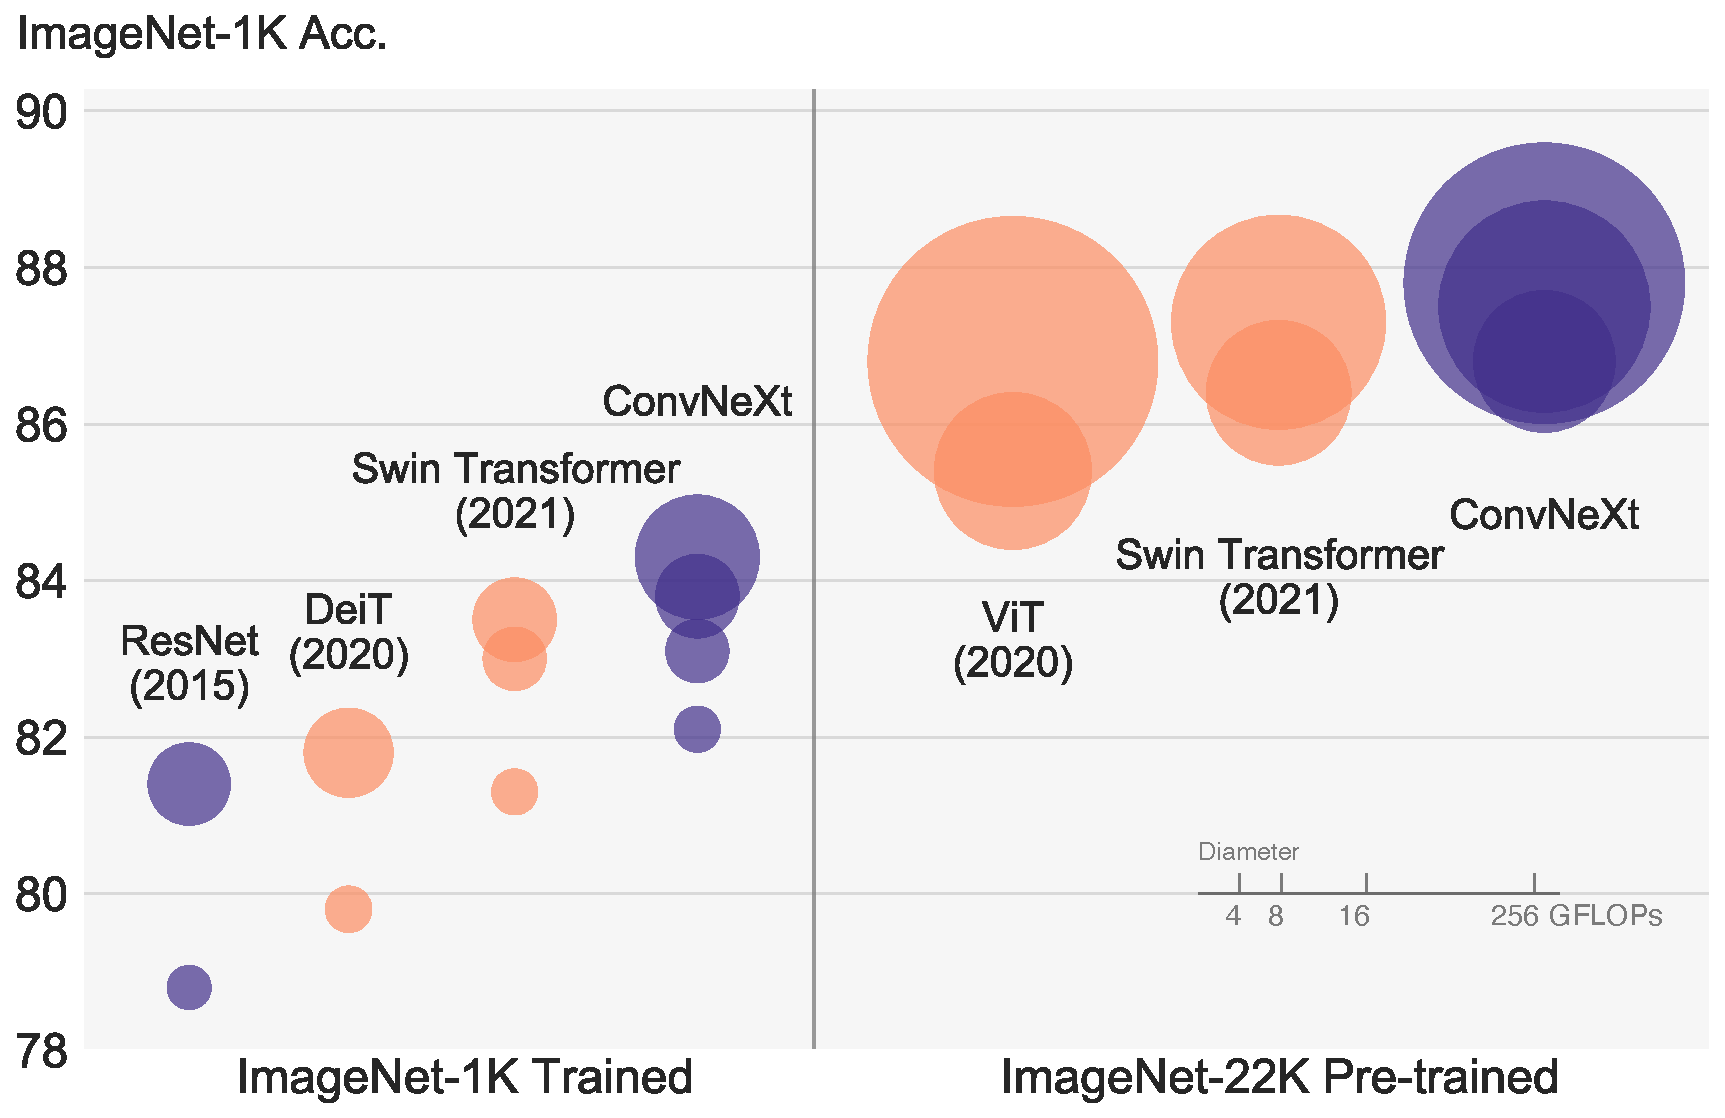
\includegraphics[width=0.8\textwidth]{teaser.pdf}
\caption{\textbf{ImageNet-1K classification} results for \cb ConvNets and \vb vision Transformers. Each bubble's area is proportional to FLOPs of a variant in a model family. ImageNet-1K/22K models here take 224$^2$/384$^2$ images respectively. ResNet and ViT results were obtained with improved training procedures over the original papers. We demonstrate that a standard ConvNet model can achieve the same level of scalability as hierarchical vision Transformers while being much simpler in design.}
\label{fig:teaser}
\end{figure}

The full dominance of ConvNets in computer vision was not a coincidence: in many application scenarios, a ``sliding window'' strategy is intrinsic to visual processing, particularly when working with high-resolution images. ConvNets have several built-in inductive biases that make them well-suited to a wide variety of computer vision applications. The most important one is translation equivariance, which is a desirable property for tasks like objection detection. ConvNets are also inherently efficient due to the fact that when used in a sliding-window manner, the computations are shared~\cite{Sermanet2014}. For many decades, this has been the default use of ConvNets, generally on limited object categories such as digits \cite{lecun1998gradient}, faces \cite{vaillant1994original,rowley1998neural} and pedestrians \cite{sermanet2013pedestrian, dollar2010fastest}. Entering the 2010s, the region-based detectors \cite{rcnn, Girshick2015, Ren2015, He2017} further elevated ConvNets to the position of being the fundamental building block in a visual recognition system. 

Around the same time, the odyssey of neural network design for natural language processing (NLP) took a very different path, as the Transformers replaced recurrent neural networks to become the dominant backbone architecture. Despite the disparity in the task of interest between language and vision domains, the two streams surprisingly converged in the year 2020, as the introduction of Vision Transformers (ViT) completely altered the landscape of network architecture design. Except for the initial ``patchify'' layer, which splits an image into a sequence of patches, ViT introduces no image-specific inductive bias and makes minimal changes to the original NLP Transformers. One primary focus of ViT is on the scaling behavior: with the help of larger model and dataset sizes, Transformers can outperform standard ResNets by a significant margin. Those results on image classification tasks are inspiring, but computer vision is not limited to image classification. As discussed previously, solutions to numerous computer vision tasks in the past decade depended significantly on a sliding-window, fully-convolutional paradigm. Without the ConvNet inductive biases, a vanilla ViT model faces many challenges in being adopted as a generic vision backbone. The biggest challenge is ViT's global attention design, which has a quadratic complexity with respect to the input size. This might be acceptable for ImageNet classification, but quickly becomes intractable with higher-resolution inputs. 

Hierarchical Transformers employ a hybrid approach to bridge this gap. For example, the ``sliding window'' strategy (\eg attention within local windows) was reintroduced to Transformers, allowing them to behave more similarly to ConvNets. Swin Transformer~\cite{Liu2021swin} is a milestone work in this direction, demonstrating for the first time that Transformers can be adopted as a generic vision backbone and achieve state-of-the-art performance across a range of computer vision tasks beyond image classification. Swin Transformer's success and rapid adoption also revealed one thing: the essence of convolution is not becoming irrelevant; rather, it remains much desired and has never faded. 


Under this perspective, many of the advancements of Transformers for computer vision have been aimed at bringing back convolutions. These attempts, however, come at a cost: a naive implementation of sliding window self-attention can be expensive~\cite{ramachandran2019stand}; with advanced approaches such as cyclic shifting~\cite{Liu2021swin}, the speed can be optimized but the system becomes more sophisticated in design. 
On the other hand, it is almost ironic that a ConvNet already satisfies many of those desired properties, albeit in a straightforward, no-frills way. The only reason ConvNets appear to be losing steam is that (hierarchical) Transformers surpass them in many vision tasks, and the performance difference is usually attributed to the superior scaling behavior of Transformers, with multi-head self-attention being the key component. 

Unlike ConvNets, which have progressively improved over the last decade, the adoption of Vision Transformers was a step change. In recent literature, system-level comparisons (\eg a Swin Transformer \vs a ResNet) are usually adopted when comparing the two. ConvNets and hierarchical vision Transformers become different and similar at the same time: they are both equipped with similar inductive biases, but differ significantly in the training procedure and macro/micro-level architecture design. 
In this work, 
we investigate the architectural distinctions between ConvNets and Transformers and try to identify the confounding variables when comparing the network performance.
Our research is intended to bridge the gap between the pre-ViT and post-ViT eras for ConvNets, as well as to test the limits of what a pure ConvNet can achieve. 

To do this, we start with a standard ResNet (\eg ResNet-50) trained with an improved procedure. We gradually ``modernize'' the architecture to the construction of a hierarchical vision Transformer (\eg Swin-T). Our exploration is directed by a key question: \emph{How do design decisions in Transformers impact ConvNets' performance?} We discover several key components that contribute to the performance difference along the way. As a result, we propose a family of \textit{pure ConvNets} dubbed \cnn{}. 
We evaluate \cnn{s} on a variety of vision tasks such as ImageNet classification~\cite{Deng2009}, object detection/segmentation on COCO\cite{Lin2014}, and semantic segmentation on ADE20K~\cite{Zhou2019}. Surprisingly, \cnn{s}, constructed entirely from standard ConvNet modules, compete favorably with Transformers in terms of accuracy, scalability and robustness across all major benchmarks. 
ConvNeXt maintains the efficiency of standard ConvNets, and the fully-convolutional nature for both training and testing makes it extremely simple to implement.

We hope the new observations and discussions can challenge some common beliefs and encourage people to rethink the importance of convolutions in computer vision.

%##################################################################################################
\begin{figure}[!htbp] 
\centering
\includegraphics[width=0.66\textwidth]{morph_main_v3}
\caption{We modernize a standard ConvNet (ResNet) towards the design of a hierarchical vision Transformer (Swin), without introducing any attention-based modules. The foreground bars are model accuracies in the ResNet-50/Swin-T FLOP regime; results for the ResNet-200/Swin-B regime are shown with the gray bars. A hatched bar means the modification is not adopted. Detailed results for both regimes are in the appendix. Many Transformer architectural choices can be incorporated in a ConvNet, and they lead to increasingly better performance. In the end, our pure ConvNet model, named ConvNeXt, can outperform the Swin Transformer.}
\label{fig:morph_main}
\end{figure}
%##################################################################################################

\section{Modernizing a ConvNet: a Roadmap}
\label{sec:modernizing}
In this section, we provide a trajectory going from a ResNet to a ConvNet that bears a resemblance to Transformers. We consider two model sizes in terms of FLOPs, one is the ResNet-50 / Swin-T regime with FLOPs around $4.5\times 10^9$ and the other being ResNet-200 / Swin-B regime which has FLOPs around $15.0\times 10^9$. For simplicity, we will present the results with the ResNet-50 / Swin-T complexity models. The conclusions for higher capacity models are consistent and results can be found in Appendix~\ref{sec:modernizing_result}.

At a high level, our explorations are directed to investigate and follow different levels of designs from a Swin Transformer while maintaining the network's simplicity as a standard ConvNet. The roadmap of our exploration is as follows. Our starting point is a ResNet-50 model. We first train it with similar training techniques used to train vision Transformers and obtain much improved results compared to the original ResNet-50. This will be our baseline. We then study a series of design decisions which we summarized as 1) macro design, 2) ResNeXt, 3) inverted bottleneck, 4) large kernel size, and 5) various layer-wise micro designs. In Figure~\ref{fig:morph_main}, we show the procedure and the results we are able to achieve with each step of the ``network modernization''. Since network complexity is closely correlated with the final performance, the FLOPs are roughly controlled over the course of the exploration, though at intermediate steps the FLOPs might be higher or lower than the reference models. All models are trained and evaluated on ImageNet-1K.


\subsection{Training Techniques}
Apart from the design of the network architecture, the training procedure also affects the ultimate performance. 
Not only did vision Transformers bring a new set of modules and architectural design decisions, but they also introduced different training techniques (\eg AdamW optimizer) to vision.
This pertains mostly to the optimization strategy and associated hyper-parameter settings.
Thus, the first step of our exploration is to train a baseline model with the vision Transformer training procedure, in this case, ResNet-50/200. 
Recent studies~\cite{bello2021revisiting, Wightman2021resnet} demonstrate that a set of modern training techniques can significantly enhance the performance of a simple ResNet-50 model. In our study, we use a training recipe that is close to DeiT's~\cite{Touvron2020} and Swin Transformer's~\cite{Liu2021swin}. The training is extended to 300 epochs from the original 90 epochs for ResNets. We use the AdamW optimizer~\cite{Loshchilov2019}, data augmentation techniques such as Mixup~\cite{Zhang2018a}, Cutmix~\cite{Yun2019}, RandAugment~\cite{Cubuk2020}, Random Erasing~\cite{Zhong2020}, and regularization schemes including Stochastic Depth~\cite{Huang2017} and Label Smoothing~\cite{Szegedy2016a}. The complete set of hyper-parameters we use can be found in Appendix~\ref{subsec:setting}. By itself, this enhanced training recipe increased the performance of the ResNet-50 model from 76.1\% \cite{torchvision} to 78.8\% (+2.7\%), implying that a significant portion of the performance difference between traditional ConvNets and vision Transformers may be due to the training techniques. We will use this fixed training recipe with the same hyperparameters throughout the ``modernization'' process. Each reported accuracy on the ResNet-50 regime is an average obtained from training with three different random seeds.

\subsection{Macro Design}
We now analyze Swin Transformers' macro network design. Swin Transformers follow ConvNets~\cite{vgg, resnet} to use a multi-stage design, where each stage has a different feature map resolution. There are two interesting design considerations: the stage compute ratio, and the ``stem cell'' structure.
\paragraph{Changing stage compute ratio.} 
The original design of the computation distribution across stages in ResNet was largely empirical. The heavy ``res4'' stage was meant to be compatible with downstream tasks like object detection, where a detector head operates on the 14$\times$14 feature plane. 
Swin-T, on the other hand, followed the same principle but with a slightly different stage compute ratio of 1:1:3:1. For larger Swin Transformers, the ratio is 1:1:9:1. Following the design, we adjust the number of blocks in each stage from (3, 4, 6, 3) in ResNet-50 to (3, 3, 9, 3), which also aligns the FLOPs with Swin-T. This improves the model accuracy from 78.8\% to 79.4\%. Notably, researchers have thoroughly investigated the distribution of computation~\cite{Radosavovic2019network, Radosavovic2020designing}, and a more optimal design is likely to exist. 

\textit{From now on, we will use this stage compute ratio.} 

\paragraph{Changing stem to ``Patchify''.}
Typically, the stem cell design is concerned with how the input images will be processed at the network's beginning. Due to the redundancy inherent in natural images, a common stem cell will aggressively downsample the input images to an appropriate feature map size in both standard ConvNets and vision Transformers. The stem cell in standard ResNet contains a 7$\times$7 convolution layer with stride 2, followed by a max pool, which results in a 4$\times$ downsampling of the input images. In vision Transformers, a more aggressive ``patchify'' strategy is used as the stem cell, which corresponds to a large kernel size (e.g. kernel size = 14 or 16) and non-overlapping convolution. Swin Transformer uses a similar ``patchify'' layer, but with a smaller patch size of 4 to accommodate the architecture's multi-stage design. 
We replace the ResNet-style stem cell with a patchify layer implemented using a 4$\times$4, stride 4 convolutional layer. The accuracy has changed from 79.4\% to 79.5\%. This suggests that the stem cell in a ResNet may be substituted with a simpler ``patchify'' layer à la ViT which will result in similar performance.

\textit{We will use the ``patchify stem'' (4$\times$4 non-overlapping convolution) in the network.} 

\subsection{ResNeXt-ify}
In this part, we attempt to adopt the idea of ResNeXt~\cite{Xie2017}, which has a better FLOPs/accuracy trade-off than a vanilla ResNet. The core component is grouped convolution, where the convolutional filters are separated into different groups. At a high level, ResNeXt's guiding principle is to ``use more groups, expand width''. More precisely, ResNeXt employs grouped convolution for the 3$\times$3 conv layer in a bottleneck block. As this significantly reduces the FLOPs, the network width is expanded to compensate for the capacity loss. 

In our case we use depthwise convolution, a special case of grouped convolution where the number of groups equals the number of channels. Depthwise conv has been popularized by MobileNet~\cite{Howard2017} and Xception~\cite{Chollet2017}. We note that depthwise convolution is similar to the weighted sum operation in self-attention, which operates on a per-channel basis, \ie, only mixing information in the spatial dimension. The combination of depthwise conv and $1\times1$ convs leads to a separation of spatial and channel mixing, a property shared by vision Transformers, where each operation either mixes information across spatial or channel dimension, but not both. The use of depthwise convolution effectively reduces the network FLOPs and, as expected, the accuracy. Following the strategy proposed in ResNeXt, we increase the network width to the same number of channels as Swin-T's (from 64 to 96). This brings the network performance to 80.5\% with increased FLOPs (5.3G).
  
\textit{We will now employ the ResNeXt design.}

\subsection{Inverted Bottleneck}
One important design in every Transformer block is that it creates an inverted bottleneck, \ie, the hidden dimension of the MLP block is four times wider than the input dimension (see Figure~\ref{fig:block}). Interestingly, this Transformer design is connected to the inverted bottleneck design with an expansion ratio of 4 used in ConvNets. The idea was popularized by MobileNetV2~\cite{Sandler2018}, and has subsequently gained traction in several advanced ConvNet architectures~\cite{Tan2019efficientnet,tan2019mnasnet}.

Here we explore the inverted bottleneck design. Figure~\ref{fig:inverted} (a) to (b) illustrate the configurations. Despite the increased FLOPs for the depthwise convolution layer, this change reduces the whole network FLOPs to 4.6G, due to the significant FLOPs reduction in the downsampling residual blocks' shortcut 1$\times$1 conv layer.
Interestingly, this results in slightly improved performance (80.5\% to 80.6\%). In the ResNet-200 / Swin-B regime, this step brings even more gain (81.9\% to 82.6\%) also with reduced FLOPs.

\textit{We will now use inverted bottlenecks.}

\subsection{Large Kernel Sizes}

In this part of the exploration, we focus on the behavior of large convolutional kernels. One of the most distinguishing aspects of vision Transformers is their non-local self-attention, which enables each layer to have a global receptive field. While large kernel sizes have been used in the past with ConvNets~\cite{alexnet,Szegedy2015}, the gold standard (popularized by VGGNet~\cite{vgg}) is to stack small kernel-sized (3$\times$3) conv layers, which have efficient hardware implementations on modern GPUs~\cite{Lavin2016FastAF}. Although Swin Transformers reintroduced the local window to the self-attention block, the window size is at least 7$\times$7, significantly larger than the ResNe(X)t kernel size of 3$\times$3. Here we revisit the use of large kernel-sized convolutions for ConvNets. 

\paragraph{Moving up depthwise conv layer.}

\begin{figure}
\centering
\includegraphics[width=0.8\textwidth]{inverted_v2.pdf}
\caption{\textbf{Block modifications and resulted specifications.} \textbf{(a)} is a ResNeXt block; in \textbf{(b)} we create an inverted bottleneck block and in \textbf{(c)} the position of the spatial depthwise conv layer is moved up.}
\label{fig:inverted}
\end{figure}

 To explore large kernels, one prerequisite is to move up the position of the depthwise conv layer (Figure \ref{fig:inverted} (b) to (c)). That is a design decision also evident in Transformers: the MSA block is placed prior to the MLP layers. As we have an inverted bottleneck block, this is a natural design choice --- the complex/inefficient modules (MSA, large-kernel conv) will have fewer channels, while the efficient, dense 1$\times$1 layers will do the heavy lifting. This intermediate step reduces the FLOPs to 4.1G, resulting in a temporary performance degradation to 79.9\%.

\paragraph{Increasing the kernel size.}
With all of these preparations, the benefit of adopting larger kernel-sized convolutions is significant. We experimented with several kernel sizes, including 3, 5, 7, 9, and 11. The network's performance increases from 79.9\% (3$\times$3) to 80.6\% (7$\times$7), while the network's FLOPs stay roughly the same. Additionally, we observe that the benefit of larger kernel sizes reaches a saturation point at 7$\times$7. We verified this behavior in the large capacity model too: a ResNet-200 regime model does not exhibit further gain when we increase the kernel size beyond 7$\times$7. 

\textit{We will use 7$\times$7 depthwise conv in each block.} 

At this point, we have concluded our examination of network architectures on a macro scale. Intriguingly, a significant portion of the design choices taken in a vision Transformer may be mapped to ConvNet instantiations. 

\subsection{Micro Design}
In this section, we investigate several other architectural differences at a micro scale --- most of the explorations here are done at the layer level, focusing on specific choices of activation functions and normalization layers.  
\paragraph{Replacing ReLU with GELU}
One discrepancy between NLP and vision architectures is the specifics of which activation functions to use. Numerous activation functions have been developed over time, but the Rectified Linear Unit (ReLU)~\cite{Nair2010} is still extensively used in ConvNets due to its simplicity and efficiency. ReLU is also used as an activation function in the original Transformer paper~\cite{Vaswani2017}. The Gaussian Error Linear Unit, or GELU~\cite{Hendrycks2016}, which can be thought of as a smoother variant of ReLU, is utilized in the most advanced Transformers, including Google's BERT~\cite{Devlin2019} and OpenAI's GPT-2~\cite{Radford2019}, and, most recently, ViTs. We find that ReLU can be substituted with GELU in our ConvNet too, although the accuracy stays unchanged (80.6\%).
 

\paragraph{Fewer activation functions.}
One minor distinction between a Transformer and a ResNet block is that Transformers have fewer activation functions. Consider a Transformer block with key/query/value linear embedding layers, the projection layer, and two linear layers in an MLP block. There is only one activation function present in the MLP block. In comparison, it is common practice to append an activation function to each convolutional layer, including the $1\times1$ convs. Here we examine how performance changes when we stick to the same strategy. As depicted in Figure~\ref{fig:block}, we eliminate all GELU layers from the residual block except for one between two $1\times1$ layers, replicating the style of a Transformer block. This process improves the result by 0.7\% to 81.3\%, practically matching the performance of Swin-T. 


\textit{We will now use a single GELU activation in each block.}

\begin{figure}[t]
\centering
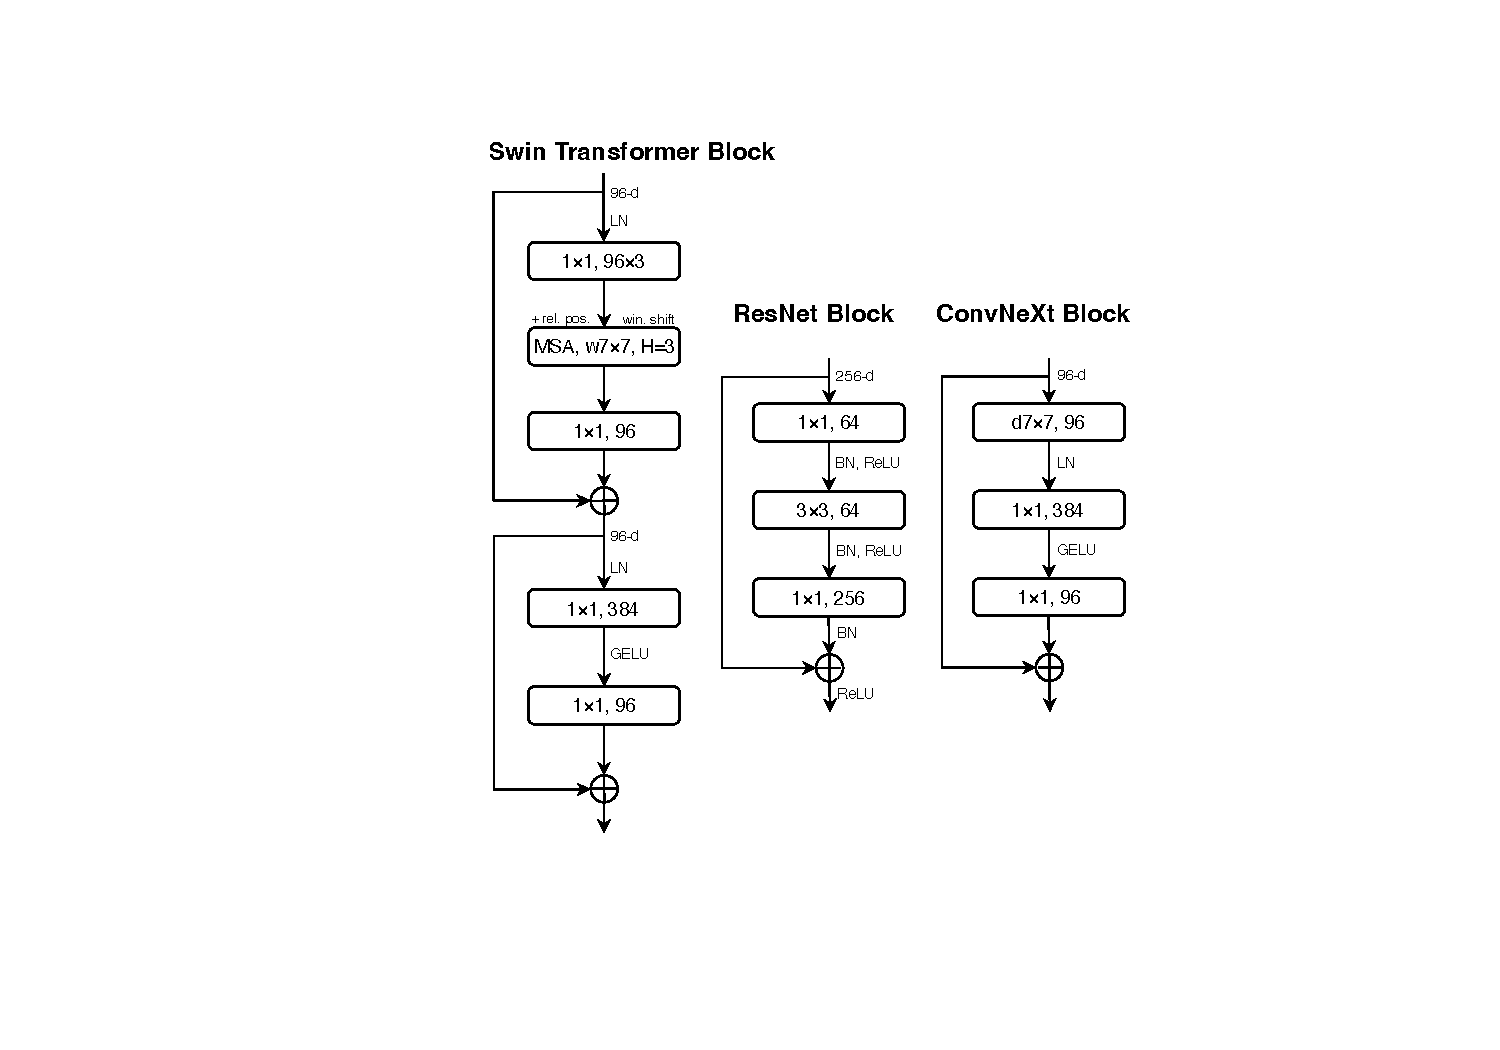
\includegraphics[width=0.75\textwidth]{block_v4.pdf}
\caption{\textbf{Block designs} for a ResNet, a Swin Transformer, and a \cnn. Swin Transformer's block is more sophisticated due to the presence of multiple specialized modules and two residual connections. For simplicity, we note the linear layers in Transformer MLP blocks also as ``1$\times$1 convs'' since they are equivalent.}
\label{fig:block}
\end{figure}

\paragraph{Fewer normalization layers.}
Transformer blocks usually have fewer normalization layers as well. Here we remove two BatchNorm (BN) layers, leaving only one BN layer before the conv $1\times1$ layers. This further \textit{boosts} the performance to 81.4\%, already surpassing Swin-T's result. Note that we have even fewer normalization layers per block than Transformers, as empirically we find that adding one additional BN layer at the beginning of the block does not improve the performance. 

\paragraph{Substituting BN with LN.}
BatchNorm~\cite{Ioffe2017} is an essential component in ConvNets as it improves the convergence and reduces overfitting. However, BN also has many intricacies that can have a detrimental effect on the model's performance~\cite{wu2021rethinking}. There have been numerous attempts at developing alternative normalization~\cite{Salimans2016,Ulyanov2016,Wu2018} techniques, but BN has remained the preferred option in most vision tasks.
On the other hand, the simpler Layer Normalization~\cite{Ba2016} (LN) has been used in Transformers, resulting in good performance across different application scenarios.

Directly substituting LN for BN in the original ResNet will result in suboptimal performance~\cite{Wu2018}. With all the modifications in network architecture and training techniques, here we revisit the impact of using LN in place of BN. We observe that our ConvNet model does not have any difficulties training with LN; in fact, the performance is slightly better, obtaining an accuracy of 81.5\%.


\textit{From now on, we will use one LayerNorm as our choice of normalization in each residual block.}
 
\paragraph{Separate downsampling layers.}

In ResNet, the spatial downsampling is achieved by the residual block at the start of each stage, using 3$\times$3 conv with stride 2 (and 1$\times$1 conv with stride 2 at the shortcut connection). In Swin Transformers, a separate downsampling layer is added between stages. We explore a similar strategy in which we use 2$\times$2 conv layers with stride 2 for spatial downsampling. This modification surprisingly leads to diverged training. Further investigation shows that, adding normalization layers wherever spatial resolution is changed can help stablize training. These include several LN layers also used in Swin Transformers: one before each downsampling layer, one after the stem, and one after the final global average pooling. 
We can improve the accuracy to 82.0\%, significantly exceeding Swin-T's 81.3\%.


\textit{
We will use separate downsampling layers. This brings us to our final model, which we have dubbed \cnn{}.}

\textit{A comparison of ResNet, Swin, and \cnn{} block structures can be found in Figure \ref{fig:block}. A comparison of ResNet-50, Swin-T and \cnn{}-T's detailed architecture specifications can be found in Table~\ref{table:arch-spec}.}

\paragraph{Closing remarks.}
We have finished our first ``playthrough'' and discovered \cnn{}, a pure ConvNet, that can outperform the Swin Transformer for ImageNet-1K classification in this compute regime. 
It is worth noting that \emph{all design choices discussed so far are adapted from vision Transformers. \emph{In addition,} these designs are not novel even in the ConvNet literature --- they have all been researched separately, but not collectively, over the last decade.}
Our \cnn{} model has approximately the same FLOPs, \#params., throughput, and memory use as the Swin Transformer, but does not require specialized modules such as shifted window attention or relative position biases. 

These findings are encouraging but not yet completely convincing --- our exploration thus far has been limited to a small scale, but vision Transformers' scaling behavior is what truly distinguishes them. Additionally, the question of whether a ConvNet can compete with Swin Transformers on downstream tasks such as object detection and semantic segmentation is a central concern for computer vision practitioners.
In the next section, we will scale up our \cnn{} models both in terms of data and model size, and evaluate them on a diverse set of visual recognition tasks.


\section{Experiments on ImageNet}
\label{sec:convnext_config}
 We construct different \cnn{} variants, \cnn{}-T/S/B/L, to be of similar complexities to Swin-T/S/B/L \cite{Liu2021swin}. \cnn{}-T/B is the end product of the ``modernizing'' procedure on ResNet-50/200 regime, respectively. In addition, we build a larger \cnn{}-XL to further test the scalability of \cnn{}. The variants only differ in the number of channels $C$, and the number of blocks $B$ in each stage. Following both ResNets and Swin Transformers, the number of channels doubles at each new stage. We summarize the configurations below:
\begin{itemize}[leftmargin=-.1ex]
\setlength\itemsep{-.2em}
% \small{
\item[]\cb\cnn{-T}: $C=(96,192,384,768)$, $B=(3,3,9,3)$
\item[]\cb\cnn{-S}: $C=(96,192,384,768)$, $B=(3,3,27,3)$
\item[]\cb\cnn{-B}: $C=(128,256,512,1024)$, $B=(3,3,27,3)$
\item[]\cb\cnn{-L}: $C=(192,384,768,1536)$, $B=(3,3,27,3)$
\item[]\cb\cnn{-XL}: $C=(256,512,1024,2048)$, $B=(3,3,27,3)$
% }
\end{itemize}


\subsection{Settings}
The ImageNet-1K dataset consists of 1000 object classes with 1.2M training images. We report ImageNet-1K top-1 accuracy on the validation set. We also conduct pre-training on ImageNet-22K, a larger dataset of 21841 classes (a superset of the 1000 ImageNet-1K classes) with $\sim$14M images for pre-training, and then fine-tune the pre-trained model on ImageNet-1K for evaluation.  We summarize our training setups below. More details can be found in Appendix~\ref{sec:setting}. 

\paragraph{Training on ImageNet-1K.} We train \cnn{}s for 300 epochs using AdamW~\cite{Loshchilov2019} with a learning rate of 4e-3. There is a 20-epoch linear warmup and a cosine decaying schedule afterward. We use a batch size of 4096 and a weight decay of 0.05. For data augmentations, we adopt common schemes including Mixup~\cite{Zhang2018a}, Cutmix~\cite{Yun2019}, RandAugment~\cite{Cubuk2020}, and Random Erasing~\cite{Zhong2020}. We regularize the networks with Stochastic Depth~\cite{Huang2016deep} and Label Smoothing~\cite{Szegedy2016a}. Layer Scale~\cite{Touvron2021GoingDW} of initial value 1e-6 is applied. We use Exponential Moving Average (EMA)~\cite{Polyak1992} as we find it alleviates larger models' overfitting.

\paragraph{Pre-training on ImageNet-22K.} We pre-train \cnn{}s on ImageNet-22K for 90 epochs with a warmup of 5 epochs. We do not use EMA. Other settings follow ImageNet-1K.

\paragraph{Fine-tuning on ImageNet-1K.}
We fine-tune ImageNet-22K pre-trained models on ImageNet-1K for 30 epochs. We use AdamW, a learning rate of 5e-5, cosine learning rate schedule, layer-wise learning rate decay~\cite{Clark2020,Bao2021}, no warmup, a batch size of 512, and weight decay of 1e-8. 
The default pre-training, fine-tuning, and testing resolution is 224$^2$. Additionally, we fine-tune at a larger resolution of 384$^2$, for both ImageNet-22K and ImageNet-1K pre-trained models. 

Compared with ViTs/Swin Transformers, \cnn{}s are simpler to fine-tune at different resolutions, as the network is fully-convolutional and there is no need to adjust the input patch size or interpolate absolute/relative position biases.

%##################################################################################################
\begin{table}[!htbp]
\centering
% \small
\footnotesize
\addtolength{\tabcolsep}{-5.pt}
\begin{tabular}{lccccc}
   model & \begin{tabular}[c]{@{}c@{}}image \\ size\end{tabular} & \#param. & FLOPs & \begin{tabular}[c]{@{}c@{}}throughput\\ (image / s)\end{tabular} & \begin{tabular}[c]{@{}c@{}} IN-1K \\ top-1 acc.\end{tabular} \\
\Xhline{1.0pt}
\multicolumn{6}{c}{\scriptsize{ImageNet-1K trained models}} \\
\cb RegNetY-16G~\cite{Radosavovic2020designing} & 224$^2$ & 84M & 16.0G & 334.7 & 82.9 \\
\cb EffNet-B7~\cite{Tan2019efficientnet} & 600$^2$ & 66M & 37.0G & 55.1 & 84.3 \\
\cb EffNetV2-L~\cite{tan2021efficientnetv2} & 480$^2$ & 120M & 53.0G & 83.7 & 85.7 \\

\hline

\vb DeiT-S~\cite{Touvron2020} & 224$^2$ & 22M & 4.6G & 978.5 & 79.8 \\ 
\vb DeiT-B~\cite{Touvron2020} & 224$^2$ & 87M & 17.6G & 302.1 & 81.8 \\
\hline
\vb Swin-T   & 224$^2$ & 28M & 4.5G & 757.9 & 81.3 \\
\gr
\cb \cnn{}-T & 224$^2$ & 29M & 4.5G & 774.7 & \textbf{82.1} \\ 

\vb Swin-S   & 224$^2$ & 50M & 8.7G & 436.7 & 83.0 \\
\gr
\cb \cnn{}-S & 224$^2$ & 50M & 8.7G & 447.1 & \textbf{83.1} \\ 

\vb Swin-B   & 224$^2$ & 88M & 15.4G& 286.6& 83.5 \\
\gr
\cb \cnn{}-B & 224$^2$ & 89M & 15.4G& 292.1& \textbf{83.8} \\ 

\vb Swin-B   & 384$^2$ & 88M & 47.1G& 85.1 & 84.5 \\
\gr
\cb \cnn{}-B & 384$^2$ & 89M & 45.0G& 95.7 & \textbf{85.1} \\

\gr
\cb \cnn{}-L & 224$^2$ & 198M & 34.4G & 146.8 & \textbf{84.3} \\
\gr
\cb \cnn{}-L & 384$^2$ & 198M & 101.0G& 50.4 & \textbf{85.5} \\
\hline


\multicolumn{6}{c}{\scriptsize{ImageNet-22K pre-trained models}}  \\  
\cb R-101x3~\cite{Kolesnikov2020} & 384$^2$ & 388M & 204.6G & - & 84.4 \\
\cb R-152x4~\cite{Kolesnikov2020} & 480$^2$ & 937M & 840.5G & - & 85.4 \\
\cb EffNetV2-L~\cite{tan2021efficientnetv2} & 480$^2$ & 120M & 53.0G & 83.7 & 86.8 \\
\cb EffNetV2-XL~\cite{tan2021efficientnetv2} & 480$^2$ & 208M & 94.0G & 56.5 & 87.3 \\

\hline
\vb ViT-B/16 (\Telefon)~\cite{steiner2021train} & 384$^2$ & 87M & 55.5G & 93.1 & 85.4 \\ 
\vb ViT-L/16 (\Telefon)~\cite{steiner2021train} & 384$^2$ & 305M & 191.1G & 28.5 & 86.8 \\

\hline

\gr
\cb \cnn{}-T & 224$^2$ & 29M  & 4.5G & 774.7 & \textbf{82.9} \\
\gr
\cb \cnn{}-T & 384$^2$ & 29M  & 13.1G & 282.8 & \textbf{84.1} \\
\gr
\cb \cnn{}-S & 224$^2$ & 50M  & 8.7G & 447.1 & \textbf{84.6} \\
\gr
\cb \cnn{}-S & 384$^2$ & 50M  & 25.5G & 163.5 & \textbf{85.8} \\

\vb Swin-B   & 224$^2$ & 88M  & 15.4G & 286.6 & 85.2          \\
\gr
\cb \cnn{}-B & 224$^2$ & 89M  & 15.4G & 292.1 & \textbf{85.8} \\

\vb Swin-B   & 384$^2$ & 88M  & 47.0G & 85.1  & 86.4          \\
\gr
\cb \cnn{}-B & 384$^2$ & 89M  & 45.1G & 95.7  & \textbf{86.8} \\

\vb Swin-L   & 224$^2$ & 197M & 34.5G & 145.0 &  86.3         \\
\gr
\cb \cnn{}-L & 224$^2$ & 198M & 34.4G & 146.8 & \textbf{86.6}\\

\vb Swin-L   & 384$^2$ & 197M & 103.9G& 46.0  & 87.3          \\
\gr
\cb \cnn{}-L & 384$^2$ & 198M & 101.0G& 50.4  & \textbf{87.5}  \\
\gr
\cb \cnn{}-XL & 224$^2$ & 350M & 60.9G & 89.3  & \textbf{87.0}  \\
\gr
\cb \cnn{}-XL & 384$^2$ & 350M & 179.0G& 30.2  & \textbf{87.8}  \\

\hline
\end{tabular}
\normalsize
\caption{\textbf{Classification accuracy on ImageNet-1K.} Similar to Transformers, \cnn{} also shows promising scaling behavior with higher-capacity models and a larger (pre-training) dataset. Inference throughput is measured on a V100 GPU, following~\cite{Liu2021swin}. On an A100 GPU, \cnn{} can have a much higher throughput than Swin Transformer. See Appendix~\ref{sec:a100}. (\Telefon)ViT results with 90-epoch AugReg~\cite{steiner2021train} training, provided through personal communication with the authors.}
\label{tab:imagenet-system}
\end{table}

\subsection{Results}
\label{subsec:imagenet-results}
\paragraph{ImageNet-1K.} Table \ref{tab:imagenet-system} (upper) shows the result comparison with two recent Transformer variants, DeiT \cite{Touvron2020} and Swin Transformers \cite{Liu2021swin}, as well as two ConvNets from architecture search - RegNets~\cite{Radosavovic2020designing}, EfficientNets~\cite{Tan2019efficientnet} and EfficientNetsV2~\cite{tan2021efficientnetv2}. \cnn{} competes favorably with two strong ConvNet baselines (RegNet~\cite{Radosavovic2020designing} and EfficientNet~\cite{Tan2019efficientnet}) in terms of the accuracy-computation trade-off, as well as the inference throughputs. \cnn{} also outperforms Swin Transformer of similar complexities \emph{across the board}, sometimes with a substantial margin (\eg 0.8\% for \cnn{}-T). Without specialized modules such as shifted windows or relative position bias, \cnn{s} also enjoy improved throughput compared to Swin Transformers.

A highlight from the results is \cnn{}-B at 384$^2$: it outperforms Swin-B by 0.6\% (85.1\% vs. 84.5\%), but with 12.5\% higher inference throughput (95.7 vs. 85.1 image/s). We note that the FLOPs/throughput advantage of \cnn{}-B over Swin-B becomes larger when the resolution increases from 224$^2$ to 384$^2$. Additionally, we observe an improved result of 85.5\% when further scaling to \cnn{}-L.

\paragraph{ImageNet-22K.}
We present results with models fine-tuned from ImageNet-22K pre-training at Table \ref{tab:imagenet-system} (lower). 
These experiments are important since a widely held view is that vision Transformers have fewer inductive biases thus can perform better than ConvNets when pre-trained on a larger scale. 
 Our results demonstrate that properly designed ConvNets are \emph{not} inferior to vision Transformers when pre-trained with large dataset --- \cnn{s} still perform on par or better than similarly-sized Swin Transformers, with slightly higher throughput. Additionally, our \cnn{}-XL model achieves an accuracy of 87.8\% --- a decent improvement over \cnn{}-L at 384$^2$, demonstrating that \cnn{}s are scalable architectures. 
 
On ImageNet-1K, EfficientNetV2-L, a searched architecture equipped with advanced modules (such as Squeeze-and-Excitation~\cite{hu2018squeeze}) and progressive training procedure achieves top performance. However, with ImageNet-22K pre-training, ConvNeXt is able to outperform EfficientNetV2, further demonstrating the importance of large-scale training.

In Appendix~\ref{sec:robustness}, we discuss robustness and out-of-domain generalization results for \cnn{}.

\subsection{Isotropic \cnn{} \vs ViT}
\label{subsec:isotropic} 
In this ablation, we examine if our \cnn{} block design is generalizable to ViT-style~\cite{Dosovitskiy2021} isotropic architectures which have no downsampling layers and keep the same feature resolutions (\eg 14$\times$14) at all depths. We construct isotropic \cnn{}-S/B/L using the same feature dimensions as ViT-S/B/L (384/768/1024). Depths are set at 18/18/36 to match the number of parameters and FLOPs. The block structure remains the same (Fig.~\ref{fig:block}).
We use the supervised training results from DeiT \cite{Touvron2020} for ViT-S/B and MAE~\cite{he2021masked} for ViT-L, as they employ improved training procedures over the original ViTs \cite{Dosovitskiy2021}. \cnn{} models are trained with the same settings as before, but with longer warmup epochs. Results for ImageNet-1K at 224$^2$ resolution are in Table \ref{tab:non-hie}. We observe \cnn{} can perform generally on par with ViT, showing that our \cnn{} block design is competitive when used in non-hierarchical models. 

%##################################################################################################
\begin{table}[!htbp]
\tablestyle{2pt}{1.0}
% \hspace{-1em}
\normalsize
\begin{tabular}{lcccccc}
 model & \#param. & FLOPs & \begin{tabular}[c]{@{}c@{}} throughput\\ (image / s) \end{tabular} & \begin{tabular}[c]{@{}c@{}} training \\ mem. (GB) \end{tabular} &  \begin{tabular}[c]{@{}c@{}}IN-1K \\ acc.\end{tabular} & \\
\shline
\vb ViT-S                         & 22M & 4.6G   &  978.5 & 4.9 & 79.8 \\
\gr
\cb \cnn{}-S (\textit{iso.})      & 22M & 4.3G   &  1038.7& 4.2 & 79.7 \\
\vb ViT-B                         & 87M & 17.6G  &  302.1 & 9.1 & 81.8 \\
\gr
\cb \cnn{}-B (\textit{iso.})      & 87M & 16.9G  &  320.1 & 7.7 & 82.0 \\
\vb ViT-L                         & 304M& 61.6G  &  93.1  & 22.5 & 82.6 \\
\gr
\cb \cnn{}-L (\textit{iso.})      & 306M& 59.7G  &  94.4  & 20.4 & 82.6 \\
\end{tabular}
\caption{\textbf{Comparing isotropic \cnn{} and ViT.} Training memory is measured on V100 GPUs with 32 per-GPU batch size.}
\label{tab:non-hie}
\end{table}
%##################################################################################################

\section{Experiments on Downstream Tasks}
\subsection{Object detection and segmentation on COCO.}

We fine-tune Mask R-CNN~\cite{He2017} and Cascade Mask R-CNN~\cite{Cai2018} on the COCO dataset with \cnn{} backbones. Following Swin Transformer~\cite{Liu2021swin}, we use multi-scale training, AdamW optimizer, and a 3$\times$ schedule. Further details and hyper-parameter settings can be found in Appendix~\ref{subsec:downstream-setting}.


Table~\ref{tab:coco} shows object detection and instance segmentation results comparing Swin Transformer, \cnn{}, and traditional ConvNet such as ResNeXt. Across different model complexities, \cnn{} achieves on-par or better performance than Swin Transformer. When scaled up to bigger models (\cnn{}-B/L/XL) pre-trained on ImageNet-22K, in many cases \emph{ConvNeXt is significantly better} (\eg +1.0 AP) than Swin Transformers in terms of box and mask AP.


\begin{table}[!htbp]
\tablestyle{6pt}{1.1}
% \addtolength{\tabcolsep}{-4.5pt}
\scalebox{1.1}{
\begin{tabular}{@{}lcccccccc@{}}
backbone & FLOPs & FPS & $\text{AP}^{\text{box}}$ & $\text{AP}^{\text{box}}_{50}$ & $\text{AP}^{\text{box}}_{75}$ & $\text{AP}^{\text{mask}}$ & $\text{AP}^{\text{mask}}_{\text{50}}$ & $\text{AP}^{\text{mask}}_{75}$  \\
\shline
\multicolumn{9}{c}{\scriptsize{Mask-RCNN 3$\times$ schedule}} \\
\vb Swin-T      & 267G & 23.1     & 46.0 & 68.1 & 50.3 & 41.6 & 65.1 & 44.9 \\
\gr
\cb \cnn{}-T    & 262G & 25.6     & \textbf{46.2} & 67.9 & 50.8 & \textbf{41.7} & 65.0 & 44.9 \\
\hline
\multicolumn{9}{c}{\scriptsize{Cascade Mask-RCNN 3$\times$ schedule}} \\
\cb ResNet-50            & 739G & 16.2     & 46.3 & 64.3 & 50.5 & 40.1 & 61.7 & 43.4 \\
\cb X101-32              & 819G & 13.8  & 48.1 & 66.5 & 52.4 & 41.6 & 63.9 & 45.2 \\
\cb X101-64              & 972G & 12.6  & 48.3 & 66.4 & 52.3 & 41.7 & 64.0 & 45.1 \\
\Xhline{0.3\arrayrulewidth}
\vb Swin-T               & 745G & 12.2     & 50.4 & 69.2 & 54.7 & 43.7 & 66.6 & 47.3 \\
\gr
\cb \cnn{}-T             & 741G & 13.5     & \textbf{50.4} & 69.1 & 54.8 & \textbf{43.7} & 66.5 & 47.3 \\
\vb Swin-S               & 838G & 11.4     & 51.9	& 70.7	& 56.3	& 45.0	& 68.2	& 48.8 \\
\gr
\cb \cnn{}-S             & 827G & 12.0     & \textbf{51.9} & 70.8 & 56.5 & \textbf{45.0} & 68.4 & 49.1 \\
\vb Swin-B               & 982G & 10.7     & 51.9 & 70.5 & 56.4 & 45.0 & 68.1 & 48.9 \\
\gr
\cb \cnn{}-B             & 964G & 11.4     & \textbf{52.7} & 71.3 & 57.2 & \textbf{45.6} & 68.9 & 49.5 \\
\Xhline{0.3\arrayrulewidth}
\vb Swin-B$^\ddag$               & 982G & 10.7     &  53.0	& 71.8 & 57.5 & 45.8 & 69.4 & 49.7 \\
\gr
\cb \cnn{}-B$^\ddag$             & 964G & 11.5     & \textbf{54.0} & 73.1 & 58.8	& \textbf{46.9}	& 70.6 & 51.3 \\
\vb Swin-L$^\ddag$       & 1382G & 9.2  & 53.9 & 72.4 & 58.8 & 46.7 & 70.1 & 50.8 \\
\gr
\cb \cnn{}-L$^\ddag$     & 1354G & 10.0     & \textbf{54.8} & 73.8 & 59.8 & \textbf{47.6} & 71.3 & 51.7 \\
\gr
\cb \cnn{}-XL$^\ddag$     & 1898G & 8.6     & \textbf{55.2} & 74.2 & 59.9 & \textbf{47.7} & 71.6 & 52.2\\
\end{tabular}
} 
\caption[caption]{\textbf{COCO object detection and segmentation results} using Mask-RCNN and Cascade Mask-RCNN. $^\ddag$ indicates that the model is pre-trained on ImageNet-22K. ImageNet-1K pre-trained Swin results are from their Github repository~\cite{swindetcode}. AP numbers of the ResNet-50 and X101 models are from \cite{Liu2021swin}. We measure FPS on an A100 GPU. FLOPs are calculated with image size (1280, 800).
\label{tab:coco}
}
\end{table}


\subsection{Semantic segmentation on ADE20K.}
We also evaluate \cnn{} backbones on the ADE20K semantic segmentation task with UperNet~\cite{Xiao2018}. All model variants are trained for 160K iterations with a batch size of 16. Other experimental settings follow~\cite{Bao2021} (see Appendix~\ref{subsec:downstream-setting} for more details). In Table \ref{tab:seg}, we report validation mIoU with multi-scale testing. \cnn{} models can achieve competitive performance across different model capacities, further validating the effectiveness of our architecture design. 

\begin{table}[!htbp]
    \centering
    % \small
\addtolength{\tabcolsep}{-2.1pt}
\begin{tabular}{lcccc}
backbone & input crop. & mIoU & \#param. & FLOPs  \\
\Xhline{1.0pt}
\multicolumn{5}{c}{\scriptsize{ImageNet-1K pre-trained}} \\
\vb Swin-T & 512$^2$ & 45.8 & 60M & 945G  \\
\gr
\cb \cnn{}-T &  512$^2$ & \textbf{46.7} & 60M & 939G  \\
\vb Swin-S &  512$^2$ & 49.5 & 81M & 1038G  \\
\gr
\cb \cnn{}-S &  512$^2$ & \textbf{49.6} & 82M & 1027G  \\
\vb Swin-B &  512$^2$ & 49.7 & 121M & 1188G  \\
\gr
\cb \cnn{}-B &  512$^2$ & \textbf{49.9} & 122M & 1170G  \\
\hline
\multicolumn{4}{c}{\scriptsize{ImageNet-22K pre-trained}} \\
\vb Swin-B$^\ddag$ &  640$^2$ & 51.7 & 121M & 1841G  \\
\gr
\cb \cnn{}-B$^\ddag$ & 640$^2$ & \textbf{53.1} & 122M & 1828G  \\
\vb Swin-L$^\ddag$ & 640$^2$ & 53.5 & 234M & 2468G  \\
\gr
\cb \cnn{}-L$^\ddag$ & 640$^2$ & \textbf{53.7} & 235M & 2458G  \\
\gr
\cb \cnn{}-XL$^\ddag$ & 640$^2$ & \textbf{54.0} &  391M & 3335G  \\
\Xhline{1.0pt}
\end{tabular}
    \caption[caption]{\textbf{ADE20K validation results} using UperNet~\cite{Xiao2018}. $^\ddag$ indicates IN-22K  pre-training. Swins' results are from its GitHub repository~\cite{swincode}. Following Swin, we report mIoU results with multi-scale testing. FLOPs are based on input sizes of (2048, 512) and (2560, 640) for IN-1K and IN-22K pre-trained models, respectively.}
    \label{tab:seg}
    \normalsize
\end{table}

\subsection{Remarks on model efficiency.} Under similar FLOPs, models with depthwise convolutions are known to be slower and consume more memory than ConvNets with only dense convolutions. It is natural to ask whether the design of \cnn{} will render it practically inefficient. As demonstrated throughout the paper, the inference throughputs of \cnn{s} are comparable to or exceed that of Swin Transformers. This is true for both classification and other tasks requiring higher-resolution inputs (see Table~\ref{tab:imagenet-system},\ref{tab:coco} for comparisons of throughput/FPS). Furthermore, we notice that training \cnn{s} requires less memory than training Swin Transformers. For example, training Cascade Mask-RCNN using \cnn{}-B backbone consumes 17.4GB of peak memory with a per-GPU batch size of 2, while the reference number for Swin-B is 18.5GB.
In comparison to vanilla ViT, both \cnn{} and Swin Transformer exhibit a more favorable accuracy-FLOPs trade-off due to the local computations. It is worth noting that this improved efficiency is a result of the \emph{ConvNet inductive bias}, and is not directly related to the self-attention mechanism in vision Transformers.


\section{Related Work}
\subsection{Hybrid models} 
In both the pre- and post-ViT eras, the hybrid model combining convolutions and self-attentions has been actively studied. 
Prior to ViT, the focus was on augmenting a ConvNet with self-attention/non-local modules~\cite{Wang2018,bello2019attention,srinivas2021bottleneck,ramachandran2019stand} to capture long-range dependencies.
The original ViT~\cite{Dosovitskiy2021} first studied a hybrid configuration, and a large body of follow-up works focused on reintroducing convolutional priors to ViT, either in an explicit~\cite{wu2021cvt, xu2021co, d2021convit, dai2021coatnet,Xiao2021, fan2021multiscale} or implicit~\cite{Liu2021swin} fashion.

\subsection{Recent convolution-based approaches} 
Han \emph{et al.}~\cite{han2021demystifying} show that local Transformer attention is equivalent to inhomogeneous dynamic depthwise conv. The MSA block in Swin is then replaced with a dynamic or regular depthwise convolution, achieving comparable performance to Swin. A concurrent work ConvMixer~\cite{convmixer} demonstrates that, in small-scale settings, depthwise convolution can be used as a promising mixing strategy. ConvMixer uses a smaller patch size to achieve the best results, making the throughput much lower than other baselines. GFNet~\cite{rao2021global} adopts Fast Fourier Transform (FFT) for token mixing. FFT is also a form of convolution, but with a global kernel size and circular padding. Unlike many recent Transformer or ConvNet designs, one primary goal of our study is to provide an in-depth look at the process of modernizing a standard ResNet and achieving state-of-the-art performance.



% \section*{\Large{Appendix}}
% In this Appendix, we provide further experimental details (\S \ref{sec:setting}), robustness evaluation results (\S \ref{sec:robustness}), more modernization experiment results (\S\ref{sec:modernizing_result}), and a detailed network specification (\S \ref{sec:arch}). We further benchmark model throughput on A100 GPUs (\S \ref{sec:a100}). Finally, we discuss the limitations (\S \ref{sec:limit}) and societal impact (\S \ref{sec:impact}) of our work.

\section{Full Experimental Settings}
\label{sec:setting}
\subsection{ImageNet (Pre-)training} 
\label{subsec:setting}
We provide \cnn{s}' ImageNet-1K training and ImageNet-22K pre-training settings in Table~\ref{tab:train_detail}. The settings are used for our main results in Table~\ref{tab:imagenet-system} (Section~\ref{subsec:imagenet-results}).  All \cnn{} variants use the same setting, except the stochastic depth rate is customized for model variants. 
% For weight initialization, we use a truncated normal distribution with 0.2 standard deviation.

For experiments in ``modernizing a ConvNet'' (Section~\ref{sec:modernizing}), we also use Table~\ref{tab:train_detail}'s setting for ImageNet-1K, except EMA is disabled, as we find using EMA severely hurts models with BatchNorm layers.

For isotropic \cnn{}s (Section~\ref{subsec:isotropic}), the setting for ImageNet-1K in Table~\ref{sec:setting} is also adopted, but warmup is extended to 50 epochs, and layer scale is disabled for isotropic \cnn{}-S/B. The stochastic depth rates are 0.1/0.2/0.5 for isotropic \cnn{}-S/B/L.

\begin{table}[!htbp]
\tablestyle{5.0pt}{1.2}
% \footnotesize
% \large
% \normalsize
\small
\begin{tabular}{@{\hskip -0.05ex}l|c@{\hskip 1ex}c}
& \cnn{}-T/S/B/L & \cnn{}-T/S/B/L/XL \\
\multirow{2}{*}{(pre-)training config} & ImageNet-1K & ImageNet-22K \\
& 224$^2$ & 224$^2$ \\
\shline
weight init & trunc. normal (0.2) & trunc. normal (0.2) \\
optimizer & AdamW & AdamW\\
base learning rate & 4e-3 & 4e-3 \\
weight decay & 0.05 & 0.05 \\
optimizer momentum & $\beta_1, \beta_2{=}0.9, 0.999$ & $\beta_1, \beta_2{=}0.9, 0.999$ \\
batch size & 4096 & 4096 \\
training epochs & 300 & 90 \\
learning rate schedule & cosine decay & cosine decay \\
warmup epochs & 20 & 5 \\
warmup schedule & linear & linear \\
layer-wise lr decay \cite{Clark2020,Bao2021} & None & None \\
randaugment \cite{Cubuk2020} & (9, 0.5) & (9, 0.5) \\
mixup \cite{Zhang2018a} & 0.8 & 0.8 \\
cutmix \cite{Yun2019} & 1.0 & 1.0 \\
random erasing \cite{Zhong2020} & 0.25 & 0.25 \\
label smoothing \cite{Szegedy2016a} & 0.1 & 0.1 \\
stochastic depth \cite{Huang2016deep} & 0.1/0.4/0.5/0.5 & 0.0/0.0/0.1/0.1/0.2 \\
layer scale \cite{Touvron2021GoingDW} & 1e-6 & 1e-6 \\
head init scale \cite{Touvron2021GoingDW} & None & None \\
gradient clip & None & None \\
exp. mov. avg. (EMA) \cite{Polyak1992} & 0.9999 & None\\

\end{tabular}
\caption{\textbf{ImageNet-1K/22K (pre-)training settings}. Multiple stochastic depth rates (e.g., 0.1/0.4/0.5/0.5) are for each model (e.g., \cnn{}-T/S/B/L) respectively.}
\label{tab:train_detail}
\end{table}

\begin{table}[!htbp]
\tablestyle{5.0pt}{1.2}
% \footnotesize
% \normalsize
\small
\begin{tabular}{@{\hskip -0.05ex}l@{\hskip 2.6ex}|cc}
 &  \cnn{-B/L}  & \cnn{-T/S/B/L/XL}  \\
\multirow{2}{*}{pre-training config} & ImageNet-1K   & ImageNet-22K  \\
 &  224$^2$  & 224$^2$ \\
\hline
\multirow{2}{*}{fine-tuning config} & ImageNet-1K   & ImageNet-1K  \\
 & 384$^2$ & 224$^2$ and 384$^2$ \\
\shline
optimizer & AdamW & AdamW\\
base learning rate & 5e-5 & 5e-5 \\
weight decay & 1e-8 & 1e-8 \\
optimizer momentum & $\beta_1, \beta_2{=}0.9, 0.999$ & $\beta_1, \beta_2{=}0.9, 0.999$ \\
batch size & 512 & 512 \\
training epochs & 30 & 30 \\
learning rate schedule & cosine decay & cosine decay \\
layer-wise lr decay & 0.7 & 0.8  \\
warmup epochs & None & None \\
warmup schedule & N/A & N/A \\
randaugment & (9, 0.5) & (9, 0.5) \\
mixup & None & None \\
cutmix  & None & None \\
random erasing & 0.25 & 0.25 \\
label smoothing  & 0.1 & 0.1 \\
stochastic depth  & 0.8/0.95 & 0.0/0.1/0.2/0.3/0.4 \\
layer scale & pre-trained & pre-trained \\
head init scale & 0.001 & 0.001 \\
gradient clip & None & None \\
exp. mov. avg. (EMA) & None & None(T-L)/0.9999(XL) \\
\end{tabular}
\caption{\textbf{ImageNet-1K fine-tuning settings}. Multiple values (e.g., 0.8/0.95) are for each model (e.g., \cnn{}-B/L) respectively. }
\label{tab:ft_detail}
\end{table}


\subsection{ImageNet Fine-tuning} 
\label{subsec:ft-setting}
We list the settings for fine-tuning on ImageNet-1K in Table~\ref{tab:ft_detail}. The fine-tuning starts from the final model weights obtained in pre-training, without using the EMA weights, even if in pre-training EMA is used and EMA accuracy is reported. This is because we do not observe improvement if we fine-tune with the EMA weights (consistent with observations in \cite{Touvron2020}). The only exception is \cnn{}-L pre-trained on ImageNet-1K, where the model accuracy is significantly lower than the EMA accuracy due to overfitting, and we select its best EMA model during pre-training as the starting point for fine-tuning.

In fine-tuning, we use layer-wise learning rate decay~\cite{Clark2020,Bao2021} with every 3 consecutive blocks forming a group. When the model is fine-tuned at 384$^2$ resolution, we use a crop ratio of 1.0 (i.e., no cropping) during testing following \cite{rw2019timm,Touvron2021GoingDW,swincode}, instead of 0.875 at 224$^2$.



\subsection{Downstream Tasks}
\label{subsec:downstream-setting}

For ADE20K and COCO experiments, we follow the training settings used in BEiT~\cite{Bao2021} and Swin~\cite{Liu2021swin}. We also use MMDetection~\cite{mmdetection} and MMSegmentation~\cite{mmseg2020} toolboxes. We use the final model weights (instead of EMA weights) from ImageNet pre-training as network initializations. 

We conduct a lightweight sweep for COCO experiments including learning rate \{1e-4, 2e-4\}, layer-wise learning rate decay~\cite{Bao2021} \{0.7, 0.8, 0.9, 0.95\}, and stochastic depth rate \{0.3, 0.4, 0.5, 0.6, 0.7, 0.8\}. We fine-tune the ImageNet-22K pre-trained Swin-B/L on COCO using the same sweep. We use the official code and pre-trained model weights~\cite{swindetcode}.

The hyperparameters we sweep for ADE20K experiments include learning rate \{8e-5, 1e-4\}, layer-wise learning rate decay \{0.8, 0.9\}, and stochastic depth rate \{0.3, 0.4, 0.5\}. We report validation mIoU results using multi-scale testing. Additional single-scale testing results are in Table~\ref{tab:seg-ss}.

\begin{table}[!htbp]
    \centering
    % \small
\addtolength{\tabcolsep}{-2.1pt}
\begin{tabular}{lcc}
backbone & input crop. & mIoU \\
\Xhline{1.0pt}
\multicolumn{3}{c}{\scriptsize{ImageNet-1K pre-trained}} \\
\cb \cnn{}-T &  512$^2$ & {46.0} \\
\cb \cnn{}-S &  512$^2$ & {48.7}  \\
\cb \cnn{}-B &  512$^2$ & {49.1}  \\
\hline
\multicolumn{3}{c}{\scriptsize{ImageNet-22K pre-trained}} \\
\cb \cnn{}-B$^\ddag$ & 640$^2$ & {52.6}  \\
\cb \cnn{}-L$^\ddag$ & 640$^2$ & {53.2}  \\
\cb \cnn{}-XL$^\ddag$ & 640$^2$ & {53.6}  \\
\Xhline{1.0pt}
\end{tabular}
    \caption[caption]{\textbf{ADE20K validation results} with single-scale testing.}
    \label{tab:seg-ss}
    \normalsize
\end{table}

\subsection{Detailed Architectures}
\label{sec:arch}
We present a detailed architecture comparison between ResNet-50, \cnn{}-T and Swin-T in Table~\ref{table:arch-spec}. For differently sized \cnn{}s, only the number of blocks and the number of channels at each stage differ from \cnn{}-T (see Section~\ref{sec:convnext_config} for details). \cnn{}s enjoy the simplicity of standard ConvNets, but compete favorably with Swin Transformers in visual recognition.

\begin{table*}[!htbp]
\centering
\addtolength{\tabcolsep}{-2pt}
\scalebox{0.87}{
\begin{tabular}{c|c|c|c|c}
& \begin{tabular}[c]{@{}c@{}} output size\end{tabular} & \cb ResNet-50 & \cb \cnn{}-T  & \vb Swin-T \\
\hline
\multirow{2}{*}{stem} & \multirow{2}{*}{\begin{tabular}[c]{@{}c@{}} 56$\times$56 \end{tabular}} & 
7$\times$7, 64, stride 2  
& \multirow{2}{*}{4$\times$4, 96, stride 4} & \multirow{2}{*}{4$\times$4, 96, stride 4} \\ 

& & 3$\times$3 max pool, stride 2 & & \\

\hline
\multirow{5}{*}{res2} & 
\multirow{5}{*}{\begin{tabular}[c]{@{}c@{}} 56$\times$56 \end{tabular}} & 
\multirow{5}{*}{$\begin{bmatrix}\text{1$\times$1, 64}\\\text{3$\times$3, 64}\\\text{1$\times$1, 256}\end{bmatrix}$ $\times$ 3}  & 
\multirow{5}{*}{$\begin{bmatrix}\text{d7$\times$7, 96}\\\text{1$\times$1, 384}\\\text{1$\times$1, 96}\end{bmatrix}$ $\times$ 3} &
\multirow{5}{*}{$\begin{matrix}\begin{bmatrix}\text{1$\times$1, 96$\times$3}\\\text{MSA, w7$\times$7, H=3, rel. pos.}\\\text{1$\times$1, 96}\end{bmatrix}\\\begin{bmatrix}\text{\quad1$\times$1, 384\quad}\\\text{\quad1$\times$1, 96\quad}\end{bmatrix}\end{matrix}$  $\times$ 2} \\
& & & & \\
& & & & \\
& & & & \\
& & & & \\
\hline
\multirow{5}{*}{res3} & 
\multirow{5}{*}{\begin{tabular}[c]{@{}c@{}} 28$\times$28 \end{tabular}} & 
\multirow{5}{*}{$\begin{bmatrix}\text{1$\times$1, 128}\\\text{3$\times$3, 128}\\\text{1$\times$1, 512}\end{bmatrix}$ $\times$ 4}  & 
\multirow{5}{*}{$\begin{bmatrix}\text{d7$\times$7, 192}\\\text{1$\times$1, 768}\\\text{1$\times$1, 192}\end{bmatrix}$ $\times$ 3} &
\multirow{5}{*}{$\begin{matrix}\begin{bmatrix}\text{1$\times$1, 192$\times$3}\\\text{MSA, w7$\times$7, H=6, rel. pos.}\\\text{1$\times$1, 192}\end{bmatrix}\\\begin{bmatrix}\text{\quad1$\times$1, 768\quad}\\\text{\quad1$\times$1, 192\quad}\end{bmatrix}\end{matrix}$  $\times$ 2} \\
& & & & \\
& & & & \\
& & & & \\
& & & & \\
\hline
\multirow{5}{*}{res4} & 
\multirow{5}{*}{\begin{tabular}[c]{@{}c@{}} 14$\times$14 \end{tabular}} & 
\multirow{5}{*}{$\begin{bmatrix}\text{1$\times$1, 256}\\\text{3$\times$3, 256}\\\text{1$\times$1, 1024}\end{bmatrix}$ $\times$ 6}  & 
\multirow{5}{*}{$\begin{bmatrix}\text{d7$\times$7, 384}\\\text{1$\times$1, 1536}\\\text{1$\times$1, 384}\end{bmatrix}$ $\times$ 9} &
\multirow{5}{*}{$\begin{matrix}\begin{bmatrix}\text{1$\times$1, 384$\times$3}\\\text{MSA, w7$\times$7, H=12, rel. pos.}\\\text{1$\times$1, 384}\end{bmatrix}\\\begin{bmatrix}\text{\quad1$\times$1, 1536\quad}\\\text{\quad1$\times$1, 384\ \quad}\end{bmatrix}\end{matrix}$  $\times$ 6} \\
& & & & \\
& & & & \\
& & & & \\
& & & & \\
\hline
\multirow{5}{*}{res5} & 
\multirow{5}{*}{\begin{tabular}[c]{@{}c@{}} 7$\times$7 \end{tabular}} & 
\multirow{5}{*}{$\begin{bmatrix}\text{1$\times$1, 512}\\\text{3$\times$3, 512}\\\text{1$\times$1, 2048}\end{bmatrix}$ $\times$ 3}  & 
\multirow{5}{*}{$\begin{bmatrix}\text{d7$\times$7, 768}\\\text{1$\times$1, 3072}\\\text{1$\times$1, 768}\end{bmatrix}$ $\times$ 3} &
\multirow{5}{*}{$\begin{matrix}\begin{bmatrix}\text{1$\times$1, 768$\times$3}\\\text{MSA, w7$\times$7, H=24, rel. pos.}\\\text{1$\times$1, 768}\end{bmatrix}\\\begin{bmatrix}\text{\quad1$\times$1, 3072\quad}\\\text{\quad1$\times$1, 768\ \quad}\end{bmatrix}\end{matrix}$  $\times$ 2} \\
& & & & \\
& & & & \\
& & & & \\
& & & & \\
\hline
\multicolumn{2}{c|}{FLOPs}
&
$4.1 \times 10^9$
&
$4.5 \times 10^9$
&
$4.5 \times 10^9$
\\
\hline
\multicolumn{2}{c|}{\# params.}
&
$25.6 \times 10^6$
&
$28.6 \times 10^6$
&
$28.3 \times 10^6$ \\
\hline

\end{tabular}
}
\normalsize
\caption{\textbf{Detailed architecture specifications} for ResNet-50, \cnn{}-T and Swin-T.}
\label{table:arch-spec}
\end{table*}



\begin{table}[!htbp]
    \centering
    % \small
\addtolength{\tabcolsep}{-2.1pt}
\begin{tabular}{lcc}
backbone & input crop. & mIoU \\
\Xhline{1.0pt}
\multicolumn{3}{c}{\scriptsize{ImageNet-1K pre-trained}} \\
\cb \cnn{}-T &  512$^2$ & {46.0} \\
\cb \cnn{}-S &  512$^2$ & {48.7}  \\
\cb \cnn{}-B &  512$^2$ & {49.1}  \\
\hline
\multicolumn{3}{c}{\scriptsize{ImageNet-22K pre-trained}} \\
\cb \cnn{}-B$^\ddag$ & 640$^2$ & {52.6}  \\
\cb \cnn{}-L$^\ddag$ & 640$^2$ & {53.2}  \\
\cb \cnn{}-XL$^\ddag$ & 640$^2$ & {53.6}  \\
\Xhline{1.0pt}
\end{tabular}
    \caption[caption]{\textbf{ADE20K validation results} with single-scale testing.}
    \label{tab:seg-ss}
    \normalsize
\end{table}

\begin{table}[!htbp]
\tablestyle{7.3pt}{1.1}
% \addtolength{\tabcolsep}{-4.5pt}
\scalebox{1.0}{
\begin{tabular}{llcccccccc}
        Model & Data/Size & FLOPs / Params & Clean & C ($\downarrow$) & $\bar{\text{C}}$ ($\downarrow$) & A & R & SK\\
        \midrule
        ResNet-50 & 1K/224$^2$ & 4.1 / 25.6 & 76.1 & 76.7 & 57.7 & 0.0 & 36.1 & 24.1 \\
        \midrule
        Swin-T~\cite{Liu2021swin} & 1K/224$^2$ &  4.5 / 28.3 & 81.2 & 62.0 & - & 21.6 & 41.3 & 29.1 \\
        RVT-S*~\cite{mao2021towards} & 1K/224$^2$ &  4.7 / 23.3 & 81.9 & 49.4 & 37.5 & 25.7 & 47.7 & 34.7  \\
        \gr
        {ConvNeXt-T} & 1K/224$^2$ &  4.5 / 28.6 & 82.1 & 53.2 & 40.0 & 24.2 & 47.2 & 33.8  \\
        Swin-B~\cite{Liu2021swin}  & 1K/224$^2$ &  15.4 / 87.8 & 83.4 & 54.4 & - & 35.8 & 46.6 & 32.4 \\
        RVT-B*~\cite{mao2021towards} & 1K/224$^2$ & 17.7 / 91.8 & 82.6 & 46.8 & \textbf{30.8} & 28.5 & 48.7 & 36.0    \\
        \gr
        {ConvNeXt-B} & 1K/224$^2$ & 15.4 / 88.6 & \textbf{83.8} & \textbf{46.8} & 34.4 & \textbf{36.7} & \textbf{51.3} & \textbf{38.2}  \\
        \midrule
        \gr
        {ConvNeXt-B} & 22K/384$^2$ & 45.1 / 88.6 & 86.8 & 43.1 & 30.7 & 62.3 & 64.9 & 51.6 \\
        \gr
        {ConvNeXt-L} & 22K/384$^2$ & 101.0 / 197.8 & 87.5 & 40.2 & 29.9 & 65.5 & 66.7 & 52.8 \\
        \gr
        {ConvNeXt-XL} & 22K/384$^2$ &  179.0 / 350.2 & \textbf{87.8} & \textbf{38.8} & \textbf{27.1} & \textbf{69.3} & \textbf{68.2} & \textbf{55.0}  \\
    \end{tabular}
} 
\caption[caption]{\textbf{Robustness evaluation of ConvNeXt}. We do not make use of any specialized modules or additional fine-tuning procedures. \label{tab:robustness}}
\end{table}
%##################################################################################################





\section{Additional Studies}
\subsection{Robustness Evaluation}
\label{sec:robustness}
Additional robustness evaluation results for ConvNeXt models are presented in Table~\ref{tab:robustness}. We directly test our ImageNet-1K trained/fine-tuned classification models on several robustness benchmark datasets such as ImageNet-A~\cite{hendrycks2021natural}, ImageNet-R~\cite{hendrycks2021many}, ImageNet-Sketch~\cite{wang2019learning} and ImageNet-C/$\bar{\text{C}}$~\cite{hendrycks2018benchmarking, mintun2021interaction} datasets. We report mean corruption error (mCE) for ImageNet-C, corruption error for ImageNet-$\bar{\text{C}}$, and top-1 Accuracy for all other datasets. 

ConvNeXt (in particular the large-scale model variants) exhibits promising robustness behaviors, outperforming state-of-the-art robust transformer models~\cite{mao2021towards} on several benchmarks. With extra ImageNet-22K data, ConvNeXt-XL demonstrates strong domain generalization capabilities (\eg achieving 69.3\%/68.2\%/55.0\% accuracy on ImageNet-A/R/Sketch benchmarks, respectively). We note that these robustness evaluation results were acquired without using any specialized modules or additional fine-tuning procedures.
 


\subsection{Modernizing ResNets: Detailed Results}
\label{sec:modernizing_result}
Here we provide detailed tabulated results for the \emph{modernization} experiments, at both ResNet-50 / Swin-T and ResNet-200 / Swin-B regimes. The ImageNet-1K top-1 accuracies and FLOPs for each step are shown in Table~\ref{tab:modernizing-t} and~\ref{tab:modernizing-b}. ResNet-50 regime experiments are run with 3 random seeds.

For ResNet-200, the initial number of blocks at each stage is (3, 24, 36, 3). We change it to Swin-B's (3, 3, 27, 3) at the step of changing stage ratio. This drastically reduces the FLOPs, so at the same time, we also increase the width from 64 to 84 to keep the FLOPs at a similar level. After the step of adopting depthwise convolutions, we further increase the width to 128 (same as Swin-B's) as a separate step. 

The observations on the ResNet-200 regime are mostly consistent with those on ResNet-50 as described in the main paper. One interesting difference is that inverting dimensions brings a larger improvement at ResNet-200 regime than at ResNet-50 regime (+0.79\% \vs +0.14\%). The performance gained by increasing kernel size also seems to saturate at kernel size 5 instead of 7. Using fewer normalization layers also has a bigger gain compared with the ResNet-50 regime (+0.46\% \vs +0.14\%).




\begin{table}[!htbp]
\centering
% \small
\tablestyle{2pt}{1.2}
\small
\begin{tabular}{lcc}
model & IN-1K acc. & GFLOPs \\
\shline
\gr
ResNet-50 (PyTorch\cite{torchvision}) & 76.13 &4.09 \\
\gr
ResNet-50 (enhanced recipe)     & 78.82 $\pm$ 0.07 &4.09 \\
stage ratio                     & 79.36 $\pm$ 0.07 &4.53 \\
``patchify'' stem               & 79.51 $\pm$ 0.18 &4.42 \\
depthwise conv                  & 78.28 $\pm$ 0.08 &2.35 \\
increase width                  & 80.50 $\pm$ 0.02 &5.27 \\
inverting dimensions            & 80.64 $\pm$ 0.03 &4.64 \\
move up depthwise conv          & 79.92 $\pm$ 0.08 &4.07 \\
kernel size $\rightarrow$ 5     & 80.35 $\pm$ 0.08 &4.10 \\
kernel size $\rightarrow$ 7     & 80.57 $\pm$ 0.14 &4.15 \\
kernel size $\rightarrow$ 9     & 80.57 $\pm$ 0.06 &4.21 \\
kernel size $\rightarrow$ 11    & 80.47 $\pm$ 0.11 &4.29 \\
ReLU $\rightarrow$ GELU         & 80.62 $\pm$ 0.14 &4.15 \\
fewer activations               & 81.27 $\pm$ 0.06 &4.15 \\
fewer norms                     & 81.41 $\pm$ 0.09 &4.15 \\
BN $\rightarrow$ LN             & 81.47 $\pm$ 0.09 &4.46 \\
\gr
separate d.s. conv (\cnn{}-T)     & 81.97 $\pm$ 0.06 &4.49 \\
\gr
Swin-T \cite{Liu2021swin}       &81.30 &4.50 \\
\shline
\end{tabular}
\caption{\textbf{Detailed results for modernizing a ResNet-50.} Mean and standard deviation are obtained by training the network with three different random seeds.}
\label{tab:modernizing-t}
\end{table}


\begin{table}[!htbp]
\centering
% \small
\addtolength{\tabcolsep}{1.5pt}
\tablestyle{2pt}{1.2}
\small
\begin{tabular}{lcc}
model & IN-1K acc. & GFLOPs \\
\shline
\gr
ResNet-200 \cite{He2016a} & 78.20 & 15.01 \\
\gr
ResNet-200 (enhanced recipe) &81.14 &15.01 \\
stage ratio and increase width  &81.33 &14.52 \\
``patchify'' stem &81.59 &14.38 \\
depthwise conv &80.54 &7.23 \\
increase width  &81.85 &16.76 \\
inverting dimensions &82.64 &15.68 \\
move up depthwise conv &82.04 &14.63 \\
kernel size $\rightarrow$ 5 &82.32 &14.70 \\
kernel size $\rightarrow$ 7 &82.30 &14.81 \\
kernel size $\rightarrow$ 9 &82.27 &14.95 \\
kernel size $\rightarrow$ 11 &82.18 &15.13 \\
ReLU $\rightarrow$ GELU &82.19 &14.81 \\
fewer activations &82.71 &14.81 \\
fewer norms &83.17 &14.81 \\
BN $\rightarrow$ LN &83.35 &14.81 \\
\gr
separate d.s. conv (\cnn{}-B) &83.60 &15.35 \\
\gr
Swin-B\cite{Liu2021swin}  &83.50 &15.43 \\
\shline
\end{tabular}
\caption{\textbf{Detailed results for modernizing a ResNet-200.}}
\label{tab:modernizing-b}
\end{table}




%##################################################################################################


%%##################################################################################################

\clearpage
\subsection{Benchmarking on A100 GPUs}
\label{sec:a100}

Following Swin Transformer~\cite{Liu2021swin}, the ImageNet models' inference throughputs in Table~\ref{tab:imagenet-system} are benchmarked using a V100 GPU, where \cnn{} is slightly faster in inference than Swin Transformer with a similar number of parameters. We now benchmark them on the more advanced A100 GPUs, which support the TensorFloat32 (TF32) tensor cores. We employ PyTorch~\cite{pytorch} version 1.10 to use the latest ``Channel Last'' memory layout~\cite{clpytorch} for further speedup.

We present the results in Table~\ref{tab:a100}. Swin Transformers and \cnn{}s both achieve faster inference throughput than V100 GPUs, but \cnn{}s' advantage is now significantly greater, sometimes \emph{up to 49\% faster}. This preliminary study shows promising signals that ConvNeXt, employed with standard ConvNet modules and simple in design, could be practically more efficient models on modern hardwares. 


\newcommand{\spaceddash}{\ \ \ --  \ \ }
\begin{table}[!htbp]
\centering
% \small
\addtolength{\tabcolsep}{-3.pt}
\tablestyle{2pt}{1.2}
% \small
\normalsize
\begin{tabular}{lcccc}
   model & \begin{tabular}[c]{@{}c@{}}image \\ size\end{tabular} & FLOPs & \begin{tabular}[c]{@{}c@{}}throughput\\ (image / s)\end{tabular} & \begin{tabular}[c]{@{}c@{}} IN-1K / 22K \\ trained, 1K acc.\end{tabular} \\
\shline
\vb Swin-T   & 224$^2$ & 4.5G & 1325.6 & 81.3 /\spaceddash{} \\
\gr
\cb \cnn{}-T & 224$^2$ & 4.5G & \textbf{1943.5} \scriptsize{(+47\%)} & \textbf{82.1} /\spaceddash{} \\ % dp 0.1

\vb Swin-S   & 224$^2$ & 8.7G & 857.3 & 83.0 /\spaceddash{} \\
\gr
\cb \cnn{}-S & 224$^2$ & 8.7G & \textbf{1275.3} \scriptsize{(+49\%)} & \textbf{83.1} /\spaceddash{}  \\ % dp 0.4

\vb Swin-B   & 224$^2$ & 15.4G& 662.8 & 83.5 / 85.2\\
\gr
\cb \cnn{}-B & 224$^2$ & 15.4G& \textbf{969.0} \scriptsize{(+46\%)} & \textbf{83.8} / \textbf{85.8} \\ % dp 0.5

\vb Swin-B   & 384$^2$ & 47.1G& 242.5 & 84.5 / 86.4 \\
\gr
\cb \cnn{}-B & 384$^2$ & 45.0G& \textbf{336.6} \scriptsize{(+39\%)} & \textbf{85.1} / \textbf{86.8} \\

\vb Swin-L   & 224$^2$ & 34.5G & 435.9 &  \spaceddash{}/ 86.3         \\
\gr
\cb \cnn{}-L & 224$^2$ & 34.4G & \textbf{611.5} \scriptsize{(+40\%)} & \textbf{84.3} / \textbf{86.6} \\

\vb Swin-L   & 384$^2$ & 103.9G& 157.9 & \spaceddash{}/ 87.3          \\
\gr
\cb \cnn{}-L & 384$^2$ & 101.0G& \textbf{211.4} \scriptsize{(+34\%)} &  85.5 / \textbf{87.5}  \\
\gr

\gr
\cb \cnn{}-XL & 224$^2$ & 60.9G & \textbf{424.4}  &  \spaceddash{}/ \textbf{87.0}  \\
\gr
\cb \cnn{}-XL & 384$^2$ &179.0G & \textbf{147.4}  &  \spaceddash{}/ \textbf{87.8}  \\

\hline

\end{tabular}
\normalsize
\caption{\textbf{Inference throughput comparisons on an A100 GPU.} Using TF32 data format and ``channel last'' memory layout, \cnn{} enjoys up to $\sim$49\% higher throughput compared with a Swin Transformer with similar FLOPs.}
\label{tab:a100}
\end{table}

\clearpage

\section{Discussions}
\subsection{Limitations}
\label{sec:limit}
We demonstrate ConvNeXt, a pure ConvNet model, can perform as good as a hierarchical vision Transformer on image classification, object detection, instance and semantic segmentation tasks. While our goal is to offer a broad range of evaluation tasks, we recognize computer vision applications are even more diverse. ConvNeXt may be more suited for certain tasks, while Transformers may be more flexible for others. A case in point is multi-modal learning, in which a cross-attention module may be preferable for modeling feature interactions across many modalities. Additionally, Transformers may be more flexible when used for tasks requiring discretized, sparse, or structured outputs. We believe the architecture choice should meet the needs of the task at hand while striving for simplicity.

\subsection{Societal Impact}
\label{sec:impact}
In the 2020s, research on visual representation learning began to place enormous demands on computing resources. While larger models and datasets improve performance across the board, they also introduce a slew of challenges. ViT, Swin, and ConvNeXt all perform best with their huge model variants. Investigating those model designs inevitably results in an increase in carbon emissions. One important direction, and a motivation for our paper, is to strive for simplicity --- with more sophisticated modules, the network's design space expands enormously, obscuring critical components that contribute to the performance difference. Additionally, large models and datasets present issues in terms of model robustness and fairness. 
Further investigation on the robustness behavior of ConvNeXt vs. Transformer will be an interesting research direction. In terms of data, our findings indicate that ConvNeXt models benefit from pre-training on large-scale datasets. While our method makes use of the publicly available ImageNet-22K dataset, individuals may wish to acquire their own data for pre-training. A more circumspect and responsible approach to data selection is required to avoid potential concerns with data biases.

\section{Conclusions}
In the 2020s, vision Transformers, particularly hierarchical ones such as Swin Transformers, began to overtake ConvNets as the favored choice for generic vision backbones. The widely held belief is that vision Transformers are more accurate, efficient, and scalable than ConvNets. We propose \cnn{s}, a pure ConvNet model that can compete favorably with state-of-the-art hierarchical vision Transformers across multiple computer vision benchmarks, while retaining the simplicity and efficiency of standard ConvNets. In some ways, our observations are surprising while our \cnn{} model itself is not completely new --- many design choices have all been examined separately over the last decade, but not collectively. We hope that the new results reported in this study will challenge several widely held views and prompt people to rethink the importance of convolution in computer vision.








\chapter{Discussions}
In conclusion, this thesis presents three works that either proposes an new architectural framework or study existing architectures for visual recognition applications. In Chapter 

\section{Future Works}
\subsection{Studying Inductive Biases}
Just as Chapter~\ref{chap:convnext} demonstrated, the comparison between ConvNets and Transformers are often conflated with detailed architecture specifications, thus leading to an underestimation of ConvNets' potential. In our work, ConvNeXts are mainly compared with Swin-Transformers, not vanilla ViTs. Swin-Transformer still differ from ViTs in that they incorporate \emph{hierarchical features}, \emph{local computation}. 

The debate between ConvNets \vs Transformers are sometimes 

\subsection{Self-Supervised Learning}
All results in this dissertation 

\subsection{Multi-modal Learning}


While there is promise to build a unified AI system that handles a variety of tasks, potentially using Transformers, we believe different architectures could still thrive together. Such a giant model may not 


\section{Closing Remarks}
There has been an interesting debate in the AI community on the question ``Is scaling all you need?''. 

There are 

The question is, 




\printbibliography
\end{document}
